% Gelfand seminar notes, 1980-81: source pages P000916-P000980.
% English translation (AI-made, checked against the scans), cut page by page from the cumulative working reader A4-reader-chapters01-34-complete-first1527-separated-diplomatic-r50.
% \SourcePage{GELFAND-Pnnnnnn}{label} starts a scanned page; the second argument is the number written
% on the page, if any. Editorial notes give the page, a label and the transcriber's remark; \Unclear
% marks a doubtful reading.
\SourcePage{GELFAND-P000916}{unlabelled}

\begin{equation*}
 (1)\quad\left\{
 \begin{aligned}
 \frac{\partial w}{\partial z}+\operatorname{div}\vec u&=0\\
 \vec u_t+(u\nabla)u+w\frac{\partial\vec u}{\partial z}+\nabla h&=0
 \end{aligned}\right.
\end{equation*}

\begin{equation*}
 \frac{\partial p}{\partial z}+1=0
 \quad\Longrightarrow\quad p=-z+h(\vec r,t)
\end{equation*}
\Unclear{GELFAND-P000916}{pressure-coordinate}{The coordinate in the argument of $h$ reads $\vec r$.}
\end{GelfandAdjacentEvidence}
\begin{GelfandAdjacentEvidence}{GELFAND-P000916}{2}


\begin{equation*}
 (1)_3\quad\left\{h_t+\operatorname{div}\int_0^h\vec u\,dz=0\right.
\end{equation*}
\Unclear{GELFAND-P000916}{equation-zeros}{The four right-hand signs read as 0. Several have contours that are open at right.}
\end{GelfandAdjacentEvidence}
\begin{GelfandAdjacentEvidence}{GELFAND-P000916}{3}


$(1)$ --- system of Benney eqs.

Manin [written below: and others] --- the 1-dimensional case.
\SourceFigure{GELFAND-P000916}{manin-insertion}{‘And others’ written below Manin’s name.}
\end{GelfandAdjacentEvidence}
\begin{GelfandAdjacentEvidence}{GELFAND-P000916}{4}


\uwave{Zakharov} a) in the 1-dimensional case derived a countable number of conserv. laws, there are many more of them
\Unclear{GELFAND-P000916}{zakharov-first-verb}{The verb reads ‘derived’.}
\end{GelfandAdjacentEvidence}
\begin{GelfandAdjacentEvidence}{GELFAND-P000916}{5}

\Unclear{GELFAND-P000916}{zakharov-second-verb}{The abbreviation after ‘countable’ is read «з.с-ний» (conservation laws).}
\end{GelfandAdjacentEvidence}
\begin{GelfandAdjacentEvidence}{GELFAND-P000916}{6}

\SourceFigure{GELFAND-P000916}{zakharov-first-line}{End of item a). The final words read ‘there are many more of them’.}
\end{GelfandAdjacentEvidence}
\begin{GelfandAdjacentEvidence}{GELFAND-P000916}{7}


b) a different Ham. structure (simpler)

c) something for 2-dimensional dep. (with Hamiltonian character)

Idea: reinterpret. of the problem.
\Unclear{GELFAND-P000916}{idea-word}{The abbreviation before ‘of the problem’ reads ‘reinterpret.’.}
\end{GelfandAdjacentEvidence}
\begin{GelfandAdjacentEvidence}{GELFAND-P000916}{8}


\uline{I.M.G.}\quad \uwave{Collective diff. eqs.:}

when the particles do not interact dir., but
[crossed out: illegible]
[inserted above: are charged and] together create a field which
[between the lines: (electr. field)]
acts on each one separately.

\Incomplete{GELFAND-P000916}{cancelled-word}{A short entry after ‘but’ is crossed out. The reading is unresolved.}
\end{GelfandAdjacentEvidence}
\begin{GelfandAdjacentEvidence}{GELFAND-P000916}{9}

\Unclear{GELFAND-P000916}{interaction-abbreviation}{The abbreviation after ‘interact’ is tentatively read «неп.» (dir.).}
\end{GelfandAdjacentEvidence}
\begin{GelfandAdjacentEvidence}{GELFAND-P000916}{10}

\SourceFigure{GELFAND-P000916}{inserted-words}{The insertion ‘are charged and’ has a long leader.}
\end{GelfandAdjacentEvidence}
\begin{GelfandAdjacentEvidence}{GELFAND-P000916}{11}

\Unclear{GELFAND-P000916}{parenthetic-field}{The first word in parentheses is tentatively read ‘electr.’.}
\end{GelfandAdjacentEvidence}
\begin{GelfandAdjacentEvidence}{GELFAND-P000916}{12}


Next section after ordinary diff. eqs.
\Unclear{GELFAND-P000916}{last-clause}{The reading ‘Next section after ordinary’ is tentative. There is a separate stroke above the last abbreviation.}
\end{GelfandAdjacentEvidence}



\Needspace{7\baselineskip}
\begin{GelfandAdjacentEvidence}{GELFAND-P000917}{1}
\SourcePage{GELFAND-P000917}{unlabelled}

\uuline{22.9.80}\qquad \uuline{Gelfand Sem.}

\uline{Fuchs.} There is a variety with sing. (algebr., complex) and there is a stratification.
\begin{equation*}
 (1)\quad X=X_{2n}\supset X_{2n-2}\supset X_{n-3}\supset X_{n-4}\supset\ldots
\end{equation*}
\Unclear{GELFAND-P000917}{filtration-indices}{There is no 2 before $n$ in the last two indices written out.}
\end{GelfandAdjacentEvidence}
\begin{GelfandAdjacentEvidence}{GELFAND-P000917}{2}


$X_i\setminus X_{i-1}$ --- an $i$-dimensional variety.

Near a given stratum everything is arranged in the same way (the whole neighborhood).

Consider sing. simplices of the space $X$ with certain additional properties.

\begin{equation*}
 \sigma_j\qquad \dim\sigma_j=j
\end{equation*}
\Unclear{GELFAND-P000917}{dimension-cancellation}{An illegible mark between $\dim$ and $\sigma_j$ is crossed out.}
\end{GelfandAdjacentEvidence}
\begin{GelfandAdjacentEvidence}{GELFAND-P000917}{3}


\begin{equation*}
 (2)\quad \dim(\sigma_j\cap X_{2n-i})=j-2i
\end{equation*}
\Unclear{GELFAND-P000917}{dimension-condition}{In (2) the index on the left reads $2n-i$, and the expression on the right reads $j-2i$.}
\end{GelfandAdjacentEvidence}
\begin{GelfandAdjacentEvidence}{GELFAND-P000917}{4}


There is Poincaré duality in these cohom. These are different cohomologies.

\uline{Example:} Two 2-dimensional spheres glued at one point
\Unclear{GELFAND-P000917}{example-gluing}{The digit reads 1. The end of the Russian word for ‘point’ is traced over.}
\end{GelfandAdjacentEvidence}
\begin{GelfandAdjacentEvidence}{GELFAND-P000917}{5}

\SourceFigure{GELFAND-P000917}{two-spheres-contact}{Two outlines meeting at the center. The strokes are retraced in the narrow contact region.%
\par\smallskip
\begingroup\color{black}\GelfandFitDiagram{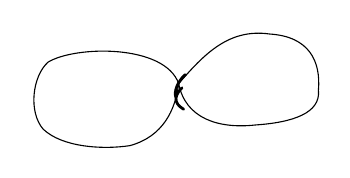
\begin{tikzpicture}[x=1.05cm,y=1.05cm,line cap=round]
\draw (-.02,.12).. controls (-.19,.60) and (-1.27,.58) .. (-1.60,.38)
.. controls (-1.79,.21) and (-1.84,-.22) .. (-1.66,-.43)
.. controls (-1.43,-.65) and (-.94,-.68) .. (-.61,-.63)
.. controls (-.21,-.52) and (-.06,-.20) .. (-.02,.12);
\draw (-.02,.12).. controls (.29,.48) and (.59,.79) .. (1.08,.72)
.. controls (1.56,.69) and (1.70,.39) .. (1.67,.04)
.. controls (1.70,-.24) and (1.35,-.35) .. (.91,-.38)
.. controls (.46,-.43) and (.06,-.30) .. (-.02,.12);
\draw[line width=1pt] (-.05,-.06).. controls (-.09,.03) and (-.02,.16) .. (.06,.23)
(.04,-.19).. controls (-.10,-.11) and (-.06,-.01) .. (.02,.07);
\end{tikzpicture}}\endgroup}
\end{GelfandAdjacentEvidence}
\begin{GelfandAdjacentEvidence}{GELFAND-P000917}{6}


These cohomologies are \uwave{not homotopy invariant}.

\uline{Ordinary homology:}
\begin{equation*}
 \left\{\begin{array}{ll}
 0 & \mathbb{Z}\\
 1 & 0\\
 2 & \mathbb{Z}\dotplus\mathbb{Z}
 \end{array}\right.
\end{equation*}
\Unclear{GELFAND-P000917}{ordinary-homology-cancellation}{A short entry at right of the first row is crossed out. Its beginning resembles $\mathbb Z$, but the entire entry is illegible.}
\end{GelfandAdjacentEvidence}
\begin{GelfandAdjacentEvidence}{GELFAND-P000917}{7}


They do not satisfy Poincaré duality (immediately apparent).

\uline{MacPherson hom.}
\begin{equation*}
 \left\{\begin{array}{ll}
 0 & \mathbb{Z}\dotplus\mathbb{Z}\\
 1 & 0\\
 2 & \mathbb{Z}\dotplus\mathbb{Z}.
 \end{array}\right.
\end{equation*}
\SourceFigure{GELFAND-P000917}{homology-sum-signs}{In all three sums a dot is written above the plus sign.}
\end{GelfandAdjacentEvidence}
\begin{GelfandAdjacentEvidence}{GELFAND-P000917}{8}


\SourceFigure{GELFAND-P000917}{forbidden-simplex}{A bent line joins two marked points and passes through the contact of the outlines.%
\par\smallskip
\begingroup\color{black}\GelfandFitDiagram{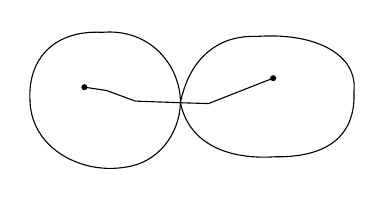
\begin{tikzpicture}[x=1.08cm,y=1.04cm,line cap=round]
\draw (1.80,0) .. controls (1.80,.45) and (1.45,.91) .. (.88,.86)
 .. controls (.31,.89) and (.01,.53) .. (.03,.05)
 .. controls (.03,-.54) and (.61,-.87) .. (1.13,-.79)
 .. controls (1.55,-.74) and (1.79,-.37) .. (1.80,0);
\draw (1.80,0) .. controls (1.89,.47) and (2.18,.83) .. (2.70,.81)
 .. controls (3.39,.86) and (3.89,.59) .. (3.84,.13)
 .. controls (3.86,-.36) and (3.58,-.67) .. (2.91,-.66)
 .. controls (2.30,-.70) and (1.89,-.46) .. (1.80,0);
\draw (.67,.19)--(.93,.15)--(1.27,.02)--(1.80,0)--(2.13,-.01)--(2.89,.30);
\fill (.67,.19) circle (1.1pt) (2.89,.30) circle (1.1pt);
\end{tikzpicture}}\endgroup}
\end{GelfandAdjacentEvidence}
\begin{GelfandAdjacentEvidence}{GELFAND-P000917}{9}

Such a simplex \uwave{is forbidden}.

\uline{Conjecture:} they agree with $L_2$-cohomology.

(this \uline{interested Borel})

Suppose there is exactly one isol. singularity. Then MF-cohom.
\SourceFigure{GELFAND-P000917}{macpherson-gloss}{‘(MacPhers.)’ is written under ‘MF-cohom.’.}
\end{GelfandAdjacentEvidence}
\begin{GelfandAdjacentEvidence}{GELFAND-P000917}{10}


\begin{equation*}
 \left.\begin{aligned}
 \text{in dim.}\ >\frac{\dim X}{2}\quad &\text{agree with ordinary ones,}\\
 \text{in dim.}\ <\frac{\dim X}{2}\quad &\text{from Poincaré duality.}
 \end{aligned}\right]\quad\text{this is Deligne's def.}
\end{equation*}
\SourceFigure{GELFAND-P000917}{deligne-bracket}{‘This is Deligne’s def.’ is written to the right of the bracket.}
\end{GelfandAdjacentEvidence}



\Needspace{7\baselineskip}
\begin{GelfandAdjacentEvidence}{GELFAND-P000918}{1}
\SourcePage{GELFAND-P000918}{unlabelled}

Deligne's def. in a more general situation (inductive)

\uline{M. I. Graev.}

From the works of Gelf.-Gind.-Shap.
\begin{equation*}
\begin{array}{ll}
 \text{FA} & 13:2\\
 \text{FA} & 14:4
\end{array}
\end{equation*}
\Unclear{GELFAND-P000918}{reference-author-abbreviation}{The last surname is abbreviated ‘Shap.’. The right-hand entries read ‘FA 13:2’ and ‘FA 14:4’.}
\end{GelfandAdjacentEvidence}
\begin{GelfandAdjacentEvidence}{GELFAND-P000918}{2}


$\mathcal D\subset\mathbb R^n$,

$(n+k-1)$-param. family of curves
\Unclear{GELFAND-P000918}{family-parameter-cancellation}{$(n+k-1)$ is inserted above and linked to the crossed-out entry. The earlier mark is illegible.}
\end{GelfandAdjacentEvidence}
\begin{GelfandAdjacentEvidence}{GELFAND-P000918}{3}


\begin{equation*}
 x_i=\varphi_i(x_1,\xi),\qquad
 \xi=(\xi_1,\ldots,\xi_n),\qquad \xi\in\Gamma
\end{equation*}

Integr. transform
\begin{equation*}
 \xi=(\xi_1,\ldots,\xi_{n+k-1}),
\end{equation*}
\Unclear{GELFAND-P000918}{parameter-vector-length}{The first list ends at $\xi_n$, the second at $\xi_{n+k-1}$.}
\end{GelfandAdjacentEvidence}
\begin{GelfandAdjacentEvidence}{GELFAND-P000918}{4}

$f(x),\qquad \operatorname{supp}f\subset\mathcal D$
\begin{equation*}
 F(\xi)=I_\chi f
 =\int f(x_1,\varphi_1(x_1,\xi),\ldots,\varphi_n(x_1,\xi))
         \chi(x_1,\xi)\,dx_1
\end{equation*}
\Unclear{GELFAND-P000918}{integral-first-index}{The first index on $\varphi$ under the integral reads 1.}
\end{GelfandAdjacentEvidence}
\begin{GelfandAdjacentEvidence}{GELFAND-P000918}{5}

\SourceFigure{GELFAND-P000918}{positive-weight-callout}{An arrow from the annotation to the factor $\chi$.%
\par\smallskip
\begingroup\color{black}\GelfandFitDiagram{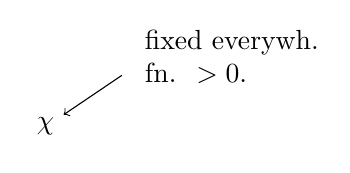
\begin{tikzpicture}
\node[anchor=west,align=left,inner sep=1pt] (W) at (1.22,.88) {fixed everywh.\\fn. \({}>0\).};
\node at (0,0) {$\chi$};
\draw[->] (.97,.65)--(.23,.15);
\end{tikzpicture}}\endgroup}
\end{GelfandAdjacentEvidence}
\begin{GelfandAdjacentEvidence}{GELFAND-P000918}{6}


It is of interest to find such sets of curves for which

\(\exists\) a loc. inversion formula exists (recovery from integrals over curves passing through this point or an infinitesimally close one)

Such sets of curves are called \uwave{admissible}.

$\forall x^0\in\mathcal D$ define an operator \(F(\xi)\longrightarrow\mathcal H_{x^0}F\).
\Unclear{GELFAND-P000918}{differential-operator-glyph}{The operator's script letter is rendered $\mathcal H$.}
\end{GelfandAdjacentEvidence}
\begin{GelfandAdjacentEvidence}{GELFAND-P000918}{7}


\begin{equation*}
 \Gamma_{x^0}\qquad x_i^0=\varphi_i(x_i^0,\xi)
 \qquad\dim\Gamma_{x^0}=k
\end{equation*}
\Unclear{GELFAND-P000918}{fixed-point-coordinate-index}{The dot on the subscript $i$ is visible in the first argument of $\varphi_i$.}
\end{GelfandAdjacentEvidence}
\begin{GelfandAdjacentEvidence}{GELFAND-P000918}{8}

\Unclear{GELFAND-P000918}{gamma-subscript-cancellation}{An illegible mark below $x$ in the subscript of the left-hand $\Gamma$ is crossed out.}
\end{GelfandAdjacentEvidence}
\begin{GelfandAdjacentEvidence}{GELFAND-P000918}{9}


\(\mathcal H_{x^0}\) --- a diff. form on
\Incomplete{GELFAND-P000918}{trailing-form-on}{The line ends with ‘on’. No object is written after it.}
\end{GelfandAdjacentEvidence}
\begin{GelfandAdjacentEvidence}{GELFAND-P000918}{10}


\begin{equation*}
 \mathcal H_{x^0}F=
 \sum a_{ij}(x_1^0,\xi)\frac{\partial F}{\partial\xi_j}\,d\xi_i
 + F\sum b_i(x_1^0,\xi)\,d\xi_i
\end{equation*}

The operator $\mathcal H_{x^0}$ is called \uline{admissible}, if $\forall$ fn. $f$ the diff. form

\(\mathcal H_{x^0}I_\chi f\) is closed.

\(k>1\ \Rightarrow\) this is the complete def.

If $k=1$, it is automatically closed and it is req. that the functional
\begin{equation*}
 f\mapsto\int\mathcal H_{x_0}I_\chi f
\end{equation*}
be concentrated at the point \(x_0\).
\Unclear{GELFAND-P000918}{base-point-zero-position}{In the integral and the next line 0 is a subscript. In the preceding formulas the 0 on $x$ is a superscript.}
\end{GelfandAdjacentEvidence}
\begin{GelfandAdjacentEvidence}{GELFAND-P000918}{11}


Trivial functional: \(\underline{\mathcal H_{x^0}F=d(\mu F)}\)
\SourceFigure{GELFAND-P000918}{trivial-functional-underline}{The formula for the trivial functional is underlined.}
\end{GelfandAdjacentEvidence}


The quotient by the triv. functionals is important.


\clearpage
\pdfbookmark[0]{Chapter 18}{gelfand-archive-chapter-18}
\section*{Chapter 18}
\Needspace{7\baselineskip}
\begin{GelfandAdjacentEvidence}{GELFAND-P000919}{1}
\SourcePage{GELFAND-P000919}{unlabelled}

\uuline{13.10.80}\qquad \uline{Gelfand Sem.}

\uline{I. M. Gelfand.} Consider the equation
\begin{equation*}
 f(z_1,\ldots,z_n;w_1,\ldots,w_n)=0
 \tag{1}
\end{equation*}

Example: consider a 2nd-order diff. eq.
\begin{equation*}
 y''=f(x,y,y')
 \tag{2}
\end{equation*}
\Unclear{GELFAND-P000919}{formula-02-cancelled-superscript}{A superscript mark above the second argument $y$ is crossed out. Its reading is unresolved.}
\end{GelfandAdjacentEvidence}
\begin{GelfandAdjacentEvidence}{GELFAND-P000919}{2}


Then
\begin{equation*}
 y=\varphi(x,\xi,\eta)
 \tag{3}
\end{equation*}
\Unclear{GELFAND-P000919}{formula-03-overwritten-function}{The heavily traced letter reads $\varphi$.}
\end{GelfandAdjacentEvidence}
\begin{GelfandAdjacentEvidence}{GELFAND-P000919}{3}


Conversely, if we have family (3), a 2nd-order diff. eq. is constructed from it.

more generally:
\begin{equation*}
 F(x,y,\xi,\eta)=0
 \tag{4}
\end{equation*}
\Unclear{GELFAND-P000919}{formula-04-separator}{In (4) there is a comma after $y$.}
\end{GelfandAdjacentEvidence}
\begin{GelfandAdjacentEvidence}{GELFAND-P000919}{4}


One can regard $\xi,\eta$ as a point and construct the dual diff. eq.

(1) defines an $n$-param. family of hypersurfaces.

(5) \uwave{Problem:} find the geometry assoc. with this family.

We can make changes of variables. E.g., in the eq. of straight lines
\begin{equation*}
 \xi x+\eta y=1
 \tag{6}
\end{equation*}

(7) \uwave{Problem:} how can we tell whether family (4) reduces to the family of straight lines (6).

\uline{Substitutions:}
\begin{equation*}
 \left\{\begin{aligned}
 x_1&=u(x,y)\\
 y_1&=v(x,y
 \end{aligned}\right.
 \qquad
 \left\{\begin{aligned}
 \xi_1&=\varphi(\xi,\eta)\\
 \eta_1&=\psi(\xi,\eta)
 \end{aligned}\right.
\end{equation*}
\Unclear{GELFAND-P000919}{substitution-missing-parenthesis}{The second line of the left-hand system has no closing parenthesis after $y$.}
\end{GelfandAdjacentEvidence}
\begin{GelfandAdjacentEvidence}{GELFAND-P000919}{5}


(8) \uwave{General definition:} \uline{double fibration}

(9) an element --- \uwave{a point and a curve passing through it}

(curves from a 2-param. family)

\SourceFigure{GELFAND-P000919}{double-fibration}{Two projections labelled $\pi_1$ and $\pi_2$.%
\par\smallskip
\begingroup\color{black}\GelfandFitDiagram{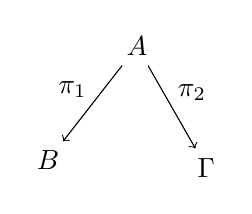
\begin{tikzpicture}
\node (A) at (0,0) {$A$};
\node (B) at (-1.13,-1.45) {$B$};
\node (G) at (.88,-1.54) {$\Gamma$};
\draw[->] (A)--node[above left,inner sep=2pt] {$\pi_1$}(B);
\draw[->] (A)--node[above right,inner sep=2pt] {$\pi_2$}(G);
\end{tikzpicture}}\endgroup
\par
(there are 2 projections)}
\end{GelfandAdjacentEvidence}


(see the article by \uwave{Gelfand}, \uwave{Gindikin}, \uwave{Shapiro} in FA)


\Needspace{7\baselineskip}
\begin{GelfandAdjacentEvidence}{GELFAND-P000920}{1}
\SourcePage{GELFAND-P000920}{unlabelled}

(10) \uwave{Requirement:} if
\begin{equation*}
 \left\{\begin{aligned}
 \pi_1x&=\pi_1x'\\
 \text{and}\quad\pi_2x&=\pi_2x'
 \end{aligned}\right.
 ,\quad\text{then }x=x'
\end{equation*}

a stronger requirement:
\begin{equation*}
 (11)\qquad A\subset B\times\Gamma\quad\text{as a \uwave{submanifold}}
\end{equation*}
\begin{equation*}
 x\mapsto(\pi_1x,\pi_2x)
\end{equation*}

\uline{Problem:} classify up to diffeomorphism
\begin{equation*}
 f(z,w)=0,
 \tag{12}
\end{equation*}
up to changes
\begin{equation*}
 \varphi(z)=z_1,\qquad\psi(w)=w_1
\end{equation*}
(everything analytic).

(13) Another example: $A=G$ --- a group, $K,H$ --- 2 subgroups,
\begin{equation*}
 B=H\backslash G,\qquad\Gamma=K\backslash G.
\end{equation*}

(14) \uline{Important example:}

$G$ --- the group $GL(n,\mathbb C)$,

$K$ --- subgr. of unitary matrices

$H$ --- —\raisebox{-.15ex}{\(\scriptstyle\prime\prime\)}— of triang. matrices

(15) Useful special case: $n=2$.

Then Lobach. geom. and horospheres arise.
\Unclear{GELFAND-P000920}{lobachevsky-abbreviation}{The abbreviation before ‘Lobach.’ reads «пл.», possibly ‘plane’.}
\end{GelfandAdjacentEvidence}
\begin{GelfandAdjacentEvidence}{GELFAND-P000920}{2}


(perhaps take 1 on the main diagonal in $H$)
\Unclear{GELFAND-P000920}{subgroup-parenthesis-word}{The parentheses begin ‘perhaps’.}
\end{GelfandAdjacentEvidence}
\begin{GelfandAdjacentEvidence}{GELFAND-P000920}{3}


Work in Inventiones on \uwave{Segre families.}
\begin{equation*}
 \tau(z,\zeta)=0
 \tag{16}
\end{equation*}

\Unclear{GELFAND-P000920}{right-margin-strokes}{Separate illegible strokes in the right margin level with (16).}
\end{GelfandAdjacentEvidence}
\begin{GelfandAdjacentEvidence}{GELFAND-P000920}{4}


\begin{align*}
 z&=(z_1,\quad,z_n;w)\\
 \zeta&=(\zeta_1,\quad,\zeta_{n+1})
\end{align*}
\Unclear{GELFAND-P000920}{formula-16-tuple-gaps}{In both tuples, the spaces between the commas contain no visible ellipsis.}
\end{GelfandAdjacentEvidence}
\begin{GelfandAdjacentEvidence}{GELFAND-P000920}{5}


\begin{align*}
 \theta&=d_z\tau=\tau_\alpha\,dz^\alpha+\tau_w\,dw\\
 \theta^\alpha&=dz^\alpha\\
 \theta_\alpha&=d\zeta_\alpha
\end{align*}

Under the map
\begin{equation*}
 (z,\zeta)\to(f(z),\bar f(\zeta))
 \tag{17}
\end{equation*}
the forms transform as follows:

\begin{equation*}
 \begin{aligned}
 \theta^*&=\theta,\\
 \theta^{\alpha*}&=\left(\frac{\partial f^\alpha}{\partial z^\beta}
       -\frac{\tau_\beta}{\tau_w}\frac{\partial f^\alpha}{\partial w}\right)\theta^\beta
       +\frac{1}{\tau_w}\frac{\partial f^\alpha}{\partial w}\theta,
 \end{aligned}
 \tag{18}
\end{equation*}
\Incomplete{GELFAND-P000920}{formula-18-upper-cancellation}{An illegible expression is crossed out after the minus sign and before the fraction with $\tau_\beta$.}
\end{GelfandAdjacentEvidence}
\begin{GelfandAdjacentEvidence}{GELFAND-P000920}{6}

\Unclear{GELFAND-P000920}{formula-18-upper-last-denominator}{In the last term the glyph before the subscript $w$ resembles $\tau$ with an angular top. The reading $\tau_w$ is tentative.}
\end{GelfandAdjacentEvidence}
\begin{GelfandAdjacentEvidence}{GELFAND-P000920}{7}


\begin{equation*}
 \begin{aligned}
 \theta_\alpha^*&=\left(\frac{\partial\bar f}{\partial\zeta_\beta}
     -\frac{\tau^\beta}{\tau^\eta}\frac{\partial f^\alpha}{\partial\eta}
     \right)\theta_\beta+\frac{1}{\tau^\beta}\frac{\partial\bar f_\alpha}{\partial\eta}.
 \end{aligned}
\end{equation*}
\Unclear{GELFAND-P000920}{formula-18-first-numerator}{The first numerator of the lower line has a bar above $f$. No index is visible on $f$.}
\end{GelfandAdjacentEvidence}
\begin{GelfandAdjacentEvidence}{GELFAND-P000920}{8}

\Unclear{GELFAND-P000920}{formula-18-overwritten-denominator}{The denominator after the minus sign tentatively has upper index $\eta$. The lower mark is heavily crossed out or overwritten.}
\end{GelfandAdjacentEvidence}
\begin{GelfandAdjacentEvidence}{GELFAND-P000920}{9}

\Unclear{GELFAND-P000920}{formula-18-lower-cancellation}{A long looped cancellation lies between the fraction with $\tau^\beta$ and the next derivative.}
\end{GelfandAdjacentEvidence}
\begin{GelfandAdjacentEvidence}{GELFAND-P000920}{10}

\Unclear{GELFAND-P000920}{formula-18-middle-numerator}{The middle numerator of the lower line has superscript $\alpha$. No bar over $f$ is visible.}
\end{GelfandAdjacentEvidence}
\begin{GelfandAdjacentEvidence}{GELFAND-P000920}{11}

\Unclear{GELFAND-P000920}{formula-18-final-term}{The last denominator reads $\tau^\beta$, and the $\alpha$ on the last $\bar f$ is a subscript. No factor is visible after the derivative.}
\end{GelfandAdjacentEvidence}
\begin{GelfandAdjacentEvidence}{GELFAND-P000920}{12}


[Crossed out: From this.] Let
\SourceFigure{GELFAND-P000920}{cancelled-from-here}{The crossed-out word reads ‘From this’.}
\end{GelfandAdjacentEvidence}


\begin{equation*}
 \tau\mapsto s(z,\zeta)\tau(z,\zeta)
 \tag{19}
\end{equation*}
Then


\Needspace{7\baselineskip}
\begin{GelfandAdjacentEvidence}{GELFAND-P000921}{1}
\SourcePage{GELFAND-P000921}{3}

\begin{equation*}
 \left\{\begin{aligned}
 \theta^*&=s\theta\\
 \theta^{\alpha*}&=\theta^\alpha\\
 \theta_\alpha^*&=\theta_\alpha
 \end{aligned}\right.
 \tag{20}
\end{equation*}

and

\begin{equation*}
 \left\{\begin{aligned}
 \theta^*&=u\theta^*\\
 \theta^\alpha&=u^\alpha\theta^\alpha+u^\alpha_\beta\theta^{\beta*}\\
 \theta_\alpha&=v_\alpha\theta^*+v^\beta_\alpha\theta_\beta^*
 \end{aligned}\right.
 \tag{21}
\end{equation*}
\Unclear{GELFAND-P000921}{formula-21-first-left}{On the left of the first row a heavily traced superscript over $\theta$ is tentatively read as a star.}
\end{GelfandAdjacentEvidence}
\begin{GelfandAdjacentEvidence}{GELFAND-P000921}{2}

\Unclear{GELFAND-P000921}{formula-21-first-right-index}{In the second line the first term on the right reads $u^\alpha\theta^\alpha$, with no visible star.}
\end{GelfandAdjacentEvidence}
\begin{GelfandAdjacentEvidence}{GELFAND-P000921}{3}


(22) A $G$-structure arises, where $G$ is the group
\begin{equation*}
 \begin{pmatrix}
 u&0&0\\
 u^\alpha&u_\beta^\alpha&0\\
 v_\alpha&0&v_\alpha^\beta
 \end{pmatrix}
\end{equation*}

(23) \uwave{Abstr. Segre family:}
[crossed out above: collection?]
[inserted above: (a set with a $G$-struct. and)]
if there is a collection of forms.
\Unclear{GELFAND-P000921}{segre-cancelled-word}{The word crossed out above the line is tentatively ‘collection’.}
\end{GelfandAdjacentEvidence}
\begin{GelfandAdjacentEvidence}{GELFAND-P000921}{4}

\SourceFigure{GELFAND-P000921}{segre-insertion-ending}{A long insertion mark leads to ‘if’. The word after ‘struct.’ reads ‘and’.%
\par\smallskip
\begingroup\color{black}\GelfandFitDiagram{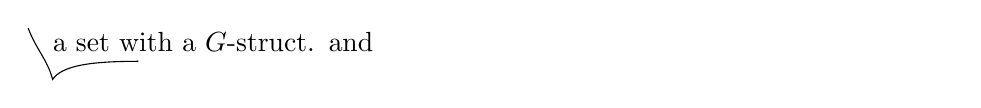
\begin{tikzpicture}
\node[anchor=west,text width=.94\linewidth,align=left,inner sep=1pt] at (.27,.33) {a set with a $G$-struct. and};
\draw (0,.50).. controls (.10,.23) and (.24,.11) .. (.31,-.15)
.. controls (.43,.03) and (.81,.08) .. (1.40,.08);
\end{tikzpicture}}\endgroup}
\end{GelfandAdjacentEvidence}
\begin{GelfandAdjacentEvidence}{GELFAND-P000921}{5}


and the conditions hold
\begin{equation*}
 \left\{\begin{aligned}
 d\theta&\equiv d\theta^\alpha\equiv0\quad(\operatorname{mod}\ \theta,\theta^1,\ldots,\theta^n)\\
 d\theta&\equiv d\theta_\alpha\equiv0\quad(\operatorname{mod}\ \theta,\theta_1,\ldots,\theta_n)
 \end{aligned}\right.
 \tag{24}
\end{equation*}
\SourceFigure{GELFAND-P000921}{formula-24-relation}{Each of the four congruence signs in (24) has three strokes.}
\end{GelfandAdjacentEvidence}


\uuline{Special case of the problem:} what are the invariants of a family of curves in the plane, a family of surf. in 3-dimensional space, etc.


\Needspace{7\baselineskip}
\begin{GelfandAdjacentEvidence}{GELFAND-P000922}{1}
\SourcePage{GELFAND-P000922}{6}

\uuline{20.10.80}\qquad\underline{Gelfand Sem.}

\uuline{A. Goncharov.}\qquad\underline{$G$-structures.}

$M$ --- smooth manifold
\SourceFigure{GELFAND-P000922}{frame-bundle}{Bundle of tangent frames (principal $GL(n,R)$-bundle).%
\par\smallskip
\(\begin{matrix}E\\[-2pt]\downarrow\\[-2pt]M\end{matrix}\)}
\end{GelfandAdjacentEvidence}
\begin{GelfandAdjacentEvidence}{GELFAND-P000922}{2}


\[G\subset GL(n,R)\]

\SourceFigure{GELFAND-P000922}{g-structure}{$G$-structure.%
\par\smallskip
\begingroup\color{black}\GelfandFitDiagram{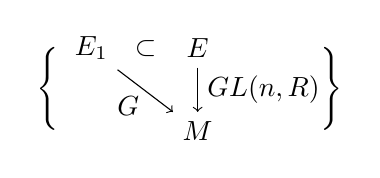
\begin{tikzpicture}[baseline=(E.base),x=1cm,y=1cm]
 \node (Eone) at (0,0) {$E_1$};
 \node at (.69,0) {$\subset$};
 \node (E) at (1.35,0) {$E$};
 \node (M) at (1.35,-1.05) {$M$};
 \draw[->] (Eone.south east) -- node[below left,inner sep=2pt] {$G$} (M.north west);
 \draw[->] (E) -- node[right] {$GL(n,R)$} (M);
 \node at (-.55,-.52) {$\Biggl\{$};
 \node at (3.05,-.52) {$\Biggr\}$};
\end{tikzpicture}}\endgroup}
\end{GelfandAdjacentEvidence}
\begin{GelfandAdjacentEvidence}{GELFAND-P000922}{3}


\underline{Problem:} [crossed out] consider all geometries on $S^2$ associated with the different subgroups $G\subset GL(n,R)$.
\Unclear{GELFAND-P000922}{cancelled-task-word}{The word before ‘consider’ is crossed out and illegible.}
\end{GelfandAdjacentEvidence}
\begin{GelfandAdjacentEvidence}{GELFAND-P000922}{4}


\uuline{D. B. Fuchs.}\quad\underline{On cohomologies according to Deligne, MacPherson, etc.}

\hspace{2em}\uuline{according to MacPherson.}

$X$ --- set with sing., i.e. there is a stratification
\begin{equation*}
 X=X_n\supset X_{n-1}\supset\ldots\supset X_0.
 \tag{1}
\end{equation*}

$X_i-X_{i-1}$ --- smooth $2i$-dimensional set

and a certain natural condition of local triviality

\SourceFigure{GELFAND-P000922}{stratum}{Sketch accompanying the local triviality condition.%
\par\smallskip
\begingroup\color{black}\GelfandFitDiagram{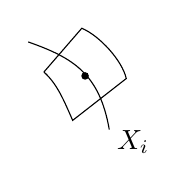
\begin{tikzpicture}[scale=.83]
 \draw (.31,1.01) -- (.89,1.68)
    .. controls (1.17,1.56) and (1.51,1.18) .. (1.57,.91)
    -- (.75,.27) .. controls (.61,.59) and (.51,.83) .. (.31,1.01);
 \draw (.07,1.47) .. controls (.75,1.23) and (1.16,.99) .. (1.31,.13);
 \fill (.94,.95) circle (.058);
 \node[anchor=north west,inner sep=0pt] at (1.42,.12) {$X_i$};
\end{tikzpicture}}\endgroup}
\end{GelfandAdjacentEvidence}
\begin{GelfandAdjacentEvidence}{GELFAND-P000922}{5}


A point $x_0\in X_i$ has a neighb. $U$ such that

in the stratification
\begin{equation*}
 U\supset U\cap X_{n-1}\supset U\cap X_{n-1}\supset\ldots\supset U\cap X_i
 \tag{2}
\end{equation*}
[crossed out: ‘diffeomorphic’ (?) […] ‘stratification’ (?)]

has the same structure at every point of $U\cap X_i$
\SourceFigure{GELFAND-P000922}{stratification-repeated-index}{The term $U\cap X_{n-1}$ is written twice in succession in (2).}
\end{GelfandAdjacentEvidence}
\begin{GelfandAdjacentEvidence}{GELFAND-P000922}{6}

\Incomplete{GELFAND-P000922}{cancelled-local-triviality}{The middle of the crossed-out line is illegible. The beginning and ending are tentative readings.}
\end{GelfandAdjacentEvidence}
\begin{GelfandAdjacentEvidence}{GELFAND-P000922}{7}


Consider cycles of [circled and inserted above: sing.] simplices $\sigma^q$ for which
\begin{equation*}
 \dim(\sigma^q\cap X_{n-i})\leq q-i
 \qquad (\operatorname{Codim}X_{n-i}=2i\,!)
 \tag{3}
\end{equation*}

(like the condition that would hold in general pos. with respect to the distinguished part)

If the right side is $q$ or $q-2i$ (!), one gets ordinary cohomology.

Quotient by [crossed out above] the boundaries of chains subject to an analogous condition.
\Unclear{GELFAND-P000922}{correction-above-boundaries}{The crossed-out sign before ‘boundaries’ is illegible.}
\end{GelfandAdjacentEvidence}


\uwave{Another defn., hypothetically equiv. to this one}

Deligne wanted it to work over finite fields.

a more spec. reason: there is hope of proving a connection with $L^2$-cohomology

($L^2$ [inserted below: -forms] on approaching the stratum)

\underline{A. Beilinson.}\quad The defn. above can be given a local form (pass to a complex of sheaves, its cohom. will be MacPherson cohom.).


\Needspace{7\baselineskip}
\begin{GelfandAdjacentEvidence}{GELFAND-P000923}{1}
\SourcePage{GELFAND-P000923}{unlabelled}

Now the same using diff. operators

Embed
\[
 X\hookrightarrow\underset{\text{set [without singularities]}}{Y}
\]
\begin{equation*}
 X_{\mathrm{reg}}=X_n-X_{n-1}\hookrightarrow X\hookrightarrow Y.
 \tag{4}
\end{equation*}

On $X_n-X_{n-1}$ consider the triv. system of diff. eqs., i.e.

the sheaf $\mathcal O_{X_{\mathrm{reg}}}$, the sheaf of fns., also a sheaf of modules over the ring of diff. op.

We want to extend this to all of $Y$.

\underline{Example:}

$X$ --- a cross, \qquad $Y$ --- the plane
\SourceFigure{GELFAND-P000923}{example-cross-left-point}{Four arrows point inward. There is a separate dot to the left of the left arrow. Its role in the diagram is uncertain.%
\par\smallskip
\begingroup\color{black}\GelfandFitDiagram{\begin{tikzpicture}[scale=.8]
 \draw[->] (-1.53,.03) .. controls (-1.0,.10) and (-.62,.07) .. (-.14,.02);
 \draw[->] (1.09,-.02) -- (.13,-.02);
 \draw[->] (.08,1.02) -- (.01,.13);
 \draw[->] (-.18,-.97) -- (-.07,-.12);
 \fill (-1.67,.02) circle (.026);
\end{tikzpicture}}\endgroup}
\end{GelfandAdjacentEvidence}
\begin{GelfandAdjacentEvidence}{GELFAND-P000923}{2}


extend the fns. by tensoring with $\delta$ in the transverse direction

Diff. operators act on them.

(and the same in the general case)

Along $X$ they must be reg. (and supported on $X$).

Consider the sheaf
\begin{equation*}
 U\longrightarrow\text{all sections over}\;(Y-X_{\mathrm{sing}})\;\text{of the constructed sheaf}.
\end{equation*}
\SourceFigure{GELFAND-P000923}{sheaf-sections-domain}{After ‘over’, the manuscript gives $(Y-X_{\mathrm{sing}})$ without an intersection with $U$.}
\end{GelfandAdjacentEvidence}
\begin{GelfandAdjacentEvidence}{GELFAND-P000923}{3}


(5)\quad (direct image in the sense of sheaf theory under the embedding $\underline{Y-X_{\mathrm{sing}}\overset{i}{\hookrightarrow}Y}.$)

(6)\quad \underline{Thm. 1.}

This sheaf of modules has a \uwave{unique irred. submodule}!

(\underline{Moral} (I.M.G.) in the theory of sing. one should work with diff. operators.)

Thus a module over the ring of diff. op. over $Y$ is constructed.

(sheaf of modules)

On $X_{\mathrm{reg}}$ consider the sheaf of fns. and extend them by $\delta$-fns. in the transv. dir.

On $Y\setminus X_{\mathrm{sing}}$ obtain a module over diff. op. (with holom. or algebr. coeffs.)
\Unclear{GELFAND-P000923}{overwritten-sing-index}{The subscript on this line is overwritten. The final reading is ‘sing’.}
\end{GelfandAdjacentEvidence}
\begin{GelfandAdjacentEvidence}{GELFAND-P000923}{4}


\uwave{Extend into the singularity} $X_{\mathrm{sing}}$.

The module is constr. in 2 steps

\underline{Step 1.} Maximal --- the direct image of the sheaf.

\underline{Step 2.} Take the irred. submodule (it is unique!!)

\underline{Here:} regular along $X$, but without compatibility!
\SourceFigure{GELFAND-P000923}{cross-four-limits}{(4 different limits!)%
\par\smallskip
\begingroup\color{black}\GelfandFitDiagram{\begin{tikzpicture}[scale=.72]
 \draw (-.84,0) -- (.96,.03);
 \draw (-.15,-.8) .. controls (-.10,-.43) and (.12,.39) .. (.05,.73);
 \fill (0,.014) circle (.064);
\end{tikzpicture}}\endgroup}
\end{GelfandAdjacentEvidence}
\begin{GelfandAdjacentEvidence}{GELFAND-P000923}{5}


[crossed out above] Consider a resolution of this module $M$
\Incomplete{GELFAND-P000923}{cancelled-resolution-word}{The word above ‘resolution’ is heavily crossed out and illegible.}
\end{GelfandAdjacentEvidence}
\begin{GelfandAdjacentEvidence}{GELFAND-P000923}{6}

\begin{equation*}
 \ldots\longrightarrow F_1\longrightarrow F_0\longrightarrow M\longrightarrow0
 \tag{7}
\end{equation*}

($F_j$ --- free module over diff. op. [crossed out] $\mathcal D_Y$)
\Unclear{GELFAND-P000923}{cancelled-ring-symbol}{The cancelled sign before $\mathcal D_Y$ is illegible.}
\end{GelfandAdjacentEvidence}


and map into fns. over $Y$ (into $\mathcal O_Y$)


\Needspace{7\baselineskip}
\begin{GelfandAdjacentEvidence}{GELFAND-P000924}{1}
\SourcePage{GELFAND-P000924}{7}

\[\bullet\longrightarrow F_1\longrightarrow F_0\longrightarrow M\longrightarrow0\]

A complex arises:
\begin{equation*}
 \operatorname{Hom}_{\mathcal D}(F_0,\mathcal O_Y)
 \longrightarrow \operatorname{Hom}_{\mathcal D}(F_1,\mathcal O_Y)
 \longrightarrow\ldots
 \tag{8}
\end{equation*}
\SourceFigure{GELFAND-P000924}{complex-verb-letter}{The abbreviation before ‘complex’ reads «Возн.», ‘arises’.}
\end{GelfandAdjacentEvidence}
\begin{GelfandAdjacentEvidence}{GELFAND-P000924}{2}


up to $\operatorname{Codim}_Y X$ this is \uwave{acyclic}, then MacPherson cohomology

(9)\quad \uwave{The simplest overd. syst. of diff. eqs.} --- those for which there is locally a max. number of

(10)\quad solutions (reduce to the system $\dfrac{\partial u}{\partial x_1}=0,\ldots,\dfrac{\partial u}{\partial x_n}=0$) --- they are wholly (?) determ. by the syst.

of their solns. --- there will be a locally constant sheaf on the set.
\Unclear{GELFAND-P000924}{systems-abbreviation}{The abbreviation after ‘they’ is tentatively read as «цел.» (‘wholly’).}
\end{GelfandAdjacentEvidence}
\begin{GelfandAdjacentEvidence}{GELFAND-P000924}{3}


The solns. are locally $\mathrm{const}$.

There may be no global solns.

Analogue in the general sit.

Consider any overd. syst.

(11)\quad If the syst. has \uwave{reg. singularities} (there is a defn.), then the solutions are

--- the MacPherson complex.
\SourceFigure{GELFAND-P000924}{fuchsian-annotation}{Right-hand annotation. The arrow points to ‘reg. singularities’ in (11).%
\par\smallskip
\(\uparrow\)\enspace generaliz. of the notion of a Fuchsian syst.}
\end{GelfandAdjacentEvidence}
\begin{GelfandAdjacentEvidence}{GELFAND-P000924}{4}


This establ. a corresp. between these complexes and syst. with reg. sing.

\underline{Definition} (\underline{Kashiwara}) \uwave{syst. with reg. sing.}

Classical defn. (for syst. of ordinary eqs.) --- reg. sing. (Fuchsian syst.):
\begin{equation*}
 \frac{dx}{dt}=\frac1t A(t)x,\quad\text{where }A\text{ is reg}.
 \tag{12}
\end{equation*}
(first-order syst.)

Let [crossed out] a $\mathcal D$-module $M$ be given (assoc. with an overd. syst.)
\Unclear{GELFAND-P000924}{cancelled-before-module}{The writing crossed out before ‘given’ is illegible.}
\end{GelfandAdjacentEvidence}
\begin{GelfandAdjacentEvidence}{GELFAND-P000924}{5}


(13)\quad a) Let $M$ have no torsion, i.e. if $x\in M$, $x\ne0$,

$f\in\mathcal D$, $f\ne0$, then $fx\ne0$.
\SourceFigure{GELFAND-P000924}{torsion-ring}{The shape of the letter in $f\in\mathcal D$ matches $\mathcal D$ in the line about the module.}
\end{GelfandAdjacentEvidence}
\begin{GelfandAdjacentEvidence}{GELFAND-P000924}{6}

\SourceFigure{GELFAND-P000924}{torsion-margin}{At right: (nothing is supported along sets)}
\end{GelfandAdjacentEvidence}
\begin{GelfandAdjacentEvidence}{GELFAND-P000924}{7}


[crossed out: Then […] req. that the restr. along a suff. reg. curve ha[…] form (12)]
\Incomplete{GELFAND-P000924}{cancelled-restriction-word}{The heavily crossed-out word after ‘Then’ is illegible.}
\end{GelfandAdjacentEvidence}
\begin{GelfandAdjacentEvidence}{GELFAND-P000924}{8}

\Incomplete{GELFAND-P000924}{cancelled-restriction-ending}{Before ‘form (12)’ the beginning «име-» (‘ha-’) is visible.}
\end{GelfandAdjacentEvidence}
\begin{GelfandAdjacentEvidence}{GELFAND-P000924}{9}


(14)\quad Then it reduces to syst. (10)

(15)\quad \underline{Claim.} $M$ has reg. sing. $\Longleftrightarrow$ the restr. along a suff. reg. curve has form (12)
\SourceFigure{GELFAND-P000924}{assertion-restriction}{The abbreviation after the equivalence sign reads «суж.» (‘restr.’), as in the crossed-out line above.}
\end{GelfandAdjacentEvidence}
\begin{GelfandAdjacentEvidence}{GELFAND-P000924}{10}


\underline{General defn.} In $\forall$ module there is a filtration

(finite length!) and the irred. factors has form (10) ---

--- integrable connection.
\SourceFigure{GELFAND-P000924}{filtration-verb}{The line about the factors uses the singular verb ‘has’.}
\end{GelfandAdjacentEvidence}


\underline{Defn.} Each irred. compon. must have reg. sing.


\Needspace{7\baselineskip}
\begin{GelfandAdjacentEvidence}{GELFAND-P000925}{1}
\SourcePage{GELFAND-P000925}{unlabelled}

\underline{27.10.80}\qquad\uuline{Gelfand Sem.}

\dotuline{Problems (for first-year students)}

1.\enspace Find all subgroups and norm. subgroups of the symmetry group (?) of regular polyhedra and of the symmetric group.
\Unclear{GELFAND-P000925}{task1-group-ending}{The ending of the word before ‘symmetry’ is heavily overwritten. The construction suggests the genitive «группы» (‘of the group’). The ending is illegible.}
\end{GelfandAdjacentEvidence}
\begin{GelfandAdjacentEvidence}{GELFAND-P000925}{2}


2.\enspace Is the group $SL(2,R)$ simply connected? Construct its univ. cover.
\begin{gather*}
 \alpha\delta-\beta\gamma=1
 \;\Longleftrightarrow\;
 \alpha_1^2-\alpha_2^2-\alpha_3^2+\alpha_4^2=1\\
 \Longleftrightarrow\;
 \alpha_1^2+\alpha_4^2=1+\alpha_2^2+\alpha_3^2
 \;\Longleftrightarrow\\
 \Longleftrightarrow\;
 \left(\underbrace{\frac{\alpha_1}{\sqrt{1+\alpha_2^2+\alpha_3^2}}}_{x_1}\right)^2+
 \left(\underbrace{\frac{\alpha_4}{\sqrt{1+\alpha_2^2+\alpha_3^2}}}_{x_2}\right)^2=1.
\end{gather*}
\Unclear{GELFAND-P000925}{circle-index-corrections}{The subscripts $3$ in the first denominator, $4$ in the second numerator and $2$ in the second denominator are overwritten. The original signs are illegible.}
\end{GelfandAdjacentEvidence}


\[
 \underset{\text{homotopy equiv.}}{(\alpha_1,\alpha_2,\alpha_3,\alpha_4)}
 \longmapsto (x_1,x_2)\in S^1
\]

More precisely, one obtains
\[
 SL(2,R)\underset{\text{diffeom.}}{\cong} S^1\times R^2.
\]

3.\enspace How is the univ. cover of $SL(2,R)$ structured as a group?


\Needspace{7\baselineskip}
\begin{GelfandAdjacentEvidence}{GELFAND-P000926}{1}
\SourcePage{GELFAND-P000926}{unlabelled}

Suppose there are 3 lines
\SourceFigure{GELFAND-P000926}{three-lines}{Three lines labelled $\ell_1,\ell_2,\ell_3$.%
\par\smallskip
\begingroup\color{black}\GelfandFitDiagram{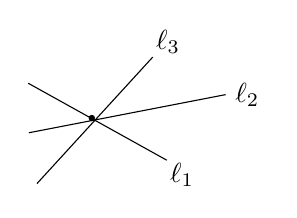
\begin{tikzpicture}[scale=.85]
 \draw (-.95,.52) -- (1.12,-.63) node[below right,inner sep=1pt] {$\ell_1$};
 \draw (-.94,-.22) -- (2.0,.35) node[right] {$\ell_2$};
 \draw (-.82,-.98) -- (.91,.91) node[above right,inner sep=1pt] {$\ell_3$};
 \fill (0,0) circle (.048);
\end{tikzpicture}}\endgroup}
\end{GelfandAdjacentEvidence}
\begin{GelfandAdjacentEvidence}{GELFAND-P000926}{2}

\[
 [?](\ell_1,\ell_2,\ell_3)=
 \begin{cases}
 +1 & \text{if $\ell_2$ is inside $\widehat{\ell_1\ell_3}$ (angle $<\pi$).}\\
 -1 & \text{otherwise}
 \end{cases}
\]
\Unclear{GELFAND-P000926}{triple-sign-name}{The sign before the arguments is heavily overwritten. Possible readings are $\tau$ and $f$. The right-hand note uses $f$ for the three-argument function.}
\end{GelfandAdjacentEvidence}
\begin{GelfandAdjacentEvidence}{GELFAND-P000926}{3}


$(g_j,n_j)$ --- an element, $g_j\in SL(2,C)$
\SourceFigure{GELFAND-P000926}{group-field}{This line reads $C$. Question 3 on the preceding frame has $R$.}
\end{GelfandAdjacentEvidence}
\begin{GelfandAdjacentEvidence}{GELFAND-P000926}{4}


\[
 (g_1,n_1)(g_2,n_2)=(g_1g_2,n_1+n_2+\tau(g_1,g_2))
\]
[crossed out $\tau(\ell_1,g_1\ell_2,g_1g_2\ell_3)$; inserted above the formula $\tau(g_1,g_2)$.]
\Incomplete{GELFAND-P000926}{product-cancellation}{A second, more heavily cancelled entry follows $n_1+n_2+$. Its reading is unresolved.}
\end{GelfandAdjacentEvidence}
\begin{GelfandAdjacentEvidence}{GELFAND-P000926}{5}


$(\ell_1,\ell_2,\ell_3)$ can be chosen arbitrarily, leading to a homolog. cocycle
\begin{gather*}
 g=\begin{pmatrix}\alpha&\beta\\0&\alpha^{-1}\end{pmatrix}
 \qquad
 \varphi(g)=\begin{cases}1,&\alpha>0\\-1,&\alpha<0\end{cases}\\[4pt]
 g=\begin{pmatrix}a&b\\c&d\end{pmatrix}
 \qquad
 \varphi(g)=\begin{cases}i&c>0\\-i&c<0\end{cases}
\end{gather*}
(if it does not reduce to triang.)
\[
 \varphi(g,n)=e^{i\frac{\pi}{2}n}\varphi(g)
\]
\SourceFigure{GELFAND-P000926}{scalar-function-name}{The $\varphi$ in the exponential formula has the same loop as in the two formulas above and in the definition of $\widetilde G$.}
\end{GelfandAdjacentEvidence}
\begin{GelfandAdjacentEvidence}{GELFAND-P000926}{6}


Now take
\[
 \widetilde G=\{(g,n):\varphi(g,n)=1\}
\]
$\widetilde G$ --- this is a group and it is the univ. cover.

\medskip
[at right]
(Here $\ell_3=\ell$ is the $X$-axis)
\[
 \tau(g_1,g_2)=f(\ell,g_1\ell\,g_1g_2\ell)=\pm1
\]
\Unclear{GELFAND-P000926}{triple-argument-divider}{Between the second and third arguments a separate comma cannot be distinguished.}
\end{GelfandAdjacentEvidence}
\begin{GelfandAdjacentEvidence}{GELFAND-P000926}{7}


$\ell$ --- an oriented line

(invar. of a triple of [inserted below and circled: oriented] lines; index of a triple of lines;
\SourceFigure{GELFAND-P000926}{directed-insertion}{The abbreviation for ‘oriented’ is circled and linked to the first occurrence of ‘lines’.}
\end{GelfandAdjacentEvidence}
\begin{GelfandAdjacentEvidence}{GELFAND-P000926}{8}


$+1$ if $g_1\ell$ is between $\ell$ and $g_1g_2\ell$

\uwave{This group is disconnected} --- there are 4 pieces; then take a conn. comp.

4.\enspace (Kirillov). Describe all locally projective structures on $R$

(covered by charts, transition --- fractional-lin. transf.)

atlases are equiv. if the transition is a fract.-lin. transf.

\underline{Answer}: there are countably many loc. project. structures

\uwave{Example 1}. $R$ and param. $t$

\uwave{Example 2}:
\SourceFigure{GELFAND-P000926}{projective-charts}{Two upper axes $t$, $s$ with zeros, and the lower axis $x$.%
\par\smallskip
\begingroup\color{black}\GelfandFitDiagram{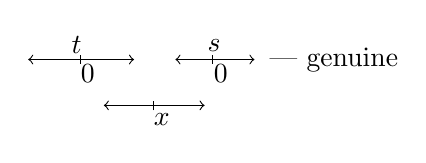
\begin{tikzpicture}[scale=.64]
 \draw[<->] (0,0) -- (2.1,0);
 \draw (1.04,-.08) -- (1.04,.09);
 \node at (.96,.28) {$t$};
 \node at (1.18,-.28) {$0$};
 \draw[<->] (2.92,0) -- (4.49,0);
 \draw (3.65,-.08) -- (3.65,.09);
 \node at (3.69,.28) {$s$};
 \node at (3.82,-.28) {$0$};
 \node[anchor=west,inner sep=0pt] at (4.78,0) {--- genuine};
 \draw[<->] (1.5,-.91) -- (3.5,-.91);
 \draw (2.48,-1.01) -- (2.48,-.82);
 \node at (2.65,-1.2) {$x$};
\end{tikzpicture}}\endgroup}
\end{GelfandAdjacentEvidence}
\begin{GelfandAdjacentEvidence}{GELFAND-P000926}{9}


\dotuline{Relations:} $tx=-1,\quad xs=-1$

When one ends --- go to the other, etc.

The second is not equiv. to the first.

A 2-sheeted cover of the project. line has a loc. project. structure.

A cover of the project. line --- its project. transf. will be --- transf. of the univ. cover.

\uuline{Prof. Gaveau} (\uwave{from Paris})\qquad\underline{3 possible topics.}
\SourceFigure{GELFAND-P000926}{paris-arrow}{Annotation above the line with a leader to ‘from Paris’.%
\par\smallskip
\(\leftarrow\)\enspace\underline{Univ. Paris VI}}
\end{GelfandAdjacentEvidence}
\begin{GelfandAdjacentEvidence}{GELFAND-P000926}{10}


1.\enspace Constr. of envelopes of holomorphy

2.\enspace Constr. of measures on certain $\infty$-dim. homog. sets

3.\enspace Scattering theory and functional integrals.
\SourceFigure{GELFAND-P000926}{gaveau-marginal}{At right: Gaveau is a student of Malliavin, who is now working on stochastic diff. geometry.}
\end{GelfandAdjacentEvidence}
\begin{GelfandAdjacentEvidence}{GELFAND-P000926}{11}


1.\enspace\dotuline{On constructions of envelopes of holomorphy.}

Consider $C^2$ and try to constr. the envelope of holom. of a compact 2-dimensional surf. (in $C^2$)

\uuline{Problem.} Find such a [crossed out] Levi-flat hypersurf. $M$ that
\[
 \partial M=S^2
\]
(the Levi form on it must be $=0$)
\Incomplete{GELFAND-P000926}{levi-cancellation}{The word before ‘Levi-flat’ is heavily crossed out and illegible.}
\end{GelfandAdjacentEvidence}
\begin{GelfandAdjacentEvidence}{GELFAND-P000926}{12}


A Levi-flat region is foliated into compl. leaves

(On the torus this problem cannot be solved)
\SourceFigure{GELFAND-P000926}{levi-foliation}{At the top of the oval is a short dark stroke whose direction is unclear.%
\par\smallskip
\begingroup\color{black}\GelfandFitDiagram{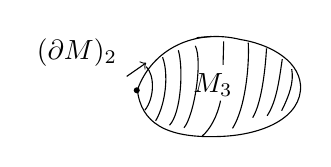
\begin{tikzpicture}[scale=.80]
 \draw (-1.22,-.03)
 .. controls (-.99,.62) and (-.31,.95) .. (.42,.77)
 .. controls (.81,.71) and (1.33,.48) .. (1.37,.05)
 .. controls (1.40,-.47) and (.76,-.76) .. (.03,-.77)
 .. controls (-.77,-.79) and (-1.16,-.55) .. cycle;
 \draw (-1.08,.34) .. controls (-.94,.20) and (-.95,-.16) .. (-1.10,-.35);
 \draw (-.82,.49) .. controls (-.72,.22) and (-.77,-.25) .. (-.93,-.52);
 \draw (-.57,.60) .. controls (-.49,.33) and (-.52,-.39) .. (-.71,-.59);
 \draw (-.30,.67) .. controls (-.18,.42) and (-.32,-.44) .. (-.48,-.63);
 \draw (.15,.74) -- (.14,.37);
 \draw (.10,-.20) .. controls (.05,-.45) and (-.07,-.66) .. (-.19,-.76);
 \draw (.54,.72) .. controls (.56,.39) and (.50,-.31) .. (.29,-.64);
 \draw (.83,.63) .. controls (.81,.28) and (.75,-.24) .. (.61,-.47);
 \draw (1.08,.46) .. controls (1.03,.12) and (.99,-.21) .. (.84,-.44);
 \draw (1.23,.30) .. controls (1.27,.09) and (1.18,-.14) .. (1.07,-.36);
 \draw (-.28,.80) -- (-.04,.82);
 \fill (-1.23,-.035) circle (.048);
 \node at (-.02,.05) {$M_3$};
 \node (boundary) at (-2.18,.56) {$(\partial M)_2$};
 \draw[->] (boundary.south east) -- (-1.08,.40);
\end{tikzpicture}}\endgroup%
\par\dotuline{covering by discs} (foliation)}
\end{GelfandAdjacentEvidence}



\Needspace{7\baselineskip}
\begin{GelfandAdjacentEvidence}{GELFAND-P000927}{1}
\SourcePage{GELFAND-P000927}{11}

There are sing. points of the foliation $\Rightarrow$ the index of the degen. (?) Riemann prob. $=0$ $\Rightarrow$ it is solvable
\Unclear{GELFAND-P000927}{top-index-abbreviation}{The abbreviation before ‘Riemann prob.’ is tentatively «вырожд.» or «вырож.» (‘degen.’).}
\end{GelfandAdjacentEvidence}
\begin{GelfandAdjacentEvidence}{GELFAND-P000927}{2}


(Bishop --- \underline{there arises} \underline{a sing.} integro-diff. eq.)

\underline{2-3}.

$M$ --- a set, $G$ --- a comp. Lie group; $g$ --- a Lie alg.

$\Lambda^1(M,g)$ --- 1-forms on $M$ with vals. in $g$.
\Unclear{GELFAND-P000927}{forms-cancelled-index}{The subscript on $\Lambda$ is crossed out. It may be the digit $2$.}
\end{GelfandAdjacentEvidence}
\begin{GelfandAdjacentEvidence}{GELFAND-P000927}{3}

\SourceFigure{GELFAND-P000927}{yang-mills-margin}{At right: ‘we want to quantize Yang–Mills’.}
\end{GelfandAdjacentEvidence}
\begin{GelfandAdjacentEvidence}{GELFAND-P000927}{4}


\begin{equation*}
 e^{-\int_M\operatorname{Tr}(\Omega\Omega)}D(\omega)
 \tag{1}
\end{equation*}
\SourceFigure{GELFAND-P000927}{curvature-annotations}{Curvature and connection are labelled below (1).%
\par\smallskip
\begingroup\color{black}\GelfandFitDiagram{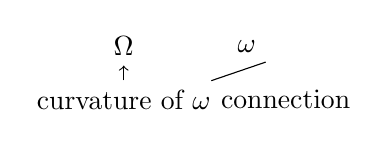
\begin{tikzpicture}[scale=.77]
 \node (Omega) at (0,0) {$\Omega$};
 \node (omega) at (2.03,0) {$\omega$};
 \node (curv) at (0,-.88) {curvature of \(\omega\)};
 \node (conn) at (2.67,-.88) {connection};
 \draw[->] (curv) -- (Omega);
 \draw (omega.south east) -- (conn.north west);
\end{tikzpicture}}\endgroup}
\end{GelfandAdjacentEvidence}
\begin{GelfandAdjacentEvidence}{GELFAND-P000927}{5}


(Formal Feynman integral)

\uwave{Group:} $g\in C(M,G)$ (gauge)
\begin{equation*}
 g\cdot\omega=g^{-1}dg+g^{-1}\omega g
 \tag{2}
\end{equation*}
\Incomplete{GELFAND-P000927}{gauge-cancellation}{The expression crossed out immediately after the second $g^{-1}$ is illegible.}
\end{GelfandAdjacentEvidence}
\begin{GelfandAdjacentEvidence}{GELFAND-P000927}{6}


Goal --- construct a measure inv. under the \dotuline{gauge} [crossed out] \underline{group}.
\Unclear{GELFAND-P000927}{group-word-cancellation}{A short entry before ‘group’ is crossed out. It may read «гр.» (‘grp.’).}
\end{GelfandAdjacentEvidence}
\begin{GelfandAdjacentEvidence}{GELFAND-P000927}{7}


(easier than on the quotient space)

We must integrate over the set of paths in $\Lambda^1$.
\begin{equation*}
 e^{-\int_0^t dt\int_M\operatorname{Tr}(\Omega_t\Omega_t)\,dx}D(\omega_t).
 \tag{3}
\end{equation*}

We will be constructed a family of measures, ‘approx.’ to the equil. measure.
\SourceFigure{GELFAND-P000927}{measure-family-verb}{The manuscript reads «Будем построено», literally ‘we will be constructed’.}
\end{GelfandAdjacentEvidence}
\begin{GelfandAdjacentEvidence}{GELFAND-P000927}{8}

\SourceFigure{GELFAND-P000927}{gauge-orbit-figure}{Orbits, the point $\Pi$ and two lines issuing from it.%
\par\smallskip
\begingroup\color{black}\GelfandFitDiagram{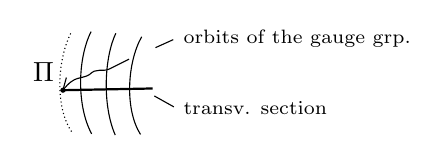
\begin{tikzpicture}[scale=.73]
 \draw[densely dotted] (.25,-.82) .. controls (-.01,-.45) and (-.03,.35) .. (.24,.90);
 \draw (.16,.12) -- (.10,-.10);
 \draw (.60,-.86) .. controls (.34,-.38) and (.35,.44) .. (.59,.92);
 \draw (1.01,-.88) .. controls (.78,-.35) and (.82,.47) .. (1.02,.89);
 \draw (1.45,-.87) .. controls (1.17,-.43) and (1.22,.39) .. (1.47,.83);
 \fill (.10,-.10) circle (.045);
 \node[anchor=east,inner sep=2pt] at (.05,.21) {$\Pi$};
 \draw[thick] (.10,-.10) -- (1.66,-.07);
 \draw (.10,-.10) .. controls (.31,.17) and (.40,.08) .. (.56,.17)
 .. controls (.68,.30) and (.79,.21) .. (.91,.27) -- (1.25,.44);
 \draw (1.71,.64) -- (2.02,.78);
 \node[anchor=west,align=left,inner sep=1pt] at (2.14,.79) {\scriptsize orbits of the gauge grp.};
 \draw (1.69,-.20) -- (2.03,-.39);
 \node[anchor=west,align=left,inner sep=1pt] at (2.14,-.41) {\scriptsize transv. section};
\end{tikzpicture}}\endgroup}
\end{GelfandAdjacentEvidence}
\begin{GelfandAdjacentEvidence}{GELFAND-P000927}{9}


\uwave{At first} --- a kind of Wiener measure on paths.

We need something like an ellipt. operator on the space of connections, inv. under the gauge group.
\[
 \Pi\to d_\Pi\text{ --- covar. diff.},\qquad
 \Box_\Pi=d_\Pi^*d_\Pi+d_\Pi d_\Pi^*
\]
\begin{equation*}
 e^{-\tau\Box_\Pi}(x,y)=p_\tau^{(\Pi)}(x,y)
 \qquad\text{--- \uuline{symbol} of the func.}
 \tag{4}
\end{equation*}
\SourceFigure{GELFAND-P000927}{heat-word}{The word ‘symbol’ is double-underlined after (4).}
\end{GelfandAdjacentEvidence}
\begin{GelfandAdjacentEvidence}{GELFAND-P000927}{10}

\begin{equation*}
 L\varphi(\Pi)=\iint_{M\times M} e^{-\tau\Box_\Pi}(x,y)
 \frac{\delta^2\varphi}{\delta\Pi(x)\delta\Pi(y)}\,dx\,dy
 \tag{5}
\end{equation*}

[crossed out] \uwave{\(\tau\) fixed}.
\Incomplete{GELFAND-P000927}{fixed-tau-cancellation}{A sign or short word before $\tau$ is crossed out. The reading is unresolved.}
\end{GelfandAdjacentEvidence}


One cannot work in Sob. spaces.
\begin{equation*}
 \Lambda^1_{k,\alpha}(M,g),\quad 0<\alpha<1,
 \tag{6}
\end{equation*}
--- some space (Hölder)

The $k$th deriv. is Hölder with exponent $\alpha$.

We need:
\begin{equation*}
 \left\|e^{-\tau\Box_\Pi}-e^{-\tau\Box_{\Pi'}}\right\|_{HS}
 \le C\|\Pi-\Pi'\|
 \tag{7}
\end{equation*}
[under \(HS\): Hilb.–Schmidt.]


\Needspace{7\baselineskip}
\begin{GelfandAdjacentEvidence}{GELFAND-P000928}{1}
\SourcePage{GELFAND-P000928}{unlabelled}

One obtains
\begin{equation*}
 \left\|e^{-\tau\Box_\Pi}-e^{-\tau\Box_{\Pi'}}\right\|_{HS(L^2,L^2)}
 \le C\|\Pi-\Pi'\|_{k,\alpha}
 \tag{8}
\end{equation*}
\SourceFigure{GELFAND-P000928}{eq8-bound}{In (8) there is a slanting stroke beneath $<$. The sign reads $\le$.}
\end{GelfandAdjacentEvidence}
\begin{GelfandAdjacentEvidence}{GELFAND-P000928}{2}


Techn. point: Brownian motion takes us out of the space, $e^{-\tau\Box_\Pi}$ brings us back.
\SourceFigure{GELFAND-P000928}{space-phrase}{Before the exponential the manuscript reads ‘takes us out of the space’.}
\end{GelfandAdjacentEvidence}
\begin{GelfandAdjacentEvidence}{GELFAND-P000928}{3}

\begin{equation*}
 d\Pi_t=e^{-\tau\Box_\tau}\underbrace{d\beta_t}_{\text{white noise}}.
 \tag{9}
\end{equation*}
\SourceFigure{GELFAND-P000928}{equation09-index}{In (9) the subscript on $\Box$ has the same shape as the preceding $\tau$.}
\end{GelfandAdjacentEvidence}
\begin{GelfandAdjacentEvidence}{GELFAND-P000928}{4}


[crossed out: \sout{Interesting}]
\SourceFigure{GELFAND-P000928}{cancelled-interesting}{The word ‘Interesting’ is crossed out above (10).}
\end{GelfandAdjacentEvidence}
\begin{GelfandAdjacentEvidence}{GELFAND-P000928}{5}

\begin{equation*}
 \left(\tfrac12\Delta-V\right)\Psi=\frac{\partial}{\partial t}\Psi
 \tag{10}
\end{equation*}
\begin{equation*}
 \Psi_t(x)=E_x\left(\exp\left(-\int_0^t V(b_\omega(s))\,ds\right)
 \Psi_0(b_\omega(t))\right)
 \tag{11}
\end{equation*}

In particular,
\begin{equation*}
 \pm\lambda_1=\lim_{t\to\infty}
 \frac{\log E_x\bigl(\exp\bigl(-\int_0^t V(b_\omega(s))\,ds\bigr)}{t}
 \tag{12}
\end{equation*}
\SourceFigure{GELFAND-P000928}{equation12-parentheses}{The numerator of (12) has just one closing parenthesis after $ds$.}
\end{GelfandAdjacentEvidence}
\begin{GelfandAdjacentEvidence}{GELFAND-P000928}{6}


(Interesting, e.g. when there are neg. levels)

Suppose
\begin{equation*}
 \left|\Delta^{-1}V\right|\le C<1
 \tag{13}
\end{equation*}
\Unclear{GELFAND-P000928}{equation13-operator}{The sign before $^{-1}$ is overwritten. The outer contour reads as $\Delta$. The earlier sign is unresolved.}
\end{GelfandAdjacentEvidence}
\begin{GelfandAdjacentEvidence}{GELFAND-P000928}{7}


Then
\begin{equation*}
 E_x\left(\exp\left(-\int_0^\infty V(b_\omega(s))\,ds\right)\right)
 \le\frac{1}{1-C}
 \tag{14}
\end{equation*}
\Unclear{GELFAND-P000928}{equation14-path}{The letter in (14) is overwritten. The reading $b_\omega$ follows (11)–(12), with $B_\omega$ also possible.}
\end{GelfandAdjacentEvidence}
\begin{GelfandAdjacentEvidence}{GELFAND-P000928}{8}


$\Rightarrow$ estimate the eigenvalue.
\SourceFigure{GELFAND-P000928}{eigenvalue-word}{The words ‘соб. значение’ read ‘eigenvalue’.}
\end{GelfandAdjacentEvidence}
\begin{GelfandAdjacentEvidence}{GELFAND-P000928}{9}


$V\longmapsto\varepsilon V$\quad pot. (?) we took $\varepsilon$ small $\Rightarrow$ something is estimated.
\Unclear{GELFAND-P000928}{last-line-abbreviation}{The abbreviation after $\varepsilon V$ is unclear. It may be ‘pot.’ (potential).}
\end{GelfandAdjacentEvidence}



\Needspace{7\baselineskip}
\begin{GelfandAdjacentEvidence}{GELFAND-P000929}{1}
\SourcePage{GELFAND-P000929}{unlabelled}

\uuline{3/$\overline{\underline{\mathrm{XI}}}$-80 }
\qquad \underline{Gelfand} \underline{Sem.}

\underline{I.M.G.}\qquad \underline{History of representation theory}

1.\enspace Dedekind --- characters of finite commut. groups (for $L$-fns.)

2.\enspace Frobenius --- matrices and traces for noncommut. groups

3.\enspace Haar (died young)

(*)4.\enspace von Neumann --- theory of $C^*$-algebras for repns. of noncommut. groups

(**)5.\enspace Gelfand and Naimark --- on repns. of the Lorentz grp.

\uwave{Ideology} (*): everything is set up in set-theoretic terms

\hspace{2em}(**). ---\(//\)--- smoothly and simply

Modern analysis: noncommut. diff. geometry and integral geometry.

{\small One must take account of the smooth structure.}
\SourceFigure{GELFAND-P000929}{inserted-structure}{In the cramped line after ‘take account of’, the adjective reads ‘smooth’. A short stroke underlines its beginning.}
\end{GelfandAdjacentEvidence}
\begin{GelfandAdjacentEvidence}{GELFAND-P000929}{2}


Group algebra for a Lie alg. --- \uwave{enveloping algebra.}

but there are still many of them (no Wedderburn thm.)
\SourceFigure{GELFAND-P000929}{wedderburn-name}{The manuscript spells the surname «Веддербарна».}
\end{GelfandAdjacentEvidence}
\begin{GelfandAdjacentEvidence}{GELFAND-P000929}{3}


\uwave{Gelfand, Kirillov.}\enspace skew field of fractions of the enveloping alg. \(\cong\) skew field of fractions of the ring of diff. operators

This is unfinished. (Operators with polyn. coefficients are insufficient. This was partly understood in the work of [crossed out] Novikov, Krichever, Shabat, etc.)
\Unclear{GELFAND-P000929}{cancelled-before-novikov}{The entry before ‘Novikov’ is heavily crossed out and illegible.}
\end{GelfandAdjacentEvidence}
\begin{GelfandAdjacentEvidence}{GELFAND-P000929}{4}


\uwave{Bernstein, S. Gelfand, I.M. Gelfand}\qquad in project. space.

One must work with sheaves.

Now one must listen to (?) what representation theory is being developed for, rather than to the theory itself.
\Unclear{GELFAND-P000929}{last-line-verb}{The opening strokes of the verb admit «прислушивать» and «прослушивать», both forms of ‘listen’.}
\end{GelfandAdjacentEvidence}



\Needspace{7\baselineskip}
\begin{GelfandAdjacentEvidence}{GELFAND-P000930}{1}
\SourcePage{GELFAND-P000930}{16}

\underline{A. Beilinson}

$X$ --- an algebr. set over $\mathbb C$

The simplest --- affine.

They are uniquely determ. by their ring of fns.

\uwave{Commut. ring} $=$ [crossed out: algeb. (?)] \uwave{affine alg. set.}
\Unclear{GELFAND-P000930}{cancelled-affine-word}{The crossed-out entry after the equals sign is tentatively read «алгеб.» (‘algeb.’).}
\end{GelfandAdjacentEvidence}
\begin{GelfandAdjacentEvidence}{GELFAND-P000930}{2}


\uwave{Modules over it} $=$ \uwave{quasicoher. sheaves}

$X=\operatorname{Spec} A$, $M$ --- an $A$-module (always the Zariski top.)

basis of open sets: \(X_f=\{x:f(x)\ne0\}\).

$O(X_f)=A_f$ --- the localization of $A$ at $f$

\[
 \mathcal M(X_f)=M_f=M\otimes_A A_f
\]

We obtain a sheaf on $\operatorname{Spec} A$. This gives the class of quasicoher. sheaves on $X$.

\uwave{There will be a noncommut. analogue of localization}. (passage from a mod. to a sheaf).

(1)\quad \underline{Rings:} \uwave{univ. enveloping algs. of semisimple Lie algs. and their quotients.}

$X$ --- an alg. set --- is called $\mathcal D$-\uwave{affine}, if it has the property

($\mathcal D_X$ --- the sheaf of rings of diff. operators on $X$)

$X$ --- smooth;
\SourceFigure{GELFAND-P000930}{smooth-assumption}{At left beside the smoothness line: ‘Ass., that’.}
\end{GelfandAdjacentEvidence}
\begin{GelfandAdjacentEvidence}{GELFAND-P000930}{3}


$\mathcal M$ --- a sheaf of modules over $\mathcal D_X$, $O_X\subset\mathcal D_X$ (subsheaf, diff. operators of order 0)

$\mathcal M$ is called \uwave{quasicoherent}, if it is quasicoher. as a sheaf of $O_X$-modules.

(\underline{Example}: $\mathcal D_X$ itself is quasicoherent).

$X$ --- an algebr. set, $O_X$ --- the sheaf of fns. on it; a sheaf $\mathcal M$ of $O_X$-modules on $X$

is called \uwave{quasicoherent}, if it has the following property:

\(\forall\) affine set $U$ and its aff. subset \(U'\subset U\) there must be:
\begin{equation*}
 \mathcal M(U')=\mathcal M(U)\otimes_{O(U)}O(U')
 \tag{2}
\end{equation*}

(the right side of (2) clearly maps to the left, and we require this to be an isomorphism)

(3)\quad \underline{Assertion}. $X$ is affine \(\Longleftrightarrow\) \(\forall\) quasicoher. $\mathcal M$

(4)\quad \(\underset{i>0}{H^i(X,\mathcal M)=0}\) and $\mathcal M$ is gen. over $O(X)$ by global sections, i.e.
\SourceFigure{GELFAND-P000930}{generation-ring}{In (4) the manuscript has $O(X)$. In the following line the tensor sign has no ring subscript.}
\end{GelfandAdjacentEvidence}


\begin{equation*}
 H^0(X,\mathcal M)\otimes O_X
 \underset{\text{\uwave{epimorphism}}}{\longrightarrow}\mathcal M
 \tag{5}
\end{equation*}

(A theorem that is not quite triv. --- Serre, Grothendieck --- see Serre's work on coher. sheaves)


\Needspace{7\baselineskip}
\begin{GelfandAdjacentEvidence}{GELFAND-P000931}{1}
\SourcePage{GELFAND-P000931}{unlabelled}

(6).\quad \underline{Definition}. $X$ is called $\mathcal D$-\uwave{affine}, if $\forall$ quasicoher. sheaf of $\mathcal D$-modules $\mathcal M$ the conditions (4), (5) hold, i.e.
\Incomplete{GELFAND-P000931}{cancelled-before-7}{An earlier label is crossed out to the left of (7). It resembles (8), but the reading is unresolved.}
\end{GelfandAdjacentEvidence}
\begin{GelfandAdjacentEvidence}{GELFAND-P000931}{2}

\begin{equation*}
 H^i(X,\mathcal M)=0,\quad i>0
 \tag{7}
\end{equation*}
\begin{equation*}
 H^0(X,\mathcal M)\otimes\mathcal D_X\longrightarrow\mathcal M\longrightarrow0
 \tag{8}
\end{equation*}

(9)\quad \underline{Examples}.

1.\enspace $\forall$ aff. set --- $\mathcal D$-affine.

2.\enspace $\forall$ project. space $\mathbb P^N$ --- $\mathcal D$-affine.

(partic. case of the thm. to be discussed)

3.\enspace An elliptic curve --- is not $\mathcal D$-affine.

(10)\quad \uwave{Consequence of} $\mathcal D$-\uwave{affinity}

Let $X$ be a set, $\mathcal L$ a sheaf of $O$-modules. Consider

(11)\quad $\mathcal D_X\otimes_{O_X}\mathcal L$ --- a quasicoher. sheaf of $\mathcal D_X$-modules

[crossed out above]
(12)\quad $X$ --- $\mathcal D$-aff. \(\Rightarrow\) the cohomology of sheaf (11) is $0$ and it is gen. by global sects. (i.e. (7) and (8) hold), even if $\mathcal L$ itself was bad
\Incomplete{GELFAND-P000931}{cancelled-above-12}{A short word is crossed out above the start of (12). Its reading is unresolved.}
\end{GelfandAdjacentEvidence}
\begin{GelfandAdjacentEvidence}{GELFAND-P000931}{3}


(13)\quad (e.g., $O(-i)$ on $\mathbb P^N$, it has no sections and has higher cohomology)
\SourceFigure{GELFAND-P000931}{twist-index-13}{A dot is visible above the heavily traced letter. It reads $i$.}
\end{GelfandAdjacentEvidence}
\begin{GelfandAdjacentEvidence}{GELFAND-P000931}{4}


\hspace{2em}{\small e.g.,}

(14)\quad $\mathcal D_X\otimes_{O_X}O(-i)$ on $P^N$ is gen. by global sections
\SourceFigure{GELFAND-P000931}{twist-index-14}{In (14), the notation is again $O(-i)$, with $i$ traced over.}
\end{GelfandAdjacentEvidence}
\begin{GelfandAdjacentEvidence}{GELFAND-P000931}{5}


(the speaker does not know a direct proof)

Unfortunately there is no good notation for $\mathcal D_X$, since a diff. operator is not written globally as a sum of homogeneous ones.

(14) --- a certain loc. free $\mathcal D_X$-module.

$\mathcal D_X$ in (11) is regarded as a right sheaf of $O_X$-modules
\Unclear{GELFAND-P000931}{overwritten-reference}{The last digit in the reference to (11) is heavily traced over.}
\end{GelfandAdjacentEvidence}
\begin{GelfandAdjacentEvidence}{GELFAND-P000931}{6}


If we consider
\begin{equation*}
 O(-i)\otimes_{O_X}\mathcal D_X,
 \tag{15}
\end{equation*}
then this is no longer so. It is not gen. by global sects. and its higher cohom. is $\ne0$ ($O(-i)$ is its direct summand)

[crossed out: \sout{Elliptic curve}]\qquad\underline{On the elliptic curve}.
\SourceFigure{GELFAND-P000931}{cancelled-elliptic-title}{The earlier heading is crossed out before the new one.}
\end{GelfandAdjacentEvidence}
\begin{GelfandAdjacentEvidence}{GELFAND-P000931}{7}


(16)\quad Suppose $\mathcal D_X$ has an involution, ident. on $O_X$, and \(ab\overset{*}{\mapsto}ba\);
\SourceFigure{GELFAND-P000931}{involution-product}{An asterisk is written above the arrow from $ab$ to $ba$.}
\end{GelfandAdjacentEvidence}
\begin{GelfandAdjacentEvidence}{GELFAND-P000931}{8}


then (14) and (15) would be isomorphic and the set would not be $\mathcal D$-aff.

But on the ell. curve there is an \uwave{involution} --- taking the formally adj. operator
\[
 f\cdot\frac{\partial}{\partial x}\mapsto\frac{\partial}{\partial x}f
\]
\SourceFigure{GELFAND-P000931}{formal-adjoint-sign}{There is no visible minus sign before the fraction on the right.}
\end{GelfandAdjacentEvidence}
\begin{GelfandAdjacentEvidence}{GELFAND-P000931}{9}


(there are coords. --- all operators are ‘with const. coeffs.’)
\SourceFigure{GELFAND-P000931}{last-parenthesis}{The parenthesis opens with ‘there are coords.’.}
\end{GelfandAdjacentEvidence}



\Needspace{7\baselineskip}
\begin{GelfandAdjacentEvidence}{GELFAND-P000932}{1}
\SourcePage{GELFAND-P000932}{17}

The ring of fns. splits off from $\mathcal D_X$ $\Rightarrow$ (15) is not acyclic
\Unclear{GELFAND-P000932}{opening-reference}{The first digit of the reference is overwritten. The link to the preceding frame supports reading (15).}
\end{GelfandAdjacentEvidence}
\begin{GelfandAdjacentEvidence}{GELFAND-P000932}{2}


(17)\quad \underline{Assertion}. $X$ --- \underline{$\mathcal D$-affine}, \underline{then}
[crossed-out writing unresolved] \underline{the section functor} $\Gamma$
\begin{equation*}
 \mathcal D_X\text{-mod}\overset{\Gamma}{\longrightarrow}\Gamma(\mathcal D_X)\text{-mod},
 \tag{18}
\end{equation*}
\underline{is an equivalence of categories}.
\Incomplete{GELFAND-P000932}{line17-cancel}{One crossed-out word between “then” and “the functor” is unresolved.}
\end{GelfandAdjacentEvidence}
\begin{GelfandAdjacentEvidence}{GELFAND-P000932}{3}


(The speaker does not know whether $\mathcal D$-affinity follows from this; it does in the commut. case)
\Unclear{GELFAND-P000932}{note-after-speaker}{There is a small heavily inked mark after “The speaker”. Its function is unresolved.}
\end{GelfandAdjacentEvidence}
\begin{GelfandAdjacentEvidence}{GELFAND-P000932}{4}


\begin{equation*}
 D_X\underset{\mathrm{def}}{=}\Gamma(\mathcal D_X)
 \tag{19}
\end{equation*}

[crossed out: \sout{Theorem} (?)]
\Unclear{GELFAND-P000932}{before20-cancel}{Crossed-out writing before (20) resembles “Theorem”.}
\end{GelfandAdjacentEvidence}
\begin{GelfandAdjacentEvidence}{GELFAND-P000932}{5}


(20)\quad Suff. condition for failure of $\mathcal D$-affinity --- [crossed-out writing unresolved] $ch_1$ (of the sheaf of forms of max. degree) $=0$
\SourceFigure{GELFAND-P000932}{condition20-scope}{No hyphen is visible between the Russian negation and $\mathcal D$ in the heading.}
\end{GelfandAdjacentEvidence}
\begin{GelfandAdjacentEvidence}{GELFAND-P000932}{6}

\Incomplete{GELFAND-P000932}{line20-cancel}{The crossed-out writing before $ch_1$ is unresolved.}
\end{GelfandAdjacentEvidence}
\begin{GelfandAdjacentEvidence}{GELFAND-P000932}{7}

\begin{equation*}
 \bigl(\Leftrightarrow ch_1(\text{tangent bundle})=0\bigr)
 \tag{21}
\end{equation*}
\begin{equation*}
 (20)\Leftrightarrow(21)\Leftrightarrow\text{existence of an involution.}
 \tag{22}
\end{equation*}

(Diff. op. with $x$ and $\frac{\partial}{\partial x}$ interchanged is a diff. op. on forms of max degree.)

\textit{[interlinear insertion:]} Isom. of inv. sheaves $\Leftrightarrow ch_1$ coincide

(23)\quad \underline{Theorem}. $G$ --- \underline{semisimple} [inserted above and circled: alg. (?)] Lie group,
$B$ --- \underline{Borel subgr.},
\underline{consid.} $X=G/B$ --- («flag space»). \underline{then}
[crossed out: \sout{\mbox{$X$ --- $\mathcal D$-affine and}}]
\Unclear{GELFAND-P000932}{insert-circled-word}{The circled insertion resembles “alg.”. A leader descends toward “Lie group”. The exact reading is unresolved.}
\end{GelfandAdjacentEvidence}
\begin{GelfandAdjacentEvidence}{GELFAND-P000932}{8}

\SourceFigure{GELFAND-P000932}{theorem-cancel}{“$X$ is $\mathcal D$-affine and” is crossed out after “Then”.}
\end{GelfandAdjacentEvidence}
\begin{GelfandAdjacentEvidence}{GELFAND-P000932}{9}


1.\enspace $X$ --- $\mathcal D$-affine

2.\enspace $D_X=U(\mathfrak g)/U(\mathfrak g)I_0$;

\begin{quote}
\textit{[in the right margin, with a square bracket at left]}

(*) ([crossed-out writing unresolved])

\underline{Example:} $G=SL(2,\mathbb C)$,

$B$ --- triang.

$G/B=\mathbb P^1$

which diff. op. are there on $\mathbb P^1$?
\end{quote}
\Incomplete{GELFAND-P000932}{example-cancel}{The parenthesized writing before “Example” is crossed out. The exact reading is unresolved.}
\end{GelfandAdjacentEvidence}
\begin{GelfandAdjacentEvidence}{GELFAND-P000932}{10}


where
\SourceFigure{GELFAND-P000932}{central-character}{Diagram (24). The mark between $Z(\mathfrak g)$ and $U(\mathfrak g)$ resembles $\cap$.%
\par\smallskip
\begingroup\color{black}\GelfandFitDiagram{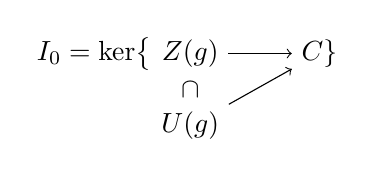
\begin{tikzpicture}[baseline=(z.base)]
\node (i) at (-1.22,0) {$I_0=\ker\bigl\{$};
\node (z) at (0,0) {$Z(\mathfrak g)$};
\node (c) at (1.64,0) {$\mathbb C\}$};
\node (u) at (0,-0.92) {$U(\mathfrak g)$};
\node at (0,-0.46) {$\cap$};
\draw[->] (z) -- (c);
\draw[->] (u) -- (c);
\end{tikzpicture}}\endgroup
\par (24)\quad --- stand. unique one-dim. character}
\end{GelfandAdjacentEvidence}
\begin{GelfandAdjacentEvidence}{GELFAND-P000932}{11}


$I_0$ --- Laplace operators without constant term

[crossed out: \sout{Assertion} (?)] \underline{Proposition}.
\Unclear{GELFAND-P000932}{before25-cancel}{The crossed-out word before “Proposition” resembles “Assertion”.}
\end{GelfandAdjacentEvidence}
\begin{GelfandAdjacentEvidence}{GELFAND-P000932}{12}


(25)\quad \underline{$D_X$-modules} $\Leftrightarrow$ \underline{representations} $\mathfrak g$,
\underline{on which there acts trivially} $I_0$.

($Z(\mathfrak g)$ must act as on the triv. one-dimensional representation)

\underline{Example (*).}

(26)\quad On $\mathbb P^1$ there are [inserted above: diff.] op.
\SourceFigure{GELFAND-P000932}{projective-operators}{A bracket underneath groups the three operators in (26). A curved leader joins the inserted “diff.” to “op.”.%
\par\smallskip
\begingroup\color{black}\GelfandFitDiagram{\begin{tikzpicture}
\node (operators) {$\dfrac{d}{dx},\quad x\dfrac{d}{dx}\quad\text{and}\quad x^2\dfrac{d}{dx}$};
\draw (operators.south west) -- ++(0,-0.12) -| (operators.south east);
\end{tikzpicture}}\endgroup}
\end{GelfandAdjacentEvidence}
\begin{GelfandAdjacentEvidence}{GELFAND-P000932}{13}

Take polynomials in them. This is the enveloping alg.

There is a unique op. commuting with all of them. (Shvartsman?)
\Unclear{GELFAND-P000932}{last-name}{The surname is tentatively read as Shvartsman. The question mark is in the manuscript.}
\end{GelfandAdjacentEvidence}


\underline{Moral:} representation theory reduces to the theory of $\mathcal D_X$-modules.

\underline{Improvement over what was known:} one can localize!!

\Needspace{7\baselineskip}
\begin{GelfandAdjacentEvidence}{GELFAND-P000933}{1}
\SourcePage{GELFAND-P000933}{unlabelled}

\underline{\underline{10.11.80}}\qquad\underline{Gelfand Sem.}
\Unclear{GELFAND-P000933}{above-date-marks}{There are several isolated strokes above the date. No letters or digits can be distinguished.}
\end{GelfandAdjacentEvidence}
\begin{GelfandAdjacentEvidence}{GELFAND-P000933}{2}


\underline{I. M. G.}\qquad\underline{\underline{Cayley numbers.}}
\begin{equation*}
 \left|\sum_{j=1}^{8}x_j e_j\right|=\sqrt{\sum_{1}^{8}x_j^2}
 \tag{1}
\end{equation*}
\Unclear{GELFAND-P000933}{formula1-overwritten-number}{A heavily overwritten or crossed-out stroke appears to the left of the digit in (1). The earlier mark is unresolved.}
\end{GelfandAdjacentEvidence}
\begin{GelfandAdjacentEvidence}{GELFAND-P000933}{3}

\Unclear{GELFAND-P000933}{right-sum-upper-limit}{The upper limit under the radical touches its bar. It is tentatively read as $8$ by comparison with the left side.}
\end{GelfandAdjacentEvidence}
\begin{GelfandAdjacentEvidence}{GELFAND-P000933}{4}


In the Cayley numbers:
\begin{equation*}
 |ab|=|a||b|
 \tag{2}
\end{equation*}

How to prove there are no $>8$ dim.?

From (2) one gets a problem in repr. theory and an explicit construction.

\underline{Question:} \uwave{perhaps it exists in an $\infty$-dimensional space?} (with cond. (2))

Gindikin asserts that it does. We must repeat the proof that in the finite-dimensional case there are none besides $\mathbb R,\mathbb C,\mathbb H$ and Cayley.

Projective geometries (planes).

Introduce coord., associativity $\Leftrightarrow$ Desarguesian property

The Cayley proj. plane is the simplest \uwave{non-Desarguesian one}

It is interesting to study differ. and locally homogeneous proj. planes.

--- The prob. of classifying Lie algebras is too particular (there should be no fragments

\hfill $G_2,E_6,E_7,E_8$ etc.
\SourceFigure{GELFAND-P000933}{exceptional-types}{The list of types is written below “there should be no fragments”. No closing parenthesis is visible.}
\end{GelfandAdjacentEvidence}
\begin{GelfandAdjacentEvidence}{GELFAND-P000933}{5}


\underline{\underline{Beilinson.}}\qquad\underline{On localization of representations.}

$X$ --- alg. variety (over $\mathbb C$),

$\mathcal A$ --- quasi-coherent $O_X$-module

\hspace{2em}\(\vert\) a sheaf of rings containing $O_X$.
\SourceFigure{GELFAND-P000933}{sheaf-vertical-mark}{A short vertical stroke descends from $\mathcal A$ to the next line.}
\end{GelfandAdjacentEvidence}
\begin{GelfandAdjacentEvidence}{GELFAND-P000933}{6}


(the inclusion $O_X\subset\mathcal A$ [inserted below: is given])
\SourceFigure{GELFAND-P000933}{inclusion-insertion}{“Is given” is inserted beneath the inclusion sign.}
\end{GelfandAdjacentEvidence}


(E.g., $\mathcal A$ is a sheaf of diff. operators)

\uwave{$\mathcal A$-mod} --- \uwave{the category of sheaves of left} $\mathcal A$-\uwave{mod.},
\uwave{that are quasi-coherent} $O_X$-\uwave{modules}

\Needspace{7\baselineskip}
\begin{GelfandAdjacentEvidence}{GELFAND-P000934}{1}
\SourcePage{GELFAND-P000934}{20}

(Last time $\mathcal A$ was diff. op.)

$A=\Gamma(\mathcal A)$,\qquad $A$-mod --- categ. of $A$-modules (left).

There are 2 adj. functors.
\SourceFigure{GELFAND-P000934}{adjunction-arrows}{In (1) the $\Gamma$ arrow points right, with the curved $\Delta$ arrow pointing left below it.%
\par\smallskip
\begingroup\color{black}\GelfandFitDiagram{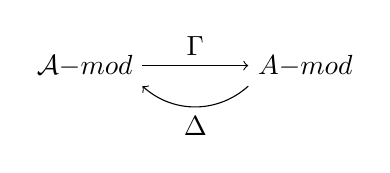
\begin{tikzpicture}[baseline=(sheaves.base)]
\node (sheaves) at (0,0) {$\mathcal A\text{-mod}$};
\node (modules) at (2.8,0) {$A\text{-mod}$};
\draw[->] (sheaves.east) -- node[above] {$\Gamma$} (modules.west);
\draw[->] (modules.south west) to[bend left=42] node[below] {$\Delta$} (sheaves.south east);
\end{tikzpicture}}\endgroup
\par (1)}
\end{GelfandAdjacentEvidence}
\begin{GelfandAdjacentEvidence}{GELFAND-P000934}{2}


\begin{equation*}
 \Delta(M)=\mathcal A\mathbin{\underset{A}{\otimes}}M,
 \tag{2}
\end{equation*}
$M$ is consid. as a const. sheaf of $\mathcal A$-mod. over $X$
(stalk $=M$ at each point) and the maps are trivial.
\SourceFigure{GELFAND-P000934}{tensor-over-A}{In (2) $A$ is written directly beneath the tensor sign.}
\end{GelfandAdjacentEvidence}
\begin{GelfandAdjacentEvidence}{GELFAND-P000934}{3}

\SourceFigure{GELFAND-P000934}{constant-module-notation}{A calligraphic $\mathcal A$ precedes “mod. over $X$”, as on the left in (1).}
\end{GelfandAdjacentEvidence}
\begin{GelfandAdjacentEvidence}{GELFAND-P000934}{4}


It is easy to see that they are adjoint.

(3)\quad \underline{Defn.-lemma.} [crossed out: \sout{a)} (?)]
\Unclear{GELFAND-P000934}{definition-cancel}{The sign after the heading is crossed out. It may be “a)”.}
\end{GelfandAdjacentEvidence}
\begin{GelfandAdjacentEvidence}{GELFAND-P000934}{5}


\uwave{A variety} $X$ \uwave{is called} $\mathcal A$-\uwave{affine}, \uwave{if one of the 2 equiv. conditions holds}

a)\enspace $\forall\,\mathcal M\in\mathcal A\text{-mod},\quad H^i(X,\mathcal M)=0,\quad i>0$ and
\[
 \begin{gathered}
 H^0(X,\mathcal M)\ne0\\[-2pt]
 \text{when }\mathcal M\ne0
 \end{gathered}
\]

b)\enspace \uwave{The functors} $\Gamma$ and $\Delta$ \uwave{are mutually inverse equivalences of categories}.

(In fact a) is equiv. to what we had last time, we change the modules)

a) is what we need to check, b) is what we need to use.
\SourceFigure{GELFAND-P000934}{need-check}{The same word, “need”, is written before both “check” and “use”.}
\end{GelfandAdjacentEvidence}
\begin{GelfandAdjacentEvidence}{GELFAND-P000934}{6}


\underline{Proof of the equivalence of a) and b).}

\underline{a) $\Rightarrow$ b).}
\begin{equation*}
 \Gamma(\mathcal M)=\operatorname{Hom}_{\mathcal A\text{-mod}}(\mathcal A,\mathcal M)
 \tag{4}
\end{equation*}
(the image of $1$ is a section of $\mathcal M$).

(5)\quad a) $\Rightarrow$ $\mathcal A$ --- a projective generator in the categ. $\mathcal A$-mod.

(6)\quad (an object such that i) $\operatorname{Hom}(\mathcal A,\mathcal M)$ --- \underline{exact} functor

(7)\quad ii) $\forall$ nonzero object $\mathcal M$;\enspace
$\operatorname{Hom}(\mathcal A,\mathcal M)\ne0$)

(i) follows from acyclicity, and ii) from the 2nd condition)

(exact functor --- takes exact seq. to exact ones)
\Unclear{GELFAND-P000934}{above-exact}{A detached vertical stroke stands above the end of “exact”. It may be an exclamation mark.}
\end{GelfandAdjacentEvidence}
\begin{GelfandAdjacentEvidence}{GELFAND-P000934}{7}


i)\enspace --- the property of projectivity

ii)\enspace --- generator

(by the way, ii) $\Rightarrow$ we can map $\mathcal A$ to the quotient $\mathcal M/\operatorname{Im}t$ and so on)
\SourceFigure{GELFAND-P000934}{quotient-symbol}{The symbol after $\operatorname{Im}$ in the denominator reads $t$.}
\end{GelfandAdjacentEvidence}
\begin{GelfandAdjacentEvidence}{GELFAND-P000934}{8}


(8)\quad iii) $\Gamma$ takes direct sums to direct sums.
\[
 \Gamma(\oplus_i\mathcal M_i)=\oplus\Gamma(\mathcal M_i)
\]
\Unclear{GELFAND-P000934}{direct-sum-index}{A small stroke beside the left direct-sum sign is tentatively read as an index $i$. There is no visible counterpart at the right sign.}
\end{GelfandAdjacentEvidence}


\Needspace{7\baselineskip}
\begin{GelfandAdjacentEvidence}{GELFAND-P000935}{1}
\SourcePage{GELFAND-P000935}{unlabelled}

(a property of all quasi-coh. sheaves)

\underline{General categorical fact}

(9)\quad \underline{Lemma.} Let there be given $\forall$ category $C$ (abelian)
[inserted above: with direct sums in $\forall$ quantity.], $X\in C$,
\SourceFigure{GELFAND-P000935}{direct-sums-insert}{A leader from “(abelian)” points to the insertion about direct sums.}
\end{GelfandAdjacentEvidence}
\begin{GelfandAdjacentEvidence}{GELFAND-P000935}{2}


$X$ --- Proj. generator with property (8):
\Unclear{GELFAND-P000935}{overwritten-X}{The $X$ at the start of the line is heavily retraced. The writing underneath is unresolved.}
\end{GelfandAdjacentEvidence}
\begin{GelfandAdjacentEvidence}{GELFAND-P000935}{3}


(10)\quad $\operatorname{Hom}_C(X,\cdot)$ commutes with direct sums.

(11)\quad [crossed out: \sout{Then}]
\[
 \operatorname{Hom}_C(X,\cdot):C\longrightarrow\operatorname{End}_C X\text{-mod}
\]
\SourceFigure{GELFAND-P000935}{crossed-then}{“Then” is crossed out before formula (11).}
\end{GelfandAdjacentEvidence}
\begin{GelfandAdjacentEvidence}{GELFAND-P000935}{4}


Then this functor is an \uwave{equiv. of categories}.

Everything follows from the lemma if we apply it to the case where
\begin{equation*}
 C=\mathcal A\text{-mod},\quad X=\mathcal A,\quad\operatorname{End}_C X=A
 \tag{12}
\end{equation*}
\SourceFigure{GELFAND-P000935}{endomorphism-ring}{The right side of (12) reads $\operatorname{End}_C X=A$.}
\end{GelfandAdjacentEvidence}
\begin{GelfandAdjacentEvidence}{GELFAND-P000935}{5}


The conv. implication \underline{b) $\Rightarrow$ a)} \underline{from} the Čech resolution.

$\mathcal D$-affine variety, a variety that is $\mathcal A$-aff. for $\mathcal A=\mathcal D_X$.

(13)\quad \underline{Thm.} $\mathbb P^N$ --- $\mathcal D$-\uwave{affine}.

The following theorem:
\SourceFigure{GELFAND-P000935}{theorem-heading}{The heading begins with “Следующая”, meaning “The following”.}
\end{GelfandAdjacentEvidence}
\begin{GelfandAdjacentEvidence}{GELFAND-P000935}{6}


$G$ --- a reductive group.

$X=G/B$ --- flag space

($B$ --- Borel subgroup)

(14)\quad $x\in X\Rightarrow\underset{\text{(stab.)}}{B_x}$ --- the corresp. Borel subgroup
\SourceFigure{GELFAND-P000935}{stabilizer-note}{“(stab.)” is inserted beneath $B_x$.}
\end{GelfandAdjacentEvidence}
\begin{GelfandAdjacentEvidence}{GELFAND-P000935}{7}


$G$ --- acts on $X\Rightarrow\mathfrak g$ acts on $X$.
\begin{equation*}
 \mathfrak g\longrightarrow\operatorname{Vect}X
 \tag{15}
\end{equation*}
\Unclear{GELFAND-P000935}{overwritten-15}{The second digit in (15) is heavily retraced and reads $5$.}
\end{GelfandAdjacentEvidence}
\begin{GelfandAdjacentEvidence}{GELFAND-P000935}{8}


hence.
\begin{equation*}
 U(\mathfrak g)\longrightarrow D_X=\Gamma(\mathcal D_X).
 \tag{16}
\end{equation*}

\SourceFigure{GELFAND-P000935}{center-leader}{A short hooked stroke under $Z(\mathfrak g)$ stands next to the label “center”.%
\par\smallskip
\begingroup\color{black}\GelfandFitDiagram{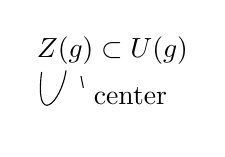
\begin{tikzpicture}[baseline=(z.base)]
\node (z) at (0,0) {$Z(\mathfrak g)\subset U(\mathfrak g)$};
\draw (-0.9,-0.27) .. controls (-0.99,-0.98) and (-0.65,-0.67) .. (-0.59,-0.25);
\draw (-0.40,-0.32) -- (-0.37,-0.47);
\node[anchor=west] at (-0.36,-0.58) {center};
\end{tikzpicture}}\endgroup
\par (17)}
\end{GelfandAdjacentEvidence}
\begin{GelfandAdjacentEvidence}{GELFAND-P000935}{9}


$I$ --- the annihilator of the unit repr. [?]
\Unclear{GELFAND-P000935}{annihilator-final-symbol}{The last sign after “repr.” is overwritten. The exact reading is unresolved.}
\end{GelfandAdjacentEvidence}
\begin{GelfandAdjacentEvidence}{GELFAND-P000935}{10}


(max ideal in the center)
\begin{equation*}
 J=I\cdot U(\mathfrak g).
 \tag{18}
\end{equation*}

(19)\quad \underline{Theorem.} a) $X$ --- $\mathcal D$-\uwave{affine}.

b)\enspace \uwave{under the morphism} (16) \uwave{one obtains an isomorphism}
\begin{equation*}
 U(\mathfrak g)/J\overset{\sim}{\longrightarrow}D_X
 \tag{20}
\end{equation*}
\SourceFigure{GELFAND-P000935}{isomorphism-arrow}{In (20) a single arrow has a tilde above it.}
\end{GelfandAdjacentEvidence}


(21)\quad hence, equiv. of the categories of 1) $\mathcal D$-sheaves on $X$ and 2) representations of the Lie alg. $\mathfrak g$ with unit infinitesim. character.

\Needspace{7\baselineskip}
\begin{GelfandAdjacentEvidence}{GELFAND-P000936}{1}
\SourcePage{GELFAND-P000936}{21}

[crossed out: \sout{Definition} (?)]\qquad\underline{Digression.}
\Unclear{GELFAND-P000936}{cancelled-heading}{The crossed-out heading resembles “Definition”. The exact reading is unresolved.}
\end{GelfandAdjacentEvidence}
\begin{GelfandAdjacentEvidence}{GELFAND-P000936}{2}

\SourceFigure{GELFAND-P000936}{section-heading}{The new heading reads “Отступление”, or “Digression”.}
\end{GelfandAdjacentEvidence}
\begin{GelfandAdjacentEvidence}{GELFAND-P000936}{3}


$X,Y$ --- both smooth alg. varieties.
\SourceFigure{GELFAND-P000936}{opening-word}{The word after $X,Y$ reads “both”.}
\end{GelfandAdjacentEvidence}
\begin{GelfandAdjacentEvidence}{GELFAND-P000936}{4}


$X\overset f\longrightarrow Y$ a map.

Then there are the categories $\mathcal D_X\text{-mod}$ and $\mathcal D_Y\text{-mod}$

There are 2 functors on sheaves $f^*$ and $f_*$.

But in diff. op. there is no corresp. morphism.

But the (natural) functors do exist, they are def. at the level of the derived category

(actually there are \uwave{4 functors})

(22)\quad $f^\circ$ --- inverse image in the cat. of \underline{\underline{sheaves}}.
\begin{equation*}
 O_X\mathbin{\underset{f^\circ O_Y}{\otimes}} f^\circ(\mathcal D_Y)
 \tag{23}
\end{equation*}
\SourceFigure{GELFAND-P000936}{inverse-image-23}{In (23) the marks above $f$ look like small hollow circles, as in (22).}
\end{GelfandAdjacentEvidence}
\begin{GelfandAdjacentEvidence}{GELFAND-P000936}{5}


\begin{equation*}
 \mathcal D_{X\to Y}\underset{\mathrm{def}}{=}
 O_X\mathbin{\underset{f^\bullet O_Y}{\otimes}} f^\bullet\mathcal D_Y
 \tag{24}
\end{equation*}
\SourceFigure{GELFAND-P000936}{inverse-image-24}{In (24) the marks above both occurrences of $f$ are filled dots.}
\end{GelfandAdjacentEvidence}
\begin{GelfandAdjacentEvidence}{GELFAND-P000936}{6}


\begin{equation*}
 \mathcal D_{X\to Y}\text{ --- }
 \left\{\begin{array}{l}
 \text{left } \mathcal D_X\text{-module}\\
 \text{right } f^\circ\mathcal D_Y\text{-module}
 \end{array}\right.
 \tag{25}
\end{equation*}
\SourceFigure{GELFAND-P000936}{transfer-bimodule}{In the lower line of (25) the mark above $f$ has an open center.}
\end{GelfandAdjacentEvidence}
\begin{GelfandAdjacentEvidence}{GELFAND-P000936}{7}


left $\mathcal D_X$ by the Leibniz rule; rem. for vec. fields on $X$:
\SourceFigure{GELFAND-P000936}{leibniz-abbreviation}{After the semicolon the manuscript has the abbreviation «ост.» (“rem.”).}
\end{GelfandAdjacentEvidence}
\begin{GelfandAdjacentEvidence}{GELFAND-P000936}{8}


$v\in\operatorname{Vect}X$;
\[
 (df)(v)\in\Gamma(f^*T\,Y)
\]
\SourceFigure{GELFAND-P000936}{tangent-notation}{After $f^*$, $T$ and $Y$ are written on the same line.}
\end{GelfandAdjacentEvidence}
\begin{GelfandAdjacentEvidence}{GELFAND-P000936}{9}


$(df)(v)$ acts on \underline{\underline{$f^\bullet\mathcal D_Y$}}.
\Unclear{GELFAND-P000936}{final-left-mark}{A heavy slanted stroke stands to the left of the last line. There is no visible separate dot below it.}
\end{GelfandAdjacentEvidence}
\begin{GelfandAdjacentEvidence}{GELFAND-P000936}{10}

\SourceFigure{GELFAND-P000936}{last-inverse-image}{A filled dot stands above $f$. The expression is double underlined.}
\end{GelfandAdjacentEvidence}


\Needspace{7\baselineskip}
\begin{GelfandAdjacentEvidence}{GELFAND-P000937}{1}
\SourcePage{GELFAND-P000937}{unlabelled}

\underline{\underline{17.11.80}}\qquad\underline{Gelfand Sem.}

\underline{I. M. G.}\qquad\underline{problems.}

1.\quad
\[
 f(x)=\left\{\begin{array}{ll}
 1/q,&x=p/q\text{ --- in lowest terms}\\
 0,&x\text{ --- irrat.}
 \end{array}\right.
\]

Where is it continuous?

where is it differentiable?
\[
 f(x)=\left\{\begin{array}{ll}
 1/q^\alpha,&x=p/q\text{ --- in lowest terms}\\
 0,&x\text{ --- irrat.}
 \end{array}\right.
\]

What can be said about diff.?

2.\quad $f(x)=\lim\limits_{n\to\infty}\lim\limits_{m\to\infty}(\cos^{2m}2\pi n!x)$ --- the Dirichlet fn.
\SourceFigure{GELFAND-P000937}{dirichlet-limits}{The $n$ in the cosine argument is followed by a factorial sign. The inner limit is over $m$.}
\end{GelfandAdjacentEvidence}
\begin{GelfandAdjacentEvidence}{GELFAND-P000937}{2}


3.\quad Can the Dirichlet fn. be constructed with one limit sign?

(from cont. fns.)

[at upper right]

4.\quad Calculate approximately
\[
 \int_{-\infty}^{\infty}e^{-x^2}\cos1000x\,dx
\]

The same with $e^{-x^4}$ or $e^{-x^6}$
\SourceFigure{GELFAND-P000937}{upper-right-exercise}{Problem 4 is written in the upper right. The integral has $1000x$.}
\end{GelfandAdjacentEvidence}
\begin{GelfandAdjacentEvidence}{GELFAND-P000937}{3}


\underline{A. Beilinson.}

$X\overset f\longrightarrow Y$,\qquad $X,Y$ --- varieties.

$\mathcal D_X\text{-mod},\ \mathcal D_Y\text{-mod}$ --- categories of quasi-coher. sheaves of
$\mathcal D_X\text{-mod}$ and $\mathcal D_Y\text{-mod}$ on $X$ and $Y$
\SourceFigure{GELFAND-P000937}{functor-arrows}{The upper arrow points right and the lower arrow points left. The arrows carry no labels.%
\par\smallskip
\(\mathcal D_X\text{-mod}\ \substack{\longrightarrow\\\longleftarrow}\
\mathcal D_Y\text{-mod}\)\par functors}
\end{GelfandAdjacentEvidence}
\begin{GelfandAdjacentEvidence}{GELFAND-P000937}{4}


Let us define:
\[
 f^*:\mathcal D_Y\text{-mod}\longrightarrow\mathcal D_X\text{-mod}
\]
\begin{equation*}
 f^*(\mathcal M)=O_X\mathbin{\underset{f^\bullet(O_Y)}{\otimes}}
 f^\bullet(\mathcal M),\qquad \mathcal M\in\mathcal D_Y\text{-mod}
 \tag{1}
\end{equation*}

(as a sheaf --- \uwave{inverse image in the categ. of} $O$-\uwave{modules},
$f^\bullet$ --- the abstract inverse image)
\SourceFigure{GELFAND-P000937}{pullback-dots}{Both occurrences of $f$ on the right of (1) have filled dots. The star is on the left.}
\end{GelfandAdjacentEvidence}
\begin{GelfandAdjacentEvidence}{GELFAND-P000937}{5}


Action of diff. operators: vec. fields suffice $v\in\operatorname{Vect}X$,
\begin{equation*}
 \ell\otimes m\in f^*(\mathcal M)
 \tag{2}
\end{equation*}
\SourceFigure{GELFAND-P000937}{tensor-factor-leaders}{Two leaders appear below the factors in (2).%
\par\smallskip
\begingroup\color{black}\GelfandFitDiagram{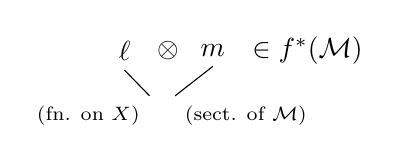
\begin{tikzpicture}[baseline=(l.base)]
\node (l) at (0,0) {$\ell$};
\node at (0.55,0) {$\otimes$};
\node (m) at (1.12,0) {$m$};
\node[anchor=west] at (1.5,0) {$\in f^*(\mathcal M)$};
\node (fn) at (-0.46,-0.82) {\scriptsize (fn. on $X$)};
\node (sect) at (1.54,-0.82) {\scriptsize (sect. of $\mathcal M$)};
\draw (l.south) -- (fn.north east);
\draw (m.south) -- (sect.north west);
\end{tikzpicture}}\endgroup}
\end{GelfandAdjacentEvidence}
\begin{GelfandAdjacentEvidence}{GELFAND-P000937}{6}


\begin{equation*}
 df(v)=\sum
 \underset{\substack{\vert\\\text{fn. on }X}}{\tau_i}
 \otimes\frac{\partial}{\partial y_i}\in f^*(T_Y),
 \qquad df:T_X\longrightarrow f^*T_Y
 \tag{3}
\end{equation*}
\SourceFigure{GELFAND-P000937}{tau-leader}{The note under $\tau_i$ reads “fn. on $X$” in the singular.}
\end{GelfandAdjacentEvidence}
\begin{GelfandAdjacentEvidence}{GELFAND-P000937}{7}


Instead of (1), one can write more simply
\begin{equation*}
 f^*(\mathcal M)=O_X\mathbin{\underset{O_Y}{\otimes}}\mathcal M
 \tag{4}
\end{equation*}
In this same sense:
\begin{equation*}
 f^*(T_Y)=O_X\mathbin{\underset{O_Y}{\otimes}}T_Y
 \tag{5}
\end{equation*}
\begin{equation*}
 v\cdot(\ell\otimes m)\underset{\mathrm{def}}{=}
 v(\ell)\otimes m+\sum\ell\tau_i\otimes\frac{\partial}{\partial y_i}m
 \tag{6}
\end{equation*}
(by the Leibniz formula).
\SourceFigure{GELFAND-P000937}{leibniz-action}{The equality in (6) has $\mathrm{def}$ below it. The coefficient in the sum reads $\ell\tau_i$.}
\end{GelfandAdjacentEvidence}


\Needspace{7\baselineskip}
\begin{GelfandAdjacentEvidence}{GELFAND-P000938}{1}
\SourcePage{GELFAND-P000938}{24}

If $\mathcal M$ comes from a vec. bundle with an integr. [inserted below: (flat)] connection, then this is the usual inverse image of the connection.
\SourceFigure{GELFAND-P000938}{flat-insert}{“(Flat)” is inserted beneath “integr.”.}
\end{GelfandAdjacentEvidence}
\begin{GelfandAdjacentEvidence}{GELFAND-P000938}{2}


(7)\quad \underline{Examples.}

1.\enspace $f^*O_Y=O_X$

2.\enspace From a sheaf [crossed out: unresolved sign] of fin. type there may result [inserted above: a sheaf] of infinite type
\Incomplete{GELFAND-P000938}{example-two-cancel}{The sign after “sheaf” is heavily crossed out. It may be $\mathcal D$.}
\end{GelfandAdjacentEvidence}
\begin{GelfandAdjacentEvidence}{GELFAND-P000938}{3}

\SourceFigure{GELFAND-P000938}{sheaf-insert}{“Sheaf” is inserted above the line with a leader.}
\end{GelfandAdjacentEvidence}
\begin{GelfandAdjacentEvidence}{GELFAND-P000938}{4}


$X$ --- a point, $Y$ --- a var..
\SourceFigure{GELFAND-P000938}{example-two-manifold}{The abbreviation after $Y$ reads «мн-зие» (“var.”).}
\end{GelfandAdjacentEvidence}
\begin{GelfandAdjacentEvidence}{GELFAND-P000938}{5}


$f^*(\mathcal D_Y)$ is infinite-dimensional (as a vec. space)
\[
 \mathcal D_X=\mathbb C
\]
$f^*(\mathcal D_Y)$ --- diff. op. with const. coefficients

3.\enspace $X,Y$ as above, $\mathcal M$ --- $\delta$-fns. at the point $X\in Y$
$\underset{\mathrm{def}}{=}\delta_x$

(generalized fns. concentr. at a point).

Then
\[
 f^*(\delta_x)=0,
\]
since $\forall$ generalized fn. [inserted above: at a pt.] can be repres. in the form
\[
 \sum \alpha_i s_i,\qquad \alpha_i(X)=0.
\]
\SourceFigure{GELFAND-P000938}{point-insert}{“At a pt.” is inserted above the line with a leader.}
\end{GelfandAdjacentEvidence}
\begin{GelfandAdjacentEvidence}{GELFAND-P000938}{6}


\SourceFigure{GELFAND-P000938}{delta-arrows}{An arrow leads from $y$ to $0$, and one from $\delta'(y)$ to “?”.%
\par\smallskip
\begingroup\color{black}\GelfandFitDiagram{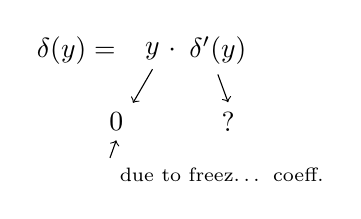
\begin{tikzpicture}[baseline=(ly.base)]
\node (ly) at (0,0) {$\delta(y)={}$};
\node (y) at (0.92,0) {$y$};
\node at (1.17,0) {$\cdot$};
\node (deriv) at (1.75,0) {$\delta'(y)$};
\node (zero) at (0.46,-0.90) {$0$};
\node (q) at (1.88,-0.90) {?};
\node[anchor=west] (reason) at (0.38,-1.57) {\scriptsize due to freez… coeff.};
\draw[->] (y.south) -- (zero.north east);
\draw[->] (deriv.south) -- (q.north);
\draw[->] (reason.north west) -- (zero.south);
\end{tikzpicture}}\endgroup}
\end{GelfandAdjacentEvidence}
\begin{GelfandAdjacentEvidence}{GELFAND-P000938}{7}

\SourceFigure{GELFAND-P000938}{delta-sign}{There is an equals sign with no visible minus before $y$.}
\end{GelfandAdjacentEvidence}
\begin{GelfandAdjacentEvidence}{GELFAND-P000938}{8}


\underline{Direct image} is def. for right mod. (integr. forms only!, and they are a right mod.)

\[
 f_*\quad\text{mod-}\mathcal D_X\longrightarrow\text{mod-}\mathcal D_Y
\]
(integr. the volume forms on $X$ [inserted below and circled: along the fibers] gives a volume form on $Y$)
\SourceFigure{GELFAND-P000938}{fiber-insert}{The insertion “along the fibers” is circled below the line.}
\end{GelfandAdjacentEvidence}
\begin{GelfandAdjacentEvidence}{GELFAND-P000938}{9}


\begin{equation*}
 \underset{\substack{\vert\\\text{a sheaf on }X}}{\mathcal D_{X\to Y}}
 = f^*(\mathcal D_Y)\in\mathcal D_X\text{-mod-}\mathcal D_Y
 \tag{8}
\end{equation*}
\SourceFigure{GELFAND-P000938}{sheaf-on-x}{A vertical leader extends down from the sheaf symbol in (8).}
\end{GelfandAdjacentEvidence}
\begin{GelfandAdjacentEvidence}{GELFAND-P000938}{10}


(a left $\mathcal D_X$-module and a right $\mathcal D_Y$-module)
\begin{equation*}
 f_*(\mathcal M)=f_{\cdot}\left(\mathcal M\mathbin{\underset{\mathcal D_X}{\otimes}}\mathcal D_{X\to Y}\right)
 \tag{9}
\end{equation*}
$f_{\cdot}$ --- direct image on sheaves

[crossed out: earlier number unresolved] (10)\quad \underline{Examples.}
\Unclear{GELFAND-P000938}{example-ten-cancel}{An earlier number is crossed out before (10). Its digit is unresolved.}
\end{GelfandAdjacentEvidence}
\begin{GelfandAdjacentEvidence}{GELFAND-P000938}{11}


1.\enspace $X=x\in Y$. Consid. the stand. 1-dim. $\mathcal D_X$-module $(=\mathbb C)$
\SourceFigure{GELFAND-P000938}{standard-abbreviation}{The abbreviation before “1-dim.” reads “stand.”.}
\end{GelfandAdjacentEvidence}
\begin{GelfandAdjacentEvidence}{GELFAND-P000938}{12}

\[
 f_*(\mathcal M)\text{ --- (generalized fns. concentr. at the point on }Y\text{)}=\delta_x
\]
\[
 f^*(\mathcal D_Y)=\mathcal D_Y/\sum y_iD_Y
\]
\SourceFigure{GELFAND-P000938}{quotient-D}{The $D$ in the denominator appears plain, without the calligraphic flourish of the numerator.}
\end{GelfandAdjacentEvidence}
\begin{GelfandAdjacentEvidence}{GELFAND-P000938}{13}


[at right] Freez… (?) coeff. $=$ applying an op. to the $\delta$-fn..
\Unclear{GELFAND-P000938}{freeze-coefficients}{The start of the word is tentatively read as “freez…”. The exact ending is unresolved.}
\end{GelfandAdjacentEvidence}


($\Rightarrow\mathcal D_Y$-module)

\Needspace{7\baselineskip}
\begin{GelfandAdjacentEvidence}{GELFAND-P000939}{1}
\SourcePage{GELFAND-P000939}{unlabelled}

2.\enspace \underline{Let us generalize:}
\[
 X\overset f\longrightarrow Y\qquad\text{embedding}
\]
$f_*(\mathcal M)$ by defn. --- extension by means of $\delta$-fns. in the transv. direction.
\SourceFigure{GELFAND-P000939}{volume-forms-leader}{A short stroke beneath $\omega_X$ leads to the caption.%
\par\smallskip
\begingroup\color{black}\GelfandFitDiagram{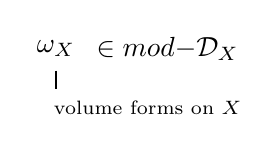
\begin{tikzpicture}[baseline=(w.base)]
\node (w) at (0,0) {$\omega_X$};
\node[anchor=west] at (0.39,0) {$\in\text{mod-}\mathcal D_X$};
\draw (0,-0.28) -- (0,-0.51);
\node[anchor=west] at (-0.15,-0.75) {\scriptsize volume forms on $X$};
\end{tikzpicture}}\endgroup}
\end{GelfandAdjacentEvidence}
\begin{GelfandAdjacentEvidence}{GELFAND-P000939}{2}


$f_*(\omega_X)$ --- generalized fns. concentr. on $X$ and smooth in the dir. of $X$.

3.\enspace more generally:

[crossed out: earlier number unresolved] Vector bundle with a right connection (in place of volume forms)
\Unclear{GELFAND-P000939}{upper-cancelled-number}{The crossed-out digit resembles $4$. The exact reading is unresolved.}
\end{GelfandAdjacentEvidence}
\begin{GelfandAdjacentEvidence}{GELFAND-P000939}{3}


[added below: twist. by volume forms]
\SourceFigure{GELFAND-P000939}{volume-twist}{“Twist. by volume forms” is added beneath the line about the connection.}
\end{GelfandAdjacentEvidence}
\begin{GelfandAdjacentEvidence}{GELFAND-P000939}{4}


\uwave{Relation to cohomology.}

[crossed out: earlier number unresolved] \uwave{$Y$ --- a point}, $X$ --- a var.
\Unclear{GELFAND-P000939}{middle-cancelled-number}{The earlier number before “$Y$ is a point” is crossed out. It may be $4$.}
\end{GelfandAdjacentEvidence}
\begin{GelfandAdjacentEvidence}{GELFAND-P000939}{5}


$f^*(\mathcal M)$ --- the sheaf of fns., rep. in the requisite number of copies.

$f_*$ here computes the cohomology of the space $X$.

\uwave{Higher direct images.}
\begin{equation*}
 \underset{\vert}{L} f^*:D\,D_Y\text{-mod}\longrightarrow D\,D_X\text{-mod}
 \tag{11}
\end{equation*}
left derived functor of $f^*$.
\SourceFigure{GELFAND-P000939}{left-derived-leader}{A vertical stroke below $L$ leads to the caption.}
\end{GelfandAdjacentEvidence}
\begin{GelfandAdjacentEvidence}{GELFAND-P000939}{6}


$D$ --- derived category

\SourceFigure{GELFAND-P000939}{right-derived-annotation}{Two slanted strokes beneath the integral sign lead to “$R f_*$ (?)”.%
\par\smallskip
\begingroup\color{black}\GelfandFitDiagram{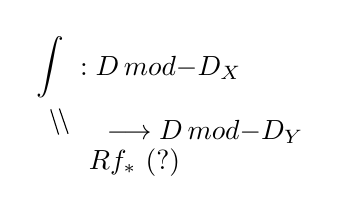
\begin{tikzpicture}[baseline=(int.base)]
\node (int) at (0,0) {$\displaystyle\int$};
\node[anchor=west] at (0.25,0) {$:D\,\text{mod-}D_X$};
\node[anchor=west] at (0.59,-0.82) {$\longrightarrow D\,\text{mod-}D_Y$};
\draw (0,-0.53) -- (0.10,-0.85);
\draw (0.11,-0.52) -- (0.22,-0.84);
\node[anchor=west] at (0.36,-1.20) {$R f_*\ (?)$};
\end{tikzpicture}}\endgroup
\par (12)}
\end{GelfandAdjacentEvidence}
\begin{GelfandAdjacentEvidence}{GELFAND-P000939}{7}


\begin{equation*}
 \int\mathcal M=R f_\bullet
 \left(\mathcal M\mathbin{\underset{D_X}{\overset L\otimes}}\mathcal D_{X\to Y}\right)
 \qquad\text{--- a complex}
 \tag{13}
\end{equation*}
\Unclear{GELFAND-P000939}{equation-thirteen-cancelled-subscript}{An $X$ appears below $D$. The earlier sign crossed out beside it is unresolved.}
\end{GelfandAdjacentEvidence}
\begin{GelfandAdjacentEvidence}{GELFAND-P000939}{8}

\begin{equation*}
 \int^i\mathcal M=H^i\left(\int\mathcal M\right)
 \tag{14}
\end{equation*}
(Sato, Kashiwara)

(15)\quad \underline{Theorem.} $Y$ --- a point $\Rightarrow$
\begin{equation*}
 \int^i\omega_X=H^{\dim X+i}(X)
 \tag{16}
\end{equation*}
\SourceFigure{GELFAND-P000939}{last-formula-number}{The formula is numbered (16). The lower loop of the last digit is closed.}
\end{GelfandAdjacentEvidence}
\begin{GelfandAdjacentEvidence}{GELFAND-P000939}{9}

\Incomplete{GELFAND-P000939}{last-exponent-cancellation}{A sign is crossed out before $\dim X+i$ in the exponent. The exact reading is unresolved.}
\end{GelfandAdjacentEvidence}


($X$ --- nonsingular over $\mathbb C$)

\Needspace{7\baselineskip}
\begin{GelfandAdjacentEvidence}{GELFAND-P000940}{1}
\SourcePage{GELFAND-P000940}{25}

\underline{S. Gelfand}

\uwave{Derived category.}
\SourceFigure{GELFAND-P000940}{derived-title}{The heading has “category” in the singular.}
\end{GelfandAdjacentEvidence}
\begin{GelfandAdjacentEvidence}{GELFAND-P000940}{2}


\underline{Prob. 1.} If there are 2 compl. with isom. cohomologies, one cannot always extend an isom. of cohom. to a map of compl. inducing an isomorphism.

\underline{Prob. 2.} Consid. the sphere $S^n$ and on it the cat. of sheaves of ab. groups $C$. Acting on it is $O(n)$.
Consid. the cat. with the action of the grp. and the derived cat. $D(C)$. Consid. the dual $S^{*n}$. $C_1$ [crossed out: unresolved]
\SourceFigure{GELFAND-P000940}{top-action-abbreviation}{After “action” the abbreviation reads «гр.» (“grp.”).}
\end{GelfandAdjacentEvidence}
\begin{GelfandAdjacentEvidence}{GELFAND-P000940}{3}

\Incomplete{GELFAND-P000940}{top-cancelled-symbol}{A sign to the right of the first $C_1$ is heavily crossed out.}
\end{GelfandAdjacentEvidence}
\begin{GelfandAdjacentEvidence}{GELFAND-P000940}{4}


$C_1$ is not isom. to $C$ (the action is different)
\[
 \underline{\underline{D(S)\sim D(S^*)}}\quad!!
\]

\underline{24.11.80}\qquad\underline{Gelfand Sem.}

\uwave{Sectional sessions.}

\underline{25}\quad rm. \(\underrightarrow{451}\)\quad [crossed out: unresolved]
\Unclear{GELFAND-P000940}{section-room-prefix}{The abbreviation before 451 is tentatively read as «к.» (“rm.”).}
\end{GelfandAdjacentEvidence}
\begin{GelfandAdjacentEvidence}{GELFAND-P000940}{5}

\Incomplete{GELFAND-P000940}{section-cancelled-entry}{The crossed-out writing before $15^{00}$ is unresolved.}
\end{GelfandAdjacentEvidence}
\begin{GelfandAdjacentEvidence}{GELFAND-P000940}{6}


\begin{tabular}{@{}ll@{}}
$15^{\underline{00}}$ & Sergeev\\
$15^{\underline{20}}$ & \underline{Mebkhout} (France)\\
& Riem.-Hilb. prob. in higher dim.\\
$15^{\underline{40}}$ & Henkin\\
$16^{\underline{00}}$ & \underline{Kantor} J.-M.
\end{tabular}

[boxed at right]

\underline{Conf.}\qquad\underline{\underline{Plenary sessions.}}

\begin{tabular}{@{}lll@{}}
\underline{24.} & $16^{\underline{20}}$ & Sato\\
\underline{25} & $10^{\underline{00}}$ & Morimoto\\
 & $10^{\underline{40}}$ & Maslov\\
 & $11^{\underline{40}}$ & Gesztelyi\\
 & & (generalized fns. in eqs. partial (?)\\
 & $12^{\underline{20}}$ & Berezanskii et al.
\end{tabular}
\Unclear{GELFAND-P000940}{gesztelyi-note-ending}{The ending after «в ур.» is tentatively read as «частн.» (“partial”). No closing parenthesis is visible.}
\end{GelfandAdjacentEvidence}
\begin{GelfandAdjacentEvidence}{GELFAND-P000940}{7}


\begin{tabular}{@{}lll@{}}
\underline{26.} & [crossed out: unresolved]\quad\underline{10.00} & \underline{Laugwitz}\\
 & & (from a nonstand. point of view)\\
 & $10^{\underline{40}}$ & \underline{Ivanov}\\
 & $11^{\underline{40}}$ & \underline{Khromov}, \underline{Danilov}\\
 & $12^{\underline{20}}$ & \underline{Berg}\quad multiplic. of distrib.
\end{tabular}
\Incomplete{GELFAND-P000940}{conference-cancelled-time}{The earlier time before 10.00 is heavily crossed out.}
\end{GelfandAdjacentEvidence}
\begin{GelfandAdjacentEvidence}{GELFAND-P000940}{8}


\begin{tabular}{@{}lll@{}}
\underline{28.} & $10^{\underline{00}}$ & \underline{Lions}\\
 & $10^{\underline{40}}$ & \underline{Gelfand}\\
 & $11^{\underline{40}}$ & \underline{Komatsu} --- kernels in ultradistrib.\\
 & $12^{\underline{20}}$ & \underline{Lassner}\\
 & $13^{\underline{00}}$ & \underline{Zharinov}
\end{tabular}

\underline{D. B. Fuchs.}\qquad\underline{Whitehead mult.}
\[
 \pi_n(X)\times\pi_m(X)\longrightarrow\pi_{n+m}(X)
\]
$\sim$ commutator in a Lie alg.
\[
 \partial(I_n\times I_m)=(\partial I_n\times I_m)\cup(I_n\times\partial I_m)
\]
There is a Jacobi identity --- Lie supersym.!!
\SourceFigure{GELFAND-P000940}{fuchs-final-abbreviation}{The abbreviation before “Lie” reads «суперсим.» (“supersym.”).}
\end{GelfandAdjacentEvidence}
\begin{GelfandAdjacentEvidence}{GELFAND-P000940}{9}


\underline{\underline{V. Lomonosov.}}

$(A-A')$ --- nuclear

$B$ comm. with $A$, $B$ comm. with $A'$, $(B-B')$ --- compl. cont.
\SourceFigure{GELFAND-P000940}{lomonosov-second-B}{The $B$ before $A'$ has no visible prime.}
\end{GelfandAdjacentEvidence}
\begin{GelfandAdjacentEvidence}{GELFAND-P000940}{10}

\[
 \Rightarrow\quad B|_{\mathcal H_{ac}(B)}\underset{\text{unit.}}{\sim}
 B'|_{\mathcal H_{ac}(B')}
\]
$\Rightarrow$ the theor. is consid. directly for commut. families of operators.

\underline{\underline{A. Beilinson.}}

\(X\overset f\longrightarrow Y\)
\begin{equation*}
 f^*:\mathcal D_Y\text{-mod}\longrightarrow\mathcal D_X\text{-mod}
 \tag{1}
\end{equation*}
Introduce
\[
 f_*:\text{mod-}\mathcal D_X\longrightarrow\text{mod-}\mathcal D_Y
\]
[at right]
\[
 \left[\begin{aligned}
 &\text{if }\overset{\text{on $Y$}}{u}\text{ sat. the syst. }M,\\
 &\text{then }f^*u\text{ sat. the syst. }f^*M
 \end{aligned}\right.
\]
\SourceFigure{GELFAND-P000940}{upper-bracketed-note}{“On $Y$” is inserted above $u$ in the upper note on the right.}
\end{GelfandAdjacentEvidence}
\begin{GelfandAdjacentEvidence}{GELFAND-P000940}{11}


\begin{equation*}
 \mathcal D_{X\to Y}=f^*(\mathcal D_Y)\in\mathcal D_X\text{-mod-}\mathcal D_Y
 \qquad\text{(bimodule)}
 \tag{2}
\end{equation*}
\begin{equation*}
 f_*M=f_\bullet\left(M\mathbin{\underset{\mathcal D_X}{\otimes}}\mathcal D_{X\to Y}\right)
 \tag{3}
\end{equation*}
(\(\underset{\text{if}}{f_*}\) on volume forms of comp. support)

[at right]
\[
 \left[\begin{aligned}
 &\text{if }u\ \overset{\in\Omega_1(X)}{\text{on $X$}}\text{ sat. the syst. }M,\\
 &\text{then }f_*u\text{ sat. the syst. }f_*M
 \end{aligned}\right.
\]
\Unclear{GELFAND-P000940}{lower-right-omega-insertion}{The small subscript on $\Omega$ resembles $1$. The exact reading is unresolved.}
\end{GelfandAdjacentEvidence}
\begin{GelfandAdjacentEvidence}{GELFAND-P000940}{12}

\SourceFigure{GELFAND-P000940}{lower-bracketed-note}{The lower note on the right begins with an opening square bracket.}
\end{GelfandAdjacentEvidence}


\Needspace{7\baselineskip}
\begin{GelfandAdjacentEvidence}{GELFAND-P000941}{1}
\SourcePage{GELFAND-P000941}{unlabelled}

(System of eqs. satisfied by improper integrals)

(4)\quad $f_*$ is not functorial: \qquad $(fg)_*\ne f_*g_*$
\SourceFigure{GELFAND-P000941}{ordinary-composition}{In (4) $fg$ and $f_*g_*$ are written in this order.}
\end{GelfandAdjacentEvidence}
\begin{GelfandAdjacentEvidence}{GELFAND-P000941}{2}


Let us construct.
\begin{equation*}
 Rf_*:D(\text{mod-}D_X)\longrightarrow D(\text{mod-}D_Y)
 \tag{5}
\end{equation*}

\underline{Example:} $X$ --- a plane, $Y$ --- a line, $f$ --- projection,

$\mathcal M$ --- a sheaf of forms on $X$ (of top degree)
\[
 Rf_*(\mathcal M)\text{ --- a complex,}\qquad
 \begin{aligned}
 &0\text{-comp. --- }0\\
 &(-1)\text{-comp. --- }\text{\uwave{forms on the line.}}
 \end{aligned}
\]
\SourceFigure{GELFAND-P000941}{example-components}{The example gives the $0$-comp. and the $(-1)$-comp.}
\end{GelfandAdjacentEvidence}
\begin{GelfandAdjacentEvidence}{GELFAND-P000941}{3}


\begin{equation*}
 Rf_*(\mathcal M)=Rf_\bullet
 \left(\mathcal M\mathbin{\underset{\mathcal D_X}{\overset L\otimes}}\mathcal D_{X\to Y}\right)
 \tag{6}
\end{equation*}
$\overset L\otimes$ --- the left derived functor of the tens. product.

$Rf_\bullet$ --- the right derived functor of the functor (!) $f_\bullet$

(7)\quad \underline{Prop.}
\SourceFigure{GELFAND-P000941}{derived-composition}{A double arrow below the chain $X\to Y\to Z$ points down to the formula.%
\par\smallskip
\begingroup\color{black}\GelfandFitDiagram{\begin{tikzpicture}[baseline=(maps.base)]
\node (maps) at (0,0) {$X\overset f\longrightarrow Y\overset g\longrightarrow Z$};
\node at (0,-0.63) {$\Downarrow$};
\node at (0,-1.23) {$Rg_*Rf_*=R(g\circ f)_*$};
\end{tikzpicture}}\endgroup}
\end{GelfandAdjacentEvidence}
\begin{GelfandAdjacentEvidence}{GELFAND-P000941}{4}


[crossed out: \sout{(since}] ($f_*$ lacks this prop.)
\Unclear{GELFAND-P000941}{cancelled-word-before-parenthesis}{An opening parenthesis and the start of “since” are crossed out.}
\end{GelfandAdjacentEvidence}
\begin{GelfandAdjacentEvidence}{GELFAND-P000941}{5}


Let
\[
 \mathcal M\in\text{mod-}\mathcal D_X
\]
\begin{equation*}
 \ldots\longrightarrow\mathcal M\otimes\Lambda^2T_X
 \longrightarrow\mathcal M\otimes T_X\underset{\nearrow}{\longrightarrow}\mathcal M
 \tag{8}
\end{equation*}
($T_X$ --- tangent sheaf to $X$)\qquad (since $\mathcal M$ --- a right
 $\mathcal D_X\text{-mod},\ T_X\subset\mathcal D_X$)
\SourceFigure{GELFAND-P000941}{last-differential-leader}{An arrow from the right-hand note points toward the last differential in (8).}
\end{GelfandAdjacentEvidence}
\begin{GelfandAdjacentEvidence}{GELFAND-P000941}{6}


(9)\quad \underline{Prop.}

\uwave{Consid. the cohomology of} (8). \uwave{It agrees with the cohom. of the compl.} (6), i.e.

\hspace{2em}(de Rham!)
\begin{equation*}
 R\Gamma(\underbrace{DR}_{\text{De Rham}}\mathcal M)=Rf_*(\mathcal M)
 \tag{10}
\end{equation*}
(\uwave{here} $f:X\longrightarrow\text{\uwave{a point}}$).
\SourceFigure{GELFAND-P000941}{de-rham-underlabel}{Below $DR$ a bracket leads to the label “De Rham”.}
\end{GelfandAdjacentEvidence}
\begin{GelfandAdjacentEvidence}{GELFAND-P000941}{7}


$\mathcal M$ --- the sheaf of volume forms $\Rightarrow$ (8) --- the usual de Rham compl., shifted by $\mathcal M$ to the left
\Unclear{GELFAND-P000941}{de-rham-shift-amount}{The sign after “by” resembles the $\mathcal M$ at the beginning of the sentence.}
\end{GelfandAdjacentEvidence}
\begin{GelfandAdjacentEvidence}{GELFAND-P000941}{8}


\SourceFigure{GELFAND-P000941}{volume-omega-leader}{A slanted stroke leads from the annotation toward $\omega$.%
\par\smallskip
\begingroup\color{black}\GelfandFitDiagram{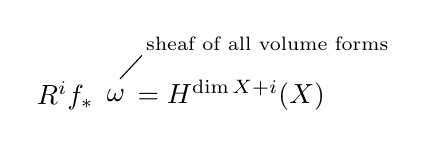
\begin{tikzpicture}[baseline=(omega.base)]
\node (omega) at (0,0) {$\omega$};
\node[anchor=east] at (-0.16,0) {$R^if_*$};
\node[anchor=west] at (0.15,0) {$=H^{\dim X+i}(X)$};
\node[anchor=west] at (0.26,0.66) {\scriptsize sheaf of all volume forms};
\draw (0.05,0.21) -- (0.33,0.51);
\end{tikzpicture}}\endgroup
\par (11)}
\end{GelfandAdjacentEvidence}
\begin{GelfandAdjacentEvidence}{GELFAND-P000941}{9}


More gen.: \uwave{For a smooth morphism, sheaves of cohom. along the fibers!}
\begin{equation*}
 \ldots\longrightarrow\mathcal M\otimes\Lambda^2T_{X/Y}
 \longrightarrow\mathcal M\otimes T_{X/Y}\longrightarrow\mathcal M
 \quad\leftarrow\quad(\text{this is }DR_{X/Y}\mathcal M)
 \tag{12}
\end{equation*}
\SourceFigure{GELFAND-P000941}{relative-de-rham}{The short arrow points left from the parenthetical note toward the complex.}
\end{GelfandAdjacentEvidence}


\Needspace{7\baselineskip}
\begin{GelfandAdjacentEvidence}{GELFAND-P000942}{1}
\SourcePage{GELFAND-P000942}{26}

Then
\begin{equation*}
 Rf_\bullet(DR_{X/Y}\mathcal M)=Rf_*(\mathcal M)
 \tag{13}
\end{equation*}

Thus in the direct image of [inserted above: rel.] DeRhama one introduces \underline{the action of diff. operators} (!)
\SourceFigure{GELFAND-P000942}{relative-dr-complex-word}{The line reads “DeRhama”. The abbreviation for “relative” is inserted above its start.}
\end{GelfandAdjacentEvidence}
\begin{GelfandAdjacentEvidence}{GELFAND-P000942}{2}


(this is not obvious, since in the orig. sheaf [crossed out: \sout{it} (?)] [inserted above: unresolved] is absent). This action is called
\Unclear{GELFAND-P000942}{overwritten-word-before-net}{The lower word before “absent” is heavily retraced and tentatively reads “it”. A short insertion above it is unresolved.}
\end{GelfandAdjacentEvidence}
\begin{GelfandAdjacentEvidence}{GELFAND-P000942}{3}


\uwave{the Gauss–Manin connection.}

\underline{2nd case}

$X\overset f\longrightarrow Y$\qquad\uwave{embedding.}
\begin{equation*}
 \begin{aligned}
 Rf_*(\mathcal M)&=Rf_\bullet
 \left(\mathcal M\mathbin{\underset{\mathcal D_X}{\overset L\otimes}}\mathcal D_{X\to Y}\right)\\
 &=f_\bullet
 \left(\mathcal M\mathbin{\underset{\mathcal D_X}{\overset L\otimes}}\mathcal D_{X\to Y}\right)=
 \end{aligned}
 \tag{14}
\end{equation*}
\SourceFigure{GELFAND-P000942}{embedding-equality}{At the end of the manuscript line (14) another equals sign follows the second expression.}
\end{GelfandAdjacentEvidence}
\begin{GelfandAdjacentEvidence}{GELFAND-P000942}{4}


(The functor $f_\bullet$ is exact in this case ---)

--- no cohom. arises along the fibers
\[
 =f_\bullet\left(\mathcal M\mathbin{\underset{\mathcal D_X}{\otimes}}\mathcal D_{X\to Y}\right)
\]
(since $\otimes$ is exact in this case)

$\omega\rightsquigarrow$ forms extended by $\delta$-fns. in the transv. direction.

\underline{Holonomic modules.}

$X$ --- a var., $\mathcal M$ --- a finitely generated
\(\overset{\mathcal D_X\text{-}}{\text{module}}\) [crossed out: unresolved]
\SourceFigure{GELFAND-P000942}{module-insertion}{$\mathcal D_X$- is inserted above “module”.}
\end{GelfandAdjacentEvidence}
\begin{GelfandAdjacentEvidence}{GELFAND-P000942}{5}

\Incomplete{GELFAND-P000942}{cancelled-module-end}{The writing after “module” is crossed out. It resembles $\mathcal M$, but the reading is unresolved.}
\end{GelfandAdjacentEvidence}
\begin{GelfandAdjacentEvidence}{GELFAND-P000942}{6}


It is called \uwave{holonomic}, if $\forall\,x\in X$,
\[
 \text{\uwave{the cohomology of}}\quad Li_x^*\mathcal M\quad
 \text{\uwave{is finite-dimensional}}
\]
(stalk of the module over the point)
\SourceFigure{GELFAND-P000942}{point-inclusion-diagram}{The arrow $i_x$ goes from $x$ to $X$. A heavy unresolved stroke precedes $x$.%
\par\smallskip
\begingroup\color{black}\GelfandFitDiagram{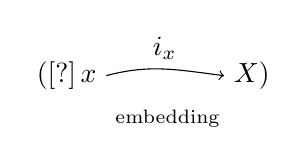
\begin{tikzpicture}[baseline=(x.base)]
\node (x) at (0,0) {$( [\text{?}]\,x$};
\node (X) at (2.35,0) {$X )$};
\draw[->] (x.east) to[out=15,in=173] node[above] {$i_x$} (X.west);
\node at (1.28,-0.55) {\scriptsize embedding};
\end{tikzpicture}}\endgroup}
\end{GelfandAdjacentEvidence}
\begin{GelfandAdjacentEvidence}{GELFAND-P000942}{7}


($i_x^*\mathcal M$ --- “freezing coeff.”, see above)

$\sim$ the complex $Li_x^*\mathcal M$ is finite-dimensional (since in the derived category).

\uwave{A free module}\quad\uwave{is not holonomic} (see last time)

Holonomicity $\sim$ overdeterminacy.

\underline{Examples}

a)\enspace [inserted above: $X=\mathbb R^1$ (?)] a bundle with an integr. connection
\SourceFigure{GELFAND-P000942}{example-a-field}{The field letter is retraced and has a slanting lower stroke. The tentative reading is $\mathbb R^1$.}
\end{GelfandAdjacentEvidence}
\begin{GelfandAdjacentEvidence}{GELFAND-P000942}{8}


The module is of this form except at a finite number of points where there may be sing.

b)\enspace $X=\mathbb C^2$ again on the complement of finitely many [crossed out: \sout{points} (?)]
[inserted above: curves] --- a bundle with an integr. conn.
\SourceFigure{GELFAND-P000942}{example-b-cancelled-word}{An earlier word is crossed out below the inserted “curves”. It may read “points”.}
\end{GelfandAdjacentEvidence}
\begin{GelfandAdjacentEvidence}{GELFAND-P000942}{9}


There are singularities on these curves.

\tikz[baseline=(q.base)]{\node[draw,circle,inner sep=2pt] (q) {?};}
\uwave{All are obtained by gluing} from modules obtained from $\delta$-fns. in the normal direction.
\SourceFigure{GELFAND-P000942}{circled-question}{A circled question mark stands to the left of the line about gluing.}
\end{GelfandAdjacentEvidence}
\begin{GelfandAdjacentEvidence}{GELFAND-P000942}{10}


[crossed out: \sout{(except for points […] curves} unresolved]
\Unclear{GELFAND-P000942}{last-cancelled-middle}{“Points” is tentatively read in the middle of the crossed-out line. The next word is unresolved.}
\end{GelfandAdjacentEvidence}
\begin{GelfandAdjacentEvidence}{GELFAND-P000942}{11}

\Incomplete{GELFAND-P000942}{last-cancelled-tail}{There is further crossed-out writing after “curves”. The ending is unresolved.}
\end{GelfandAdjacentEvidence}


\Needspace{7\baselineskip}
\begin{GelfandAdjacentEvidence}{GELFAND-P000943}{1}
\SourcePage{GELFAND-P000943}{unlabelled}

(15)\quad\underline{Thm.}\enspace 1) $\forall$ \uwave{holon. module has finite length}

(filtrations with irred. factors have the same length)
\Unclear{GELFAND-P000943}{filtration-length}{The ending of the first word in parentheses is indistinct. The last line reads “have the same length”.}
\end{GelfandAdjacentEvidence}
\begin{GelfandAdjacentEvidence}{GELFAND-P000943}{2}


2)\enspace \uwave{there is a descr. of all irreducibles}
\[
 Y\subset X,\qquad Y\text{ irred.}
\]

Irred. [inserted above and circled: flat] bundle $\mathcal L_Y$ with a connection on $Y$

(a vector bundle with an integr. conn.)
\SourceFigure{GELFAND-P000943}{flat-insertion}{A leader points from the circled “flat” to “bundle”.%
\par\smallskip
\begingroup\color{black}\GelfandFitDiagram{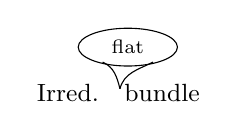
\begin{tikzpicture}[baseline=(b.base)]
\node (b) at (0,0) {\small Irred.\quad bundle};
\node (f) at (0.12,0.58) {\scriptsize flat};
\draw (f) ellipse (0.63 and 0.24);
\draw (-0.20,0.39) to[out=-24,in=104] (0.02,0.05);
\draw (0.02,0.05) to[out=76,in=-153] (0.44,0.39);
\end{tikzpicture}}\endgroup}
\end{GelfandAdjacentEvidence}
\begin{GelfandAdjacentEvidence}{GELFAND-P000943}{3}


2 pairs $Y_1,Y_2$ are called equiv. if $Y_1$ is open in $Y_2$

and
\[
 \mathcal L_{Y_1}=\left.\left(\mathcal L_{Y_2}\right)\right|_{Y_1}
\]
\SourceFigure{GELFAND-P000943}{generic-point}{The condition is written in the order “$Y_1$ is open in $Y_2$”.}
\end{GelfandAdjacentEvidence}
\begin{GelfandAdjacentEvidence}{GELFAND-P000943}{4}


(one can discard closed subsets, spec. over the generic point)

(16)\quad\underline{\underline{Assertion.}}\quad $i:Y\hookrightarrow X$

\uwave{In \(i_*\mathcal L_Y\) there is a unique irred. submodule} ---
\SourceFigure{GELFAND-P000943}{unique-submodule}{Two wavy underlines of different lengths appear below the line.}
\end{GelfandAdjacentEvidence}
\begin{GelfandAdjacentEvidence}{GELFAND-P000943}{5}


this is the object sought, an irred. module

$Y$ --- smooth $\Rightarrow$ already irreducible

At sing. there appear $\delta$-fns..
\SourceFigure{GELFAND-P000943}{terminal-vignette}{Below the last line are two tapered strokes with a dot between them.%
\par\smallskip
\begingroup\color{black}\GelfandFitDiagram{
\begin{tikzpicture}
\fill (-1.48,-0.05) -- (-0.31,0.14) -- (-0.31,-0.08) -- cycle;
\fill (0.02,-0.02) circle (0.11);
\fill (0.36,0.13) -- (1.54,0.05) -- (0.36,-0.08) -- cycle;
\end{tikzpicture}}\endgroup}
\end{GelfandAdjacentEvidence}


\Needspace{7\baselineskip}
\begin{GelfandAdjacentEvidence}{GELFAND-P000944}{1}
\SourcePage{GELFAND-P000944}{27}

$1/\underline{\overline{\mathrm{XII}}}$-80 \qquad \underline{Gelfand Sem.}
\SourceFigure{GELFAND-P000944}{hatched-date}{A narrow bar with transverse strokes underlines the date. Separate lines appear above and below XII.%
\par\smallskip
\begingroup\color{black}\GelfandFitDiagram{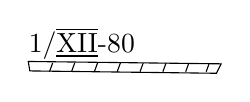
\begin{tikzpicture}[baseline=(date.base)]
\node[anchor=west,inner sep=0pt] (date) at (0,0) {$1/\underline{\overline{\mathrm{XII}}}$-80 };
\draw (0,-0.23) -- (2.45,-0.26) -- (2.39,-0.38) -- (0.02,-0.35) -- cycle;
\foreach \x in {0.31,0.59,0.88,1.17,1.46,1.75,2.04,2.30}
 {\draw (\x,-0.25) -- ++(-0.04,-0.11);}
\end{tikzpicture}}\endgroup}
\end{GelfandAdjacentEvidence}
\begin{GelfandAdjacentEvidence}{GELFAND-P000944}{2}


\underline{S. P. Novikov.}

\begin{equation*}
 \hat H=\frac12\sum_{\alpha=1}^n
 \left(i\frac{\partial}{\partial x^\alpha}-eA_\alpha\right)^2
 +cV(\vec x)
 \tag{1}
\end{equation*}
\Incomplete{GELFAND-P000944}{equation-one-cancellation}{Heavily crossed-out writing appears after the equals sign in (1), before the fraction. Its reading is unresolved.}
\end{GelfandAdjacentEvidence}
\begin{GelfandAdjacentEvidence}{GELFAND-P000944}{3}


\begin{equation*}
 H_{\alpha\beta}=\partial_\beta A_\alpha-\partial_\alpha A_\beta
 \tag{2}
\end{equation*}
$V$ --- el. field, $H_{\alpha\beta}$ --- magn. field

\begin{equation*}
 \hat H\psi=\varepsilon\psi\qquad\text{spectr. problem.}
 \tag{3}
\end{equation*}

The interesting case is when

(4)\quad $H_{\alpha\beta}(x)$ and $V(x)$ are periodic with a lattice of periods.
\SourceFigure{GELFAND-P000944}{lattice-cell}{Cell $K_{12}$ lies between the arrows $T_1,T_2$. The top and right sides are broken lines.%
\par\smallskip
\begingroup\color{black}\GelfandFitDiagram{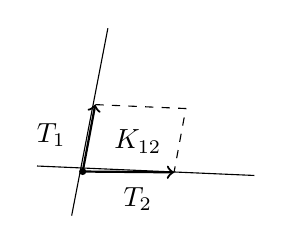
\begin{tikzpicture}
\draw (-0.58,0.07) -- (2.18,-0.05);
\draw (-0.14,-0.56) -- (0.32,1.82);
\draw[thick,->] (0,0) -- (0.16,0.85);
\draw[thick,->] (0,0) -- (1.16,-0.01);
\draw[dashed] (0.16,0.85) -- (1.31,0.80) -- (1.16,-0.01);
\fill (0,0) circle (0.045);
\node at (-0.40,0.46) {$T_1$};
\node at (0.70,-0.35) {$T_2$};
\node at (0.70,0.38) {$K_{12}$};
\end{tikzpicture}}\endgroup}
\end{GelfandAdjacentEvidence}
\begin{GelfandAdjacentEvidence}{GELFAND-P000944}{4}


(not only the el. field but also its potential. A constant el. field --- unreasonable)
\Unclear{GELFAND-P000944}{constant-electric-word}{The word after the dash is tentatively read as «неразумно» (“unreasonable”). Its ending is faint.}
\end{GelfandAdjacentEvidence}
\begin{GelfandAdjacentEvidence}{GELFAND-P000944}{5}


--- the potential then $\vec E\cdot\vec x$ [crossed out: unresolved] ---
\Incomplete{GELFAND-P000944}{electric-potential-cancellation}{One sign is crossed out after $\vec E\cdot\vec x$. The exact reading is unresolved.}
\end{GelfandAdjacentEvidence}
\begin{GelfandAdjacentEvidence}{GELFAND-P000944}{6}


\uwave{--- even the 1-dim. problem is unstudied.})

$A_\alpha$ is nonperiodic (generally speaking).

$K_{\alpha\beta}$ --- an elem. cell, spanned by the $\alpha$ and $\beta$ coordinate
\Unclear{GELFAND-P000944}{cell-preposition}{The overwritten preposition after “spanned” is tentatively read as «на».}
\end{GelfandAdjacentEvidence}
\begin{GelfandAdjacentEvidence}{GELFAND-P000944}{7}

\Unclear{GELFAND-P000944}{cell-coordinate-ending}{The end of the word for “coordinate” is overwritten. The last letter reads «у».}
\end{GelfandAdjacentEvidence}
\begin{GelfandAdjacentEvidence}{GELFAND-P000944}{8}


\begin{equation*}
 \iint_{K_{\alpha\beta}}H_{\alpha\beta}\,dx^\alpha\wedge dx^\beta
 =\Phi_{\alpha\beta}\qquad\text{--- magn. fluxes (basis)}
 \tag{5}
\end{equation*}
(no summation!)

\begin{equation*}
 i\nabla_\alpha=i\frac{\partial}{\partial x^\alpha}-eA_\alpha
 \qquad\text{has the meaning of a connection}
 \tag{6}
\end{equation*}

\underline{Rem.} The spin here is $0$, with spin $1/2$ one has
\begin{equation*}
 \hat H=(1)+e\sigma_jH^j,\qquad\text{where }
 H^1=H_{23},\quad H^2=-H_{13},\quad H^3=H_{12};
 \tag{7}
\end{equation*}
$\sigma_1,\sigma_2,\sigma_3$ --- Pauli matr.

(8)\quad\uwave{Admissible case:} \(\dfrac e{2\pi}\Phi_{\alpha\beta}\in\mathbb Z\)

The operator $\hat H$ is consid. in $L^2(\mathbb R^n)$.

(9)\quad $(8)\Rightarrow\hat H$ --- a univ. cover. op. on the torus (in a bundle), moreover
\Unclear{GELFAND-P000944}{covering-overwritten-word}{The beginning of the word for “moreover” is retraced.}
\end{GelfandAdjacentEvidence}
\begin{GelfandAdjacentEvidence}{GELFAND-P000944}{9}


\begin{equation*}
 \left(c_1(\xi),\underset{\substack{\vert\\\text{basis cycle}}}{Z_{\alpha\beta}}\right)
 =\frac e{2\pi}\Phi_{\alpha\beta}
 \tag{10}
\end{equation*}
\SourceFigure{GELFAND-P000944}{chern-cycle}{A short stroke below $Z_{\alpha\beta}$ leads to “basis cycle”.}
\end{GelfandAdjacentEvidence}
\begin{GelfandAdjacentEvidence}{GELFAND-P000944}{10}


But the op. always makes sense (phys.), yet there is no theory.

(11)\quad Irrational is of int. \uwave{Ration. reduces to it by coarsening the lattice}
\Unclear{GELFAND-P000944}{irrational-final-abbreviation}{The abbreviation after “Irrational” is tentatively read as «интер.» (“of int.”).}
\end{GelfandAdjacentEvidence}


\Needspace{7\baselineskip}
\begin{GelfandAdjacentEvidence}{GELFAND-P000945}{1}
\SourcePage{GELFAND-P000945}{unlabelled}

\dashuline{Magnetic translations.}
\SourceFigure{GELFAND-P000945}{broken-underline}{A broken line underlines the heading.}
\end{GelfandAdjacentEvidence}
\begin{GelfandAdjacentEvidence}{GELFAND-P000945}{2}


\underline{2 types of problems:} a) [crossed out: \sout{magn.} (?)] the lattice is imposed (solid state!), and the magn. field is external
\Unclear{GELFAND-P000945}{top-cancelled-abbreviation}{The crossed-out abbreviation before “lattice” is tentatively read as “magn.”.}
\end{GelfandAdjacentEvidence}
\begin{GelfandAdjacentEvidence}{GELFAND-P000945}{3}


b)\enspace of superconduct. type: the magn. field arises on its own, they are automatically integral.

a)\enspace $K_{\alpha\beta}\sim10^{-10}\text{ cm}^2$
\qquad b)\enspace $\sim10^{-16}\text{ cm}^2$
\SourceFigure{GELFAND-P000945}{cell-areas}{The line reads $10^{-10}$ and $10^{-16}$ in square centimeters.}
\end{GelfandAdjacentEvidence}
\begin{GelfandAdjacentEvidence}{GELFAND-P000945}{4}


\underline{Magn. transl.}\qquad We have:
\begin{equation*}
 A_\alpha(\ldots,x^i+T_i,\ldots)=A_\alpha(x)+\partial_\alpha f_i
 \tag{12}
\end{equation*}
(since $dA$ is periodic)

\begin{equation*}
 \hat T_j^*\psi(x)=\psi(\mathinner{..}\,x^{j}+T_j,\,)\exp(-ie f_j)
 \tag{13}
\end{equation*}
(operator of magn. translation)
\Unclear{GELFAND-P000945}{translation-coordinate-superscript}{In (13) the superscript of $x$ is retraced. The reading $j$ is tentative and agrees with $T_j$ on the same line.}
\end{GelfandAdjacentEvidence}
\begin{GelfandAdjacentEvidence}{GELFAND-P000945}{5}


(14)\quad\underline{Lemma 1} (known $\sim$1960s
[crossed out: unresolved], \uwave{Zak and Brown})
\begin{equation*}
 \hat T_j^*\hat T_k^*=\hat T_k^*T_j^*\exp(-ie\Phi_{kj}),
 \qquad j,k=1,\ldots,n.
\end{equation*}
\Unclear{GELFAND-P000945}{lemma-cancelled-character}{A sign after “1960s” is heavily retraced. Its exact reading is unresolved.}
\end{GelfandAdjacentEvidence}
\begin{GelfandAdjacentEvidence}{GELFAND-P000945}{6}

\SourceFigure{GELFAND-P000945}{commutator-hats}{The last $T_j^*$ on the right side of the equality has no visible hat.}
\end{GelfandAdjacentEvidence}
\begin{GelfandAdjacentEvidence}{GELFAND-P000945}{7}


This gives a projective repr. of an ab. group, with cocycles specified in advance.

Irrat. fluxes $\Rightarrow$ one gets groups not of type 1. (subgr. of the Heisenberg grp.).

\begin{equation*}
 \frac{e\Phi_{kj}}{2\pi}\in\mathbb Z\Rightarrow\text{commut. group}
 \tag{15}
\end{equation*}
$\underline{n=2}$

($n=3$ is also interesting)

superconduct. is a 2-dim. problem

\underline{Problem:} describe the spectrum of $\hat H$.

(16)\quad $[\hat H,\hat T_j^*]=0\Rightarrow$ the eigenfns. must be sought as simultaneous eigenfns. for $\hat T_j^*$

[crossed out below the line: \sout{magn.} (?)]
\Unclear{GELFAND-P000945}{eigenfunction-cancelled-abbreviation}{Below line (16) the crossed-out abbreviation resembles “magn.”.}
\end{GelfandAdjacentEvidence}
\begin{GelfandAdjacentEvidence}{GELFAND-P000945}{8}


Magnetic Bloch:
\begin{equation*}
 \hat T_j^*\psi_{p}=\exp(ip_jT_j)\psi_{p}
 \tag{17}
\end{equation*}
\Unclear{GELFAND-P000945}{bloch-subscript-left}{The left $\psi$ subscript is heavily retraced. $p$ is tentatively supplied from the neighboring line.}
\end{GelfandAdjacentEvidence}
\begin{GelfandAdjacentEvidence}{GELFAND-P000945}{9}

\Unclear{GELFAND-P000945}{bloch-subscript-right}{The right $\psi$ subscript is also heavily retraced. $p$ is tentatively supplied.}
\end{GelfandAdjacentEvidence}
\begin{GelfandAdjacentEvidence}{GELFAND-P000945}{10}


Op. in $L^2$ $=$ direct integral of op. on the torus with such bound. conds.

$p_j$ --- \uwave{quasimomenta}\qquad $(p_1,p_2)\in\mathbb T^2$
\qquad (torus of the recip. lattice)

Fix $p_1,p_2\Rightarrow$ an op. in a bundle on the torus with eigenvals.
\SourceFigure{GELFAND-P000945}{fixed-eigenvalues}{The last two abbreviations read “eigenvals.”.}
\end{GelfandAdjacentEvidence}


\begin{equation*}
 \varepsilon_j(p_1,p_2)\qquad\text{--- dispersion law}
 \tag{18}
\end{equation*}
\[
 j=1,2,\ldots
\]

\Needspace{7\baselineskip}
\begin{GelfandAdjacentEvidence}{GELFAND-P000946}{1}
\SourcePage{GELFAND-P000946}{28}

(19) \underline{Theorem}. \underline{Let} $V=0$, \underline{spin} $s=\frac12$,
\[
 n=2,\qquad N\underset{\mathrm{def}}{=}\frac{e\Phi_{12}}{2\pi}.
\]

[In the right margin, beyond the double line]\par
Dubrovin, Novikov\par
ZhETF, Sept. 1980.\par
and there is also a paper in DAN
\SourceFigure{GELFAND-P000946}{marginal-citation}{References in the right margin.}
\end{GelfandAdjacentEvidence}
\begin{GelfandAdjacentEvidence}{GELFAND-P000946}{2}


(magn. field directed along the $Z$ axis --- 2-dim. case --- and periodic)

\underline{Then} \underline{given} $A=(a_1,\ldots,a_N)\in C^N$, \underline{we} \underline{get} \underline{that} the \underline{eigen}fn. \underline{has the form}
[inserted above “eigen” $(\forall\ \text{magn.-Bloch})$]
\SourceFigure{GELFAND-P000946}{bloch-insertion}{A curved stroke links the insertion above the line to the main text.}
\end{GelfandAdjacentEvidence}
\begin{GelfandAdjacentEvidence}{GELFAND-P000946}{3}


\begin{equation*}
 \Psi_A=\exp(-e\varphi)\prod_{j=1}^N\sigma(z-a_j)\exp(-az).
 \tag{20}
\end{equation*}
\SourceFigure{GELFAND-P000946}{sigma-exp-sign}{The sign before $az$ in (20) is minus.}
\end{GelfandAdjacentEvidence}
\begin{GelfandAdjacentEvidence}{GELFAND-P000946}{4}

($\sigma$ --- Weierstrass elliptic fn.)\par
one of the $\theta$-fns.
\SourceFigure{GELFAND-P000946}{sigma-note}{Note at the right of (20).}
\end{GelfandAdjacentEvidence}
\begin{GelfandAdjacentEvidence}{GELFAND-P000946}{5}


\begin{equation*}
 p=p_1+ip_2=\frac{2\pi i}{T_1T_2}\sum a_j+
 \underset{\substack{\vert\\\text{depends on the magn. field}}}{\operatorname{const}(H)},
 \tag{21}
\end{equation*}
\SourceFigure{GELFAND-P000946}{quasimomentum-sign}{The summation term in (21) has a plus sign.}
\end{GelfandAdjacentEvidence}
\begin{GelfandAdjacentEvidence}{GELFAND-P000946}{6}

\SourceFigure{GELFAND-P000946}{field-constant}{A line connects the annotation below $\operatorname{const}(H)$ to that term.}
\end{GelfandAdjacentEvidence}
\begin{GelfandAdjacentEvidence}{GELFAND-P000946}{7}

\[
 \mathcal D=\sum a_j.\qquad\text{(divisor)}
\]

(22) [crossed out: \sout{\(\varphi(x,y)\)} (?)]
\begin{equation*}
 \varphi(x,y)=\frac{1}{2\pi}\int_{K_{12}}\ln|\sigma(z-z')|H(z')\,d^2z'.
\end{equation*}
\Unclear{GELFAND-P000946}{eq22-cancel}{The crossed-out entry before (22) is tentatively read as $\varphi(x,y)$.}
\end{GelfandAdjacentEvidence}
\begin{GelfandAdjacentEvidence}{GELFAND-P000946}{8}

\(z={}\)[crossed out: entry unresolved] \(x+iy\).
\Incomplete{GELFAND-P000946}{z-cancel}{Several signs are crossed out after the equals sign. Their exact reading is unresolved.}
\end{GelfandAdjacentEvidence}
\begin{GelfandAdjacentEvidence}{GELFAND-P000946}{9}


Fns. (20) --- a complete basis of solutions to the eq. $\hat H\psi=0$

(exact integr. at the lower zero energy level)
\SourceFigure{GELFAND-P000946}{exact-abbr}{The abbreviation after “exact” reads “integr.”}
\end{GelfandAdjacentEvidence}
\begin{GelfandAdjacentEvidence}{GELFAND-P000946}{10}


[crossed out: $L^2=(L^2)^0+\ldots$ (?)]
\Incomplete{GELFAND-P000946}{l2-cancel}{The beginning of the crossed-out formula is a tentative reading. The end after the plus sign is unresolved.}
\end{GelfandAdjacentEvidence}
\begin{GelfandAdjacentEvidence}{GELFAND-P000946}{11}

\[
 L_2=L_2+L_2^\perp.
\]
\SourceFigure{GELFAND-P000946}{l2-split}{The loop above the first $L_2$ on the right continues into a descender from the line above.}
\end{GelfandAdjacentEvidence}
\begin{GelfandAdjacentEvidence}{GELFAND-P000946}{12}


\begin{equation*}
 a=a(a_1,\ldots,a_N)\quad\text{--- \underline{is calculated}}.
 \tag{23}
\end{equation*}

Selecting the dependence (23) --- is selecting real \underline{quasimomenta}

(the fn. $\Psi_A$ is always an eigenfn. and Bloch).

$\lambda\Psi_A$ is also an eigenfn.

$(\lambda,a_1,\ldots,a_N)$ --- the full set of parameters.

\underline{Rem.}
\begin{equation*}
 (\lambda,a_1,\ldots,a_N)\overset{P}{\longrightarrow}\mathbb T^2.
 \tag{24}
\end{equation*}

(25) We get [crossed out: entry unresolved] \underline{a holom. vect. bundle}
($N$-dimensional) over $\mathbb T^2$ with $\underline{c_1=N}$.
\Incomplete{GELFAND-P000946}{eq25-cancel}{The heavily crossed-out entry before “holom.” is unresolved.}
\end{GelfandAdjacentEvidence}
\begin{GelfandAdjacentEvidence}{GELFAND-P000946}{13}


(= the number of quanta of magn. flux)

(26) \underline{Fibre} --- at fixed $p$ --- We get
$\underline{\underline{\mathcal L(\mathcal D)}}$,
$\dim\mathcal L(\mathcal D)=N$

[crossed out: \sout{Next} (?)] (mult. by a doubly periodic fn.)
\Unclear{GELFAND-P000946}{eq26-cancel}{The crossed-out entry is tentatively read as “Next”.}
\end{GelfandAdjacentEvidence}
\begin{GelfandAdjacentEvidence}{GELFAND-P000946}{14}


$\mathcal D$ --- the divisor of zeros of $\sigma$\par
$\mathcal D=\sum a_j$\par
(divisor)
\SourceFigure{GELFAND-P000946}{divisor-margin}{The note on the divisor in the right margin.}
\end{GelfandAdjacentEvidence}


In fact (26) --- from the Atiyah–Singer thm.
\[
 (\operatorname{Coker}=0)
\]
infinite-dimensional machinery.

\underline{Magn. field here:}
\begin{equation*}
 A_1=-\partial_2\varphi,\quad A_2=\partial_1\varphi,\quad\Delta\varphi=H.
 \tag{27}
\end{equation*}

$a_1,\ldots,a_N$ are determ. mod the lattice and symmetrized, i.e.
\[
 a\in S^N\Gamma.
\]

\Needspace{7\baselineskip}
\begin{GelfandAdjacentEvidence}{GELFAND-P000947}{1}
\SourcePage{GELFAND-P000947}{unlabelled}

The fibre (25) is a lin. space. (not immediately obvious)

All fns. $\Psi_A$ in a fixed fibre are obt. from one by mult. by ellipt. (?) 2-periodic fns..
\Unclear{GELFAND-P000947}{top-elliptic}{The abbreviation is tentatively read as the Russian “эллипт.”; “эллип.” is also possible.}
\end{GelfandAdjacentEvidence}
\begin{GelfandAdjacentEvidence}{GELFAND-P000947}{2}


\underline{Corollary:} Bloch fns. form, form a linear bundle.

\uwave{Eigenfns. at fixed} $p$ \uwave{form an} $N$-\uwave{dimensional space (!)}

(\dashuline{the dimension is fixed})

In a uniform magn. field the \dashuline{assert. holds} for all energy levels.

[crossed out: \underline{\sout{Question 2.}} \sout{Where does the degeneracy come from?}]
\SourceFigure{GELFAND-P000947}{crossed-question}{The whole question is crossed out.}
\end{GelfandAdjacentEvidence}
\begin{GelfandAdjacentEvidence}{GELFAND-P000947}{3}


Now let us perturb:
\begin{equation*}
 \hat H=\hat H_0+e\,v(x,y)\qquad\text{(with the same grp. of periods).}
 \tag{28}
\end{equation*}

(29) \underline{Theorem 2}. \dashuline{Perturb. op.} --- \dashuline{quadr. form of general type}.

(2-param. family of quadr. forms in general pos. among all complex Hermitian forms).

I.e. if one excludes the set of potentials on whose Fourier coeffs. 3 eqs. are imposed, then the spectrum (Bloch eigenfns.) has the following properties
\begin{equation*}
 \hat V_{(p_1,p_2)}(\Psi_A)=\iint_{K_{12}}\bar\Psi_A\,v\Psi_A\,dx\,dy.
 \tag{30}
\end{equation*}

(complex Hermitian form, $\Psi_A$ --- eigenfns. of $H_0$)

at fixed quasimomenta.

(30) Is in general position (as an operator)

Quadr. form in general pos. --- no pair of eigen [crossed out: \sout{fns.} (?)] values coalesces
\Unclear{GELFAND-P000947}{eigen-cancel}{The crossed-out entry before “values” is tentatively read as “fns.”}
\end{GelfandAdjacentEvidence}
\begin{GelfandAdjacentEvidence}{GELFAND-P000947}{4}


The map of the torus into the set of quadr. forms is \uwave{in general position}.

(In the 1-dim. case --- it is never in general position)

because the op. is of 2nd order.

([crossed out: $\Rightarrow$ (?); inserted below: since] codim. 3,
[crossed out: \sout{then} (?)] then it does not intersect with mult. eigenvals.,
\Unclear{GELFAND-P000947}{codim-firstmark}{The crossed-out sign is tentatively read as $\Rightarrow$.}
\end{GelfandAdjacentEvidence}
\begin{GelfandAdjacentEvidence}{GELFAND-P000947}{5}

\Unclear{GELFAND-P000947}{codim-cancel-top}{The heavily crossed-out entry before “then” is tentatively read as “then”.}
\end{GelfandAdjacentEvidence}
\begin{GelfandAdjacentEvidence}{GELFAND-P000947}{6}


$\underline{\underline{n=3}}$ [crossed out: \sout{codim. 2} (?)] $\Rightarrow$
[crossed out: initial Cyrillic “в” (?); the rest is unresolved] it inters. at isolated points.)
\Unclear{GELFAND-P000947}{codim-cancel-left}{The crossed-out text is tentatively read as “codim. 2”.}
\end{GelfandAdjacentEvidence}
\begin{GelfandAdjacentEvidence}{GELFAND-P000947}{7}

\Incomplete{GELFAND-P000947}{codim-cancel-right}{After the arrow, the initial stroke resembles Cyrillic “в”. The cancellation obscures the rest.}
\end{GelfandAdjacentEvidence}
\begin{GelfandAdjacentEvidence}{GELFAND-P000947}{8}

\SourceFigure{GELFAND-P000947}{codimension-lines}{The two codimension lines, with “since” inserted below the first cancellation.}
\end{GelfandAdjacentEvidence}


\underline{\underline{Corollary:}}

$\underline{n=2}\quad\Rightarrow$ the bundle splits into 1-dimensional ones

\underline{\underline{I.M.G.:}}

The irrat. case is interesting!

(there everything is in fact noncommutative)

Idea: go into the complex domain (inside the circle!) --- in a non-self-adjoint situation

i.e. carry out a \uwave{regularization} (parabolic)

\Needspace{7\baselineskip}
\begin{GelfandAdjacentEvidence}{GELFAND-P000948}{1}
\SourcePage{GELFAND-P000948}{29}

\underline{Irrat. case:}
\[
 H_{12}=\frac{\partial A_1}{\partial x_2}-\frac{\partial A_2}{\partial x_1},
 \qquad A_1\,dx_1+A_2\,dx_2.
\]
\SourceFigure{GELFAND-P000948}{curvature-order}{The order of derivatives in $H_{12}$ follows the manuscript.}
\end{GelfandAdjacentEvidence}
\begin{GelfandAdjacentEvidence}{GELFAND-P000948}{2}

\[
 \left[\left(i\frac{\partial}{\partial x_1}-A_1\right)^2+
 \left(i\frac{\partial}{\partial x_2}-A_2\right)^2\right]=\hat H.
\]
\[
 H_{12}(x_1+m_1T_1,x_2+m_2T_2)=H_{12}(x_1,x_2)
\]
\[
 \Phi_{12}=\iint H_{12}\,dx_1\wedge dx_2.
\]
\[
 \Phi_{12}\ne2\pi\frac{N}{M}
\]

\uwave{Group:}
\[
 \hat T_1^*\hat T_2^*=\hat T_2^*\hat T_1^*\exp(-i\Phi_{12})
\]
acts on the set of all fns. (fixed eigen [crossed-out entry unresolved] subspace)
\Incomplete{GELFAND-P000948}{subspace-cancel}{Dense hatching obscures the entry between “eigen” and “subspace”.}
\end{GelfandAdjacentEvidence}
\begin{GelfandAdjacentEvidence}{GELFAND-P000948}{3}


$[H,\hat T_j^*]=0$ still (choice of $f_j$ in (12)--(13)).

At the basis of the theory [inserted above the line: of factors] of von Neumann --- \uwave{irreducibility ergodicity}.
\SourceFigure{GELFAND-P000948}{factors-insertion}{A curved mark connects “of factors” above the line with the position after “theory”.}
\end{GelfandAdjacentEvidence}
\begin{GelfandAdjacentEvidence}{GELFAND-P000948}{4}

\SourceFigure{GELFAND-P000948}{ergodicity-line}{One wavy line underlines both words.}
\end{GelfandAdjacentEvidence}
\begin{GelfandAdjacentEvidence}{GELFAND-P000948}{5}


\underline{I.M.G.} To know by next semester: $G$-structures, $\mathcal D$-structures and the Spencer resolution.
\SourceFigure{GELFAND-P000948}{structures-letter}{The two structures are denoted by $G$ and a calligraphic $\mathcal D$.}
\end{GelfandAdjacentEvidence}


\Needspace{7\baselineskip}
\begin{GelfandAdjacentEvidence}{GELFAND-P000949}{1}
\SourcePage{GELFAND-P000949}{51}

\underline{\underline{9/II-81}}.\qquad \underline{Gelfand seminar.}

\underline{MacPherson}.
\SourceFigure{GELFAND-P000949}{macpherson-name}{The manuscript gives the name in Latin script.}
\end{GelfandAdjacentEvidence}
\begin{GelfandAdjacentEvidence}{GELFAND-P000949}{2}


(\uwave{On joint work with I. M. Gelfand.})

Problem --- find interesting polyhedra in Grassmannians.

In proj. spaces polyhedra have \uwave{flat} faces
(face $\subset$ subspace of smaller dim.)
\begin{equation*}
 P_1\subset P_2\subset P_3\subset\ldots
 \tag{0}
\end{equation*}
(projective)

$G_n^m$ --- $n$-planes in $\mathbb R^{m+n}$ (subspaces)

Embeddings:
\begin{equation*}
 \begin{array}{ccccccc}
 G_1^1 & \subset & G_1^2 & \subset & G_1^3 & \subset & \ldots\\
 \cap  &         & \cap  &         & \cap  &         & \\
 G_2^1 & \subset & G_2^2 & \subset & G_1^3 & \subset & \ldots
 \end{array}
 \tag{1}
\end{equation*}
\SourceFigure{GELFAND-P000949}{embeddings-lower-index}{The third entry in the lower row reads $G_1^3$.}
\end{GelfandAdjacentEvidence}
\begin{GelfandAdjacentEvidence}{GELFAND-P000949}{3}

and so on

We want: faces --- polyh. in smaller ones

Picture (0) corresp. to the upper row of (1).

Naïve method:
\SourceFigure{GELFAND-P000949}{geodesic-triangle}{Triangle with wavy sides and a fan of strokes. The broken interior strokes are drawn approximately.
\par\smallskip
\begingroup\color{black}\GelfandFitDiagram{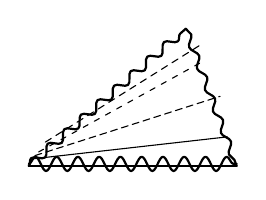
\begin{tikzpicture}[x=0.66cm,y=0.66cm,line cap=round,line join=round]
  \draw[thick] (0,0)--(4,0);
  \draw[thick,decorate,decoration={snake,amplitude=0.055cm,segment length=0.28cm}]
    (0,0)--(3.02,2.64);
  \draw[thick,decorate,decoration={snake,amplitude=0.041cm,segment length=0.29cm}]
    (3.02,2.64)--(4,0);
  \draw[thick,decorate,decoration={snake,amplitude=0.09cm,segment length=0.27cm}]
    (0,0.04)--(4,0.04);
  \draw (0.1,0.14)--(3.82,0.56);
  \draw[dash pattern=on 2.5pt off 1.6pt] (0.12,0.2)--(3.68,1.34);
  \draw[dash pattern=on 2pt off 2.6pt] (0.19,0.27)--(3.4,2.04);
  \draw[dash pattern=on 2.5pt off 2pt] (0.32,0.46)--(3.32,2.34);
\end{tikzpicture}}\endgroup
}
\end{GelfandAdjacentEvidence}
\begin{GelfandAdjacentEvidence}{GELFAND-P000949}{4}

there is a triangle of 3 geod.

How to fill it in?

also with geod. (segments)

If one does this in the Grassmannian, it does not work.

Here one gets
\[
 \mathrm{Rank}\geqslant 2
\]
\SourceFigure{GELFAND-P000949}{rank-sign}{The sign between “Rank” and $2$ reads $\geqslant$.}
\end{GelfandAdjacentEvidence}
\begin{GelfandAdjacentEvidence}{GELFAND-P000949}{5}


(2) \underline{Defin.}\par
\underline{Hypersimplex $\Delta_n^m$}: set of points
\[
 (x_1,\ldots,x_{n+m})\in\mathbb R^{n+m},
\]
satisfying the rels.
\begin{gather*}
 0\leq x_i\leq 1,\\
 \sum_i x_i=n
\end{gather*}
[crossed out after $n$: \sout{\mbox{\(+1\)}} (?)]
\Unclear{GELFAND-P000949}{hypersimplex-cancellation}{Hatching obscures the entry after $n$. The reading $+1$ is tentative; the letter $m$ is also possible.}
\end{GelfandAdjacentEvidence}
\begin{GelfandAdjacentEvidence}{GELFAND-P000949}{6}


(3) \underline{Def.}\qquad \uwave{Grassm. complex} in $P_{n+m-1}$:
choose $n+m$ points $e_1,\ldots,e_{n+m}$, not lying in a hypersubspace of smaller dim. (a hyperplane).

$H^0$ = conn. comp. of $1$ of the subgroup of $PGL(n+m)$, which leaves these points fixed.
\SourceFigure{GELFAND-P000949}{identity-component}{The digit $1$ follows the abbreviation for component.}
\end{GelfandAdjacentEvidence}
\begin{GelfandAdjacentEvidence}{GELFAND-P000949}{7}


Grasm. complex --- closure of an orbit in \uwave{gen. pos.} of the group $H^0$,
acting on $G_n^m$.
[written beneath “gen. pos.” \textit{generic}.]
\SourceFigure{GELFAND-P000949}{generic-gloss}{The English gloss appears below the wavy underline.}
\end{GelfandAdjacentEvidence}


(4) \underline{\textit{generic} --- ?}

this means $H^0\xi$

$\xi$ --- subspace transverse to all coord. subspaces:

if $e_1,\ldots,e_{n+m}$ are taken as a basis (some points on them)

this is not the same as $\dim=\max$ (!)

\Needspace{7\baselineskip}
\begin{GelfandAdjacentEvidence}{GELFAND-P000950}{1}
\SourcePage{GELFAND-P000950}{unlabelled}

(5) \underline{Theorem}. \uwave{These 2 objects are diffeomorphic.}

def. (3) can be given for $\forall$ semisimple group.
\SourceFigure{GELFAND-P000950}{definition-verb}{The abbreviated verb before “for” reads “прив.”.}
\end{GelfandAdjacentEvidence}
\begin{GelfandAdjacentEvidence}{GELFAND-P000950}{2}


$G_n^m$ --- $(n-1)$-subspaces in $P_{n+m-1}$ (?).
\Unclear{GELFAND-P000950}{projective-index}{The first character of the index is heavily retraced. The reading $P_{n+m-1}$ is tentative; $P_{m+n-1}$ is also possible.}
\end{GelfandAdjacentEvidence}
\begin{GelfandAdjacentEvidence}{GELFAND-P000950}{3}


(6) \underline{Example}. \quad $\Delta_1^2\qquad G_1^2$

\SourceFigure{GELFAND-P000950}{cube-section}{Cube with hatched section $H$. The interior label, tentatively $x_3$, is overlapped by lines.
\par\smallskip
\begingroup\color{black}\GelfandFitDiagram{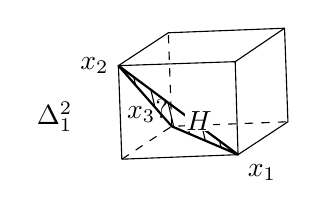
\begin{tikzpicture}[x=0.72cm,y=0.72cm,line join=round]
  \coordinate (o) at (0,0);
  \coordinate (x) at (2.05,0.08);
  \coordinate (y) at (-0.06,1.65);
  \coordinate (z) at (0.88,0.58);
  \coordinate (xy) at (2,1.72);
  \coordinate (xz) at (2.93,0.66);
  \coordinate (yz) at (0.82,2.23);
  \coordinate (xyz) at (2.87,2.31);
  \draw (o)--(x)--(xy)--(y)--cycle;
  \draw (y)--(yz)--(xyz)--(xy) (xyz)--(xz)--(x);
  \draw[dashed] (o)--(z)--(xz) (z)--(yz);
  \begin{scope}
    \clip (x)--(y)--(z)--cycle;
    \foreach \a in {0.3,0.55,...,1.8}{\draw[thin] (\a,0)--++(-0.4,1.7);}
  \end{scope}
  \draw[thick] (x)--(y)--(z)--cycle;
  \node[left] at (-0.7,0.75) {$\Delta_1^2$};
  \node[left] at (y) {$x_2$};
  \node[below right] at (x) {$x_1$};
  \node[above left,inner sep=1pt] at (z) {$x_3?$};
  \node[fill=white,inner sep=0.5pt] at (1.36,0.68) {$H$};
\end{tikzpicture}}\endgroup
}
\end{GelfandAdjacentEvidence}
\begin{GelfandAdjacentEvidence}{GELFAND-P000950}{4}


\SourceFigure{GELFAND-P000950}{projective-triangle}{Three lines through the marked points $e_1,e_2,e_3$. The Roman numerals and hatching follow the manuscript.
\par\smallskip
\begingroup\color{black}\GelfandFitDiagram{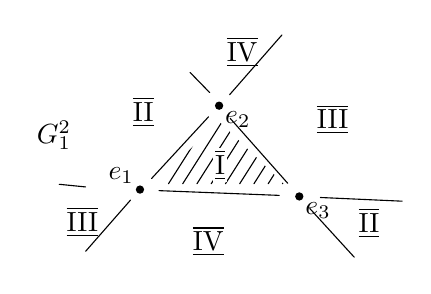
\begin{tikzpicture}[x=0.67cm,y=0.67cm,line cap=round]
  \coordinate (a) at (-1.42,-0.01);
  \coordinate (b) at (0.08,1.58);
  \coordinate (c) at (1.6,-0.14);
  \draw (-2.45,-1.18)--(-1.6,-0.21) (-1.2,0.2)--(-0.12,1.37) (0.28,1.79)--(1.27,2.92);
  \draw (-0.47,2.21)--(-0.1,1.83) (0.29,1.34)--(1.38,0.11) (1.8,-0.37)--(2.64,-1.29);
  \draw (-2.95,0.09)--(-2.45,0.04) (-1.06,-0.03)--(1.22,-0.12) (2,-0.16)--(3.55,-0.23);
  \begin{scope}
    \clip (-1.16,0.04)--(0.06,1.3)--(1.4,0.01)--cycle;
    \foreach \a in {-1.15,-0.88,...,1.3}{\draw[thin] (\a,0.1)--++(0.87,1.37);}
  \end{scope}
  \foreach \point in {a,b,c}{\fill (\point) circle[radius=1.5pt];}
  \node[above left,inner sep=2pt] at (a) {$e_1$};
  \node[below right,inner sep=2pt] at (b) {$e_2$};
  \node[below right,inner sep=2pt] at (c) {$e_3$};
  \node at (-3.05,1.02) {$G_1^2$};
  \node[fill=white,inner sep=0.7pt] at (0.1,0.46) {$\overline{\underline{\mathrm{I}}}$};
  \node at (-1.36,1.46) {$\overline{\underline{\mathrm{II}}}$};
  \node at (2.23,1.32) {$\overline{\underline{\mathrm{III}}}$};
  \node at (0.52,2.6) {$\overline{\underline{\mathrm{IV}}}$};
  \node at (-2.51,-0.62) {$\overline{\underline{\mathrm{III}}}$};
  \node at (2.92,-0.64) {$\overline{\underline{\mathrm{II}}}$};
  \node at (-0.12,-0.99) {$\overline{\underline{\mathrm{IV}}}$};
\end{tikzpicture}}\endgroup
}
\end{GelfandAdjacentEvidence}
\begin{GelfandAdjacentEvidence}{GELFAND-P000950}{5}


\uwave{transf. preserving lines as well}
\SourceFigure{GELFAND-P000950}{preserved-symbol}{The character after “preserving” reads Russian “и” (“also”).}
\end{GelfandAdjacentEvidence}
\begin{GelfandAdjacentEvidence}{GELFAND-P000950}{6}


Interior of the $\Delta$-gon --- an orbit (and a conn. component of the corresp. subgrp.)

(since $PGL$ is transit. on 4-tuples of points in general position)

Altogether --- 4 triangles

\SourceFigure{GELFAND-P000950}{hatched-simplex}{Small hatched triangle marked I.
\par\smallskip
\begingroup\color{black}\GelfandFitDiagram{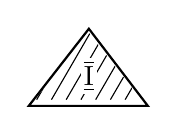
\begin{tikzpicture}[x=0.72cm,y=0.72cm]
  \draw[thick] (0,0)--(1.06,1.36)--(2.1,0)--cycle;
  \begin{scope}
    \clip (0.07,0.06)--(1.06,1.29)--(2.02,0.06)--cycle;
    \foreach \a in {0.14,0.4,...,1.95}{\draw[thin] (\a,0.11)--++(0.83,1.43);}
  \end{scope}
  \node[fill=white,inner sep=1pt] at (1.06,0.53) {$\overline{\underline{\mathrm{I}}}$};
\end{tikzpicture}}\endgroup
}
\end{GelfandAdjacentEvidence}
\begin{GelfandAdjacentEvidence}{GELFAND-P000950}{7}

--- example of a Grassm. simplex

There is a homeom., it even preserves the marks (numbers)
\SourceFigure{GELFAND-P000950}{preserved-segments}{The word before “(numbers)” reads “marks”.}
\end{GelfandAdjacentEvidence}
\begin{GelfandAdjacentEvidence}{GELFAND-P000950}{8}


$\forall$ edge --- a simplex in $G_1^1$

(7) \underline{Example}. (another one !!).

$G_2^1$

\SourceFigure{GELFAND-P000950}{dual-orbit-diagram}{Pencils through three points, a sloping transversal, and hatching. The faint lines are drawn approximately.
\par\smallskip
\begingroup\color{black}\GelfandFitDiagram{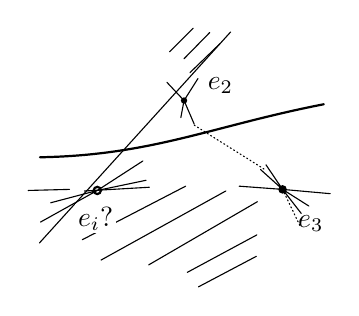
\begin{tikzpicture}[x=0.68cm,y=0.68cm,line cap=round]
  \coordinate (a) at (-1.45,0);
  \coordinate (b) at (0.17,1.68);
  \coordinate (c) at (2.01,0.02);
  \draw[thick] (-2.52,0.62) to[out=1,in=191] (2.78,1.61);
  \draw[thin] (-2.53,-0.98)--(1.04,2.96);
  \draw[thin] (-2.74,0)--(-1.97,0.02) (-1.69,-0.01)--(-0.48,0.06)
     (1.2,0.08)--(2.01,0.02)--(2.9,-0.06);
  \draw (-2.51,-0.59)--(a)--(-0.6,0.55) (-2.32,-0.23)--(a)--(-0.54,0.19);
  \draw (-0.15,2.02)--(b)--(0.36,1.24) (0.11,1.36)--(b)--(0.43,2.09);
  \draw (1.6,0.39)--(c)--(2.5,-0.29) (1.7,0.48)--(c)--(2.36,-0.43);
  \draw[thin,densely dotted] (0.36,1.22)--(1.68,0.39) (2.01,0.02)--(2.34,-0.67);
  \draw[thin] (-0.1,2.59)--(0.34,3.03) (0.17,2.46)--(0.65,2.95) (0.28,2.2)--(0.84,2.74);
  \draw[thin] (-1.73,-0.92)--(0.2,0.08) (-1.38,-1.3)--(0.95,-0.01)
     (-0.49,-1.39)--(1.54,-0.21) (0.23,-1.53)--(1.53,-0.83) (0.44,-1.8)--(1.52,-1.23);
  \draw[thick] (a) circle[radius=1.3pt];
  \fill (b) circle[radius=1.15pt] (c) circle[radius=1.55pt];
  \node[below,inner sep=1pt,fill=white] at (-1.48,-0.25) {$e_i?$};
  \node[right,inner sep=2pt] at (0.5,1.96) {$e_2$};
  \node[below right,inner sep=1pt] at (2.24,-0.4) {$e_3$};
\end{tikzpicture}}\endgroup
}
\end{GelfandAdjacentEvidence}
\begin{GelfandAdjacentEvidence}{GELFAND-P000950}{9}

\Unclear{GELFAND-P000950}{dual-left-index}{The label at the lower left is tentatively $e_i$; the index may be $1$.}
\end{GelfandAdjacentEvidence}
\begin{GelfandAdjacentEvidence}{GELFAND-P000950}{10}


orbit of a line --- $\forall$ lines which do not inters. the hatched region

This is a $\Delta$-gon --- with sides ---\par
--- lines passing through the vertices

\SourceFigure{GELFAND-P000950}{inverted-triangle}{Inverted triangle marked $13$, $23$, and circled $12$.
\par\smallskip
\begingroup\color{black}\GelfandFitDiagram{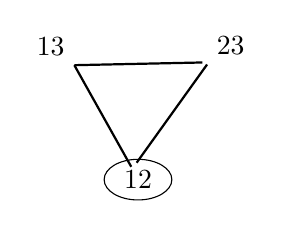
\begin{tikzpicture}[x=0.86cm,y=0.86cm]
  \draw[thick] (0,1.63)--(1.89,1.67) (1.96,1.64)--(0.92,0.19) (0.84,0.13)--(0,1.63);
  \node[above left] at (0,1.63) {$13$};
  \node[above right] at (1.96,1.64) {$23$};
  \draw (0.94,-0.06) ellipse (0.5 and 0.3);
  \node at (0.94,-0.06) {$12$};
\end{tikzpicture}}\endgroup
}
\end{GelfandAdjacentEvidence}
\begin{GelfandAdjacentEvidence}{GELFAND-P000950}{11}

--- corresp. to the side passing through $e_1$ and $e_2$.

\SourceFigure{GELFAND-P000950}{small-triangle-curves}{Triangle marked $13$ with curves crossing its sides. The faint curves are drawn approximately.
\par\smallskip
\begingroup\color{black}\GelfandFitDiagram{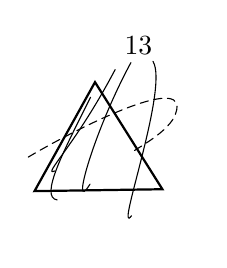
\begin{tikzpicture}[x=0.8cm,y=0.8cm,line cap=round]
  \draw[thick] (0,0)--(0.96,1.73)--(2.03,0.03)--cycle;
  \draw[thin] (0.36,-0.14) .. controls (0.07,-0.1) and (0.47,0.65) .. (0.89,1.49);
  \draw[thin] (0.32,0.32) .. controls (0.11,0.23) and (0.65,0.73) .. (1.28,1.93);
  \draw (0.88,0.11) .. controls (0.56,-0.41) and (0.93,0.93) .. (1.53,2.04);
  \draw (1.54,-0.39) .. controls (1.26,-0.77) and (2.14,1.65) .. (1.88,2.06);
  \draw[thin,densely dashed] (-0.1,0.54) .. controls (0.71,1.02) and (2.6,1.97) .. (2.21,1.16)
    .. controls (2.07,0.93) and (1.75,0.75) .. (1.58,0.64);
  \node[above] at (1.65,2.01) {$13$};
\end{tikzpicture}}\endgroup
}
\end{GelfandAdjacentEvidence}


\uwave{Sides \mbox{\(\in G_1^1\)}} $\subset G_2^1$

$\Delta_2^1$ --- inters. of the cube with the plane $\sum x_i=2$, with the vertices also denoted by pairs.

\Needspace{7\baselineskip}
\begin{GelfandAdjacentEvidence}{GELFAND-P000951}{1}
\SourcePage{GELFAND-P000951}{52}

(8) \underline{Interesting} \underline{example} $G_2^2$ \underline{or} $\Delta_2^2$

[crossed out in the left margin: \sout{(9)} (?)]
\Unclear{GELFAND-P000951}{margin-top-cancellation}{The upper crossed-out mark resembles “(9)”; “(8)” is also possible.}
\end{GelfandAdjacentEvidence}
\begin{GelfandAdjacentEvidence}{GELFAND-P000951}{2}

\[
 \sum_1^4 x_i=2\quad-\quad(\perp\ \text{main diag. section of a 4-dim. cube})
\]

[crossed out in the left margin: sign unresolved]
\Unclear{GELFAND-P000951}{margin-diagram-cancellation}{Several strokes obscure the sign to the left of the figure.}
\end{GelfandAdjacentEvidence}
\begin{GelfandAdjacentEvidence}{GELFAND-P000951}{3}

\SourceFigure{GELFAND-P000951}{diagram-delta}{Labelled sketch of $\Delta_2^2$. The faint interior connections are drawn approximately.
\par\smallskip
\begingroup\color{black}\GelfandFitDiagram{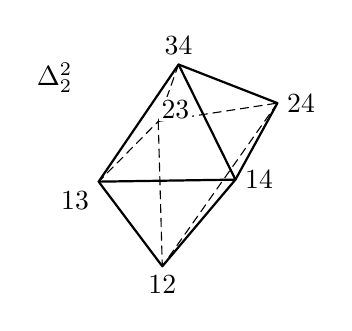
\begin{tikzpicture}[x=0.86cm,y=0.86cm,line join=round,line cap=round]
  \coordinate (t) at (0,3);
  \coordinate (u) at (1.46,2.43);
  \coordinate (v) at (0.84,1.3);
  \coordinate (w) at (-0.24,0.02);
  \coordinate (q) at (-1.18,1.27);
  \coordinate (h) at (-0.3,2.16);
  \draw[thick] (t)--(u)--(v)--(w)--(q)--cycle;
  \draw[thick] (q)--(v)--(t);
  \draw[densely dashed,thin] (t)--(h)--(q) (h)--(u) (h)--(w) (u)--(w);
  \node[above] at (t) {$34$};
  \node[right] at (u) {$24$};
  \node[right] at (v) {$14$};
  \node[below] at (w) {$12$};
  \node[below left] at (q) {$13$};
  \node[above right,fill=white,inner sep=1pt] at (h) {$23$};
  \node at (-1.83,2.8) {$\Delta_2^2$};
\end{tikzpicture}}\endgroup
}
\end{GelfandAdjacentEvidence}
\begin{GelfandAdjacentEvidence}{GELFAND-P000951}{4}


\begin{gather*}
 G_2^2\quad-\quad\text{4-dimensional}\\
 H^0\quad-\quad\text{3-dimensional}.
\end{gather*}

\SourceFigure{GELFAND-P000951}{diagram-four-planes}{Sketch with points $e_1,e_2,e_3,e_4$ and label $\ell$. The faint broken strokes are drawn approximately.
\par\smallskip
\begingroup\color{black}\GelfandFitDiagram{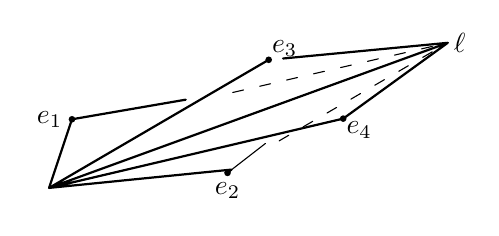
\begin{tikzpicture}[x=0.83cm,y=0.83cm,line join=round,line cap=round]
  \coordinate (o) at (0,0);
  \coordinate (e1) at (0.35,1.05);
  \coordinate (e2) at (2.73,0.23);
  \coordinate (e3) at (3.36,1.96);
  \coordinate (e4) at (4.5,1.06);
  \coordinate (l) at (6.1,2.22);
  \draw[thick] (o)--(e1)--(2.09,1.35);
  \draw[thick] (o)--(e3) (3.58,1.98)--(l) (o)--(l) (o)--(e4)--(l) (o)--(2.79,0.28)--(e2);
  \draw[thin] (e2)--(3.31,0.68);
  \draw[thin,dash pattern=on 4pt off 6pt] (2.81,1.46)--(l) (3.52,0.72)--(l);
  \foreach \point in {e1,e2,e3,e4}{\fill (\point) circle[radius=1.2pt];}
  \node[left] at (e1) {$e_1$};
  \node[below] at (e2) {$e_2$};
  \node[above right,inner sep=1pt] at (e3) {$e_3$};
  \node[below right,inner sep=1pt] at (e4) {$e_4$};
  \node[right,inner sep=2pt] at (l) {$\ell$};
\end{tikzpicture}}\endgroup
}
\end{GelfandAdjacentEvidence}
\begin{GelfandAdjacentEvidence}{GELFAND-P000951}{5}


$K(\ell)=\text{cross-ratio}$ of 4 planes\par
\hspace{2em}(anharm. ratio) \quad passing through $\ell$ and the sel. points

(take the quotient of everything by $\ell$ $\Rightarrow$ get it in the plane)
\[
 H^0\text{-orbit}\ \subset\ K(\ell)=\mathrm{const}
\]

\[
 \begin{array}{cc}
  \begin{gathered}
   G_2^2\\
   \cup\\
   G_2^2\supset
  \end{gathered}
  &
  \left\{\begin{array}{ccc|c}
   12&13&14&1\\
   21&23&24&2\\
   31&32&34&3\\
   41&42&43&4
  \end{array}\right.\\
  &\rule{11em}{0.3pt}\\
  \begin{gathered}
   G_2^1\supset\\
   \cap\\
   G_2^2
  \end{gathered}
  &
  \left\{\begin{array}{ccc|c}
   14&42&21&\phantom{1}\\
   13&32&21&\\
   14&43&31&\\
   24&43&32&
  \end{array}\right.
 \end{array}
\]
\SourceFigure{GELFAND-P000951}{table-upper-annotation}{Both upper labels read $G_2^2$, with a U-shaped sign between them.}
\end{GelfandAdjacentEvidence}
\begin{GelfandAdjacentEvidence}{GELFAND-P000951}{6}

\SourceFigure{GELFAND-P000951}{numerical-table}{The two blocks of the manuscript table, with the order of the numbers preserved.}
\end{GelfandAdjacentEvidence}
\begin{GelfandAdjacentEvidence}{GELFAND-P000951}{7}


Each one --- in its own [abbreviation unresolved] $K(\ell)=\mathrm{const}$
\Unclear{GELFAND-P000951}{below-table-abbreviation}{The abbreviation after “its own” is tentatively read as “мн-зии”. Its exact expansion is unresolved.}
\end{GelfandAdjacentEvidence}
\begin{GelfandAdjacentEvidence}{GELFAND-P000951}{8}


(9) \underline{Theorem}. The volume of the set, encl., between 2 Grassm. simplices
\[
 K(\ell)=c_1,\quad K(\ell)=c_2
\]
equals
\[
 \Phi(c_1)-\Phi(c_2),
\]
\Unclear{GELFAND-P000951}{theorem-phi-difference}{The second $\Phi$ is retraced. Its earlier form is unresolved.}
\end{GelfandAdjacentEvidence}

where
\[
 \Phi(x)=L_1(x)-L_1(1-x),\quad
 L_1(x)=\sum_{n=1}^{\infty}\frac{x^n}{n^2},\quad 0<c_1<c_2<1
\]
\hspace{6em}(integr. logarithm)

\Needspace{7\baselineskip}
\begin{GelfandAdjacentEvidence}{GELFAND-P000952}{1}
\SourcePage{GELFAND-P000952}{unlabelled}

(10) \underline{Theorem}. Generally speaking, [inserted above the line: combinatorial] homeomorphism
\SourceFigure{GELFAND-P000952}{combinatorial-insertion}{“Combinatorial” is above the line, linked by a curved mark to the start of “homeomorphism”.}
\end{GelfandAdjacentEvidence}
\begin{GelfandAdjacentEvidence}{GELFAND-P000952}{2}

\[
 \Delta_n^m\hookrightarrow \text{Grassm. complex }G_n^m
\]
preserves a number of further structures.

(11) [crossed out: \underline{\sout{Theorem}}]
\SourceFigure{GELFAND-P000952}{theorem-cancellation}{The underlined word “Theorem” remains legible beneath the hatching.}
\end{GelfandAdjacentEvidence}
\begin{GelfandAdjacentEvidence}{GELFAND-P000952}{3}

\SourceFigure{GELFAND-P000952}{faces-orbits-diagram}{Correspondence of faces and $H^0$-orbits. The stroke under “orbits” has no visible arrowhead.
\par\smallskip
\begingroup\color{black}\GelfandFitDiagram{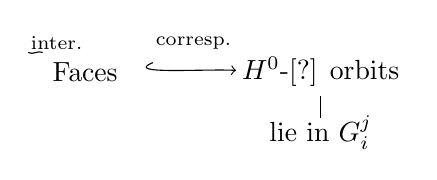
\begin{tikzpicture}[x=0.82cm,y=0.82cm]
  \node (faces) at (0,0) {Faces};
  \node[above left,inner sep=0.8pt] (interior) at (faces.north) {\scriptsize inter.};
  \draw[thin] (interior.south west) to[out=-30,in=155] (faces.north west);
  \node (orbits) at (3.65,0) {$H^0$-[?] orbits};
  \draw[->] (1.05,0.14) to[out=202,in=177] (2.34,0.02);
  \node[above] at (1.68,0.2) {\scriptsize corresp.};
  \draw (orbits.south)--++(0,-0.34);
  \node[below,inner sep=1pt] at (3.65,-0.63) {lie in $G_i^j$};
\end{tikzpicture}}\endgroup
}
\end{GelfandAdjacentEvidence}
\begin{GelfandAdjacentEvidence}{GELFAND-P000952}{4}

\Unclear{GELFAND-P000952}{faces-orbits-cancellation}{The crossed-out entry after $H^0$ and the hyphen is unresolved.}
\end{GelfandAdjacentEvidence}
\begin{GelfandAdjacentEvidence}{GELFAND-P000952}{5}


(12)
\begin{align*}
 \partial[\Delta_n^m]
 &=\sum_{i=1}^{n+m}(-1)^i\bigl\{[\Delta_n^{m-1}]\mid i\text{-th coord.}=0\bigr\}-\\
 &-\sum_{-1}^{n+m}(-1)^i\bigl\{[\Delta_{n-1}^{m}]
\end{align*}
\Incomplete{GELFAND-P000952}{boundary-formula-second-line}{The lower limit in the second sum reads $-1$. The entry breaks off after $[\Delta_{n-1}^{m}]$.}
\end{GelfandAdjacentEvidence}
\begin{GelfandAdjacentEvidence}{GELFAND-P000952}{6}


(13) \underline{Theorem}. $\forall$ harm. form in $G_n^m$ vanishes on any Grassm. simplex.

The metric is ass. to be compatible in some way with the coordinates.

\SourceFigure{GELFAND-P000952}{metric-diagram}{A brace under the list leads to the basis. The stroke below “metric” has no visible arrowhead.
\par\smallskip
\begingroup\color{black}\GelfandFitDiagram{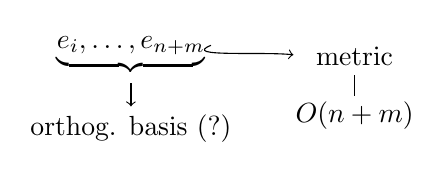
\begin{tikzpicture}[x=0.8cm,y=0.8cm]
  \node (coords) at (0,0) {$\underbrace{e_i,\ldots,e_{n+m}}$};
  \node (metric) at (3.55,0) {metric};
  \draw[->] (1.27,0.17) to[out=202,in=174] (2.58,0.02);
  \draw[->] (0,-0.43)--(0,-0.8);
  \node[below,inner sep=1pt] at (0,-0.88) {orthog. basis (?)};
  \draw (metric.south)--++(0,-0.34);
  \node[below,inner sep=1pt] at (3.55,-0.68) {$O(n+m)$};
\end{tikzpicture}}\endgroup
}
\end{GelfandAdjacentEvidence}
\begin{GelfandAdjacentEvidence}{GELFAND-P000952}{7}

\SourceFigure{GELFAND-P000952}{metric-first-index}{The first $e$ has a dotted subscript $i$.}
\end{GelfandAdjacentEvidence}
\begin{GelfandAdjacentEvidence}{GELFAND-P000952}{8}

\Unclear{GELFAND-P000952}{metric-basis-abbreviation}{The abbreviation is tentatively “orthog.”; “orthon.” is also possible.}
\end{GelfandAdjacentEvidence}
\begin{GelfandAdjacentEvidence}{GELFAND-P000952}{9}


\underline{On Atiyah’s work.}
\SourceFigure{GELFAND-P000952}{atiyah-name}{The manuscript spells the name “Атьи”.}
\end{GelfandAdjacentEvidence}
\begin{GelfandAdjacentEvidence}{GELFAND-P000952}{10}

\uwave{Hence the funct. eq. for the dilogarithm}.

Space of 5-tuples of points on $P^1$ up to proj. transf.
\SourceFigure{GELFAND-P000952}{five-points-line}{Line with five labels and an unlabelled tick on the right. The darkened end is drawn approximately.
\par\smallskip
\begingroup\color{black}\GelfandFitDiagram{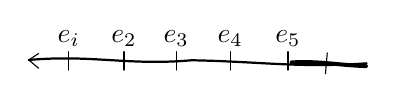
\begin{tikzpicture}[x=0.78cm,y=0.78cm,line cap=round]
  \draw[thick] (0,0.015) to[out=5,in=185] (2.65,0.01) to[out=-1,in=184] (5.5,-0.04);
  \draw (0.16,0.12)--(0,0.015)--(0.16,-0.12);
  \foreach \position/\pointindex in {0.65/i,1.55/2,2.4/3,3.28/4,4.22/5}{
    \draw (\position,-0.15)--(\position,0.15);
    \node[above,inner sep=1pt] at (\position,0.18) {$e_{\pointindex}$};
  }
  \draw[line width=1.45pt] (4.28,-0.025) to[out=3,in=178] (5.49,-0.085);
  \draw (4.83,-0.21)--(4.86,0.13);
\end{tikzpicture}}\endgroup
}
\end{GelfandAdjacentEvidence}
\begin{GelfandAdjacentEvidence}{GELFAND-P000952}{11}

\SourceFigure{GELFAND-P000952}{five-points-first-index}{The first $e$ is labelled with a dotted $i$.}
\end{GelfandAdjacentEvidence}
\begin{GelfandAdjacentEvidence}{GELFAND-P000952}{12}

This space is 2-dimensional.

\begin{align*}
 k_1&=\text{X ratio}\;(e_2\,e_3\,e_4\,e_5)\\
 k_2&=\text{--- '' ---}\;(e_1\,e_3\,e_4\,e_5)
\end{align*}
\Unclear{GELFAND-P000952}{cross-ratio-sign}{The sign before “ratio” is tentatively read as $X$. The shapes of $X$ and $\times$ are close.}
\end{GelfandAdjacentEvidence}

$\cdots$
\[
 \varphi(x)=\operatorname{Li}(x)-\operatorname{Li}(1-x),\qquad
 \operatorname{Li}(x)=\sum_1^\infty\frac{x^n}{n^2}.
\]

\begin{equation*}
 0=d\varphi(k_1)-d\varphi(k_2)+d\varphi(k_3)-d\varphi(k_4)+d\varphi(k_5)
 \tag{14}
\end{equation*}
(Funct. eq. for the dilogarithm)

This follows from the previously formul. theorems.

$G_3^2$ --- 3-dim. planes in $\mathbb R^5$.

Consider $P_1(\xi)$ (1st Pontryagin class of the tautol. 2- or 3-dim. bundle on the Grassm. $G_3^2$).

There is exactly 1 harm. 4-form.

\Needspace{7\baselineskip}
\begin{GelfandAdjacentEvidence}{GELFAND-P000953}{1}
\SourcePage{GELFAND-P000953}{53}

\[
 \underset{\substack{\Vert\\0}}{d}\pi_*P_1(\xi)
 =\pi_*\underset{\substack{\Vert\\0}}{d}P_1(\xi)
 +\sum\pi_{i*}^{\partial}P_1(\xi)
\]
\SourceFigure{GELFAND-P000953}{zeros-under-formula}{Two strokes and a zero appear below each of the two $d$ symbols.}
\end{GelfandAdjacentEvidence}
\begin{GelfandAdjacentEvidence}{GELFAND-P000953}{2}

$C$ --- space of 5-tuples of points

\SourceFigure{GELFAND-P000953}{top-projection}{The sign to the left of $\subset$ resembles lowercase $u$; uppercase $U$ is also possible.
\par\smallskip
\begingroup\color{black}\GelfandFitDiagram{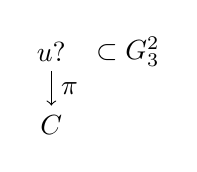
\begin{tikzpicture}[x=0.83cm,y=0.83cm]
  \node (u) at (0,0) {$u?$};
  \node at (1.17,0) {$\subset G_3^2$};
  \node (c) at (0,-1.12) {$C$};
  \draw[->] (u.south)--node[right] {$\pi$} (c.north);
\end{tikzpicture}}\endgroup
}
\end{GelfandAdjacentEvidence}
\begin{GelfandAdjacentEvidence}{GELFAND-P000953}{3}


The last term is calc. with the aid of combinatorics
\SourceFigure{GELFAND-P000953}{combinatorics-wording}{The words before “combinatorics” read “with the aid of”.}
\end{GelfandAdjacentEvidence}
\begin{GelfandAdjacentEvidence}{GELFAND-P000953}{4}


\underline{Generalization}.

Let $(\mathbb C^*)^n$ act algebraically on a homogeneous algebr. [crossed out: entry unresolved] space with a fixed point
\Incomplete{GELFAND-P000953}{generalization-cancellation}{The entry between “algebr.” and “space” is heavily crossed out.}
\end{GelfandAdjacentEvidence}
\begin{GelfandAdjacentEvidence}{GELFAND-P000953}{5}


Then

1) $\forall$ orbit of $\bigl((\mathbb R^+)^*\bigr)^n$ is homeom. to a polyhedron.
(theorem on toric embeddings)

(Diffeom. on $\forall$ orbit, but at the vertices it may have $\infty$ curvature; on the whole space --- only a homeom.)

2) $\forall$ harm. form [crossed out: entry unresolved]
invar. under $T^n\subset(\mathbb C^*)^n$
\Incomplete{GELFAND-P000953}{harmonic-cancellation}{Several strokes obscure the entry after “form”.}
\end{GelfandAdjacentEvidence}
\begin{GelfandAdjacentEvidence}{GELFAND-P000953}{6}

[inserted below “harm. form”: (with respect to $\forall$ Kähler metric)]
\SourceFigure{GELFAND-P000953}{kahler-insertion}{The condition on the metric is written on the line below.}
\end{GelfandAdjacentEvidence}
\begin{GelfandAdjacentEvidence}{GELFAND-P000953}{7}

is equal to $0$ on $\forall$ $\bigl((\mathbb R^+)^*\bigr)^n$-orbit.

(15) \underline{Theorem}. (Atiyah).

$M$ --- symplect. manif., $f_1,\ldots,f_n\colon M\longrightarrow\mathbb R$ functions.
\SourceFigure{GELFAND-P000953}{symplectic-abbrev}{The Russian abbreviation after “symplect.” reads “мн-зие” (manifold).}
\end{GelfandAdjacentEvidence}
\begin{GelfandAdjacentEvidence}{GELFAND-P000953}{8}

\[
 \{f_i,f_j\}=0
\]

$df_i$ all vanish to $0$ at \underline{some point}.

We get a map
\[
 M\underset{f_1,\ldots,f_n}{\longrightarrow}\mathbb R^n
\]
Here

\SourceFigure{GELFAND-P000953}{orbit-image}{An arrow leads from $O$ to the convex set. A stroke below $O$ leads to the orbit label.
\par\smallskip
\begingroup\color{black}\GelfandFitDiagram{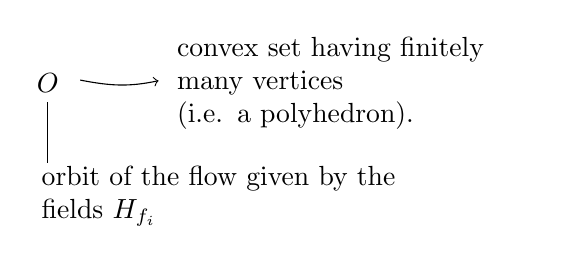
\begin{tikzpicture}[x=0.79cm,y=0.79cm]
  \node (orb) at (0,0) {$O$};
  \draw[->] (0.52,0.05) to[out=-11,in=192] (1.78,0.04);
  \node[anchor=west,align=left,text width=4.7cm] (target) at (1.92,0)
    {convex set having finitely many vertices\\(i.e. a polyhedron).};
  \coordinate (flowtop) at (orb.center |- target.south);
  \node[anchor=north west,align=left,text width=5.25cm,inner sep=1pt] (flow) at ([xshift=-1.2mm,yshift=-3mm]flowtop) {orbit of the flow given by the fields $H_{f_i}$};
  \draw (orb.south)--(orb.south |- flow.north);
\end{tikzpicture}}\endgroup
}
\end{GelfandAdjacentEvidence}
\begin{GelfandAdjacentEvidence}{GELFAND-P000953}{9}


\SourceFigure{GELFAND-P000953}{divider-strokes}{Two strokes with a dot between them.
\par\smallskip
\begingroup\color{black}\GelfandFitDiagram{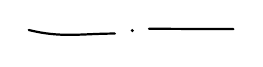
\begin{tikzpicture}[x=0.76cm,y=0.76cm,line cap=round]
  \draw[thick] (0,0.06) to[out=-14,in=180] (1.44,0);
  \fill (1.73,0.05) circle[radius=0.62pt];
  \draw[thick] (2.01,0.08)--(3.42,0.075);
\end{tikzpicture}}\endgroup
}
\end{GelfandAdjacentEvidence}


\underline{Problem}: relation to integr. by quadratures.

\clearpage
\pdfbookmark[0]{Chapter 19}{gelfand-archive-chapter-19}
\section*{Chapter 19}
\Needspace{7\baselineskip}
\begin{GelfandAdjacentEvidence}{GELFAND-P000954}{1}
\SourcePage{GELFAND-P000954}{unlabelled}

16/\(\overline{\underline{\mathrm{II}}}\)-81.\quad \underline{Gelfand Sem.}
\SourceFigure{GELFAND-P000954}{date-hatching}{A narrow hatched bar underlines the date. II has a stroke above and below it.
\par\smallskip
\begingroup\color{black}\GelfandFitDiagram{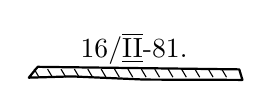
\begin{tikzpicture}[x=0.81cm,y=0.81cm,line join=round]
  \node[above,inner sep=2pt] at (1.65,0.11) {16/\(\overline{\underline{\mathrm{II}}}\)-81.};
  \draw[thick] (0,0)--(0.14,0.17)--(3.3,0.13)--(3.35,-0.035)--(1.82,-0.03)--(0.67,0.02)--cycle;
  \foreach \x in {0.16,0.37,...,3.2}{\draw[thin] (\x,0.008)--++(-0.075,0.127);}
\end{tikzpicture}}\endgroup
}
\end{GelfandAdjacentEvidence}
\begin{GelfandAdjacentEvidence}{GELFAND-P000954}{2}


\underline{\underline{Khovanskii}}. \quad \underline{On Newton polyhedra}.

[At the right: (reverse side of the prev. talk by Mc Pherson.)]
\SourceFigure{GELFAND-P000954}{verso-note}{The note identifies this as the reverse side of the preceding talk.}
\end{GelfandAdjacentEvidence}
\begin{GelfandAdjacentEvidence}{GELFAND-P000954}{3}


$\underline{\underline{n=2}}$ \uwave{for simplicity}.

\underline{refs.}: 1) Mumford et al. Lect. Notes --- toric embeddings.

2) D. Bernstein, FA.

1) Kempf, Knudsen, Mumford, Saint-Donat, Toroidal Embeddings,

Lect. Notes Math., 1972, $N=339$.
\SourceFigure{GELFAND-P000954}{printed-year}{The manuscript citation gives the year 1972 and number 339.}
\end{GelfandAdjacentEvidence}


\Needspace{7\baselineskip}
\begin{GelfandAdjacentEvidence}{GELFAND-P000955}{1}
\SourcePage{GELFAND-P000955}{unlabelled}

and also a survey by \uwave{Danilov} in UMN.

Articles by \uwave{Khovanskii}: FA, 1977, 11:4\par
\hspace{4em}1978, 12:1

\begin{equation*}
 \{(x,y):P(x,y)=0\}
 \tag{1}
\end{equation*}
what does this curve look like? (handles, etc.)

How many solutions does the system have
\begin{equation*}
 \begin{cases}
 P(x,y)=0\\
 Q(x,y)=0
 \end{cases}
 \tag{2}
\end{equation*}
[crossed out: (line unresolved).]
\Incomplete{GELFAND-P000955}{cancelled-line}{The parenthetical line is heavily crossed out.}
\end{GelfandAdjacentEvidence}
\begin{GelfandAdjacentEvidence}{GELFAND-P000955}{2}


\begin{equation*}
 y^2=P_n(x)
 \tag{3}
\end{equation*}
has $\sim n/2$ handles (more precisely, $\left[\frac{n-1}{2}\right]$ handles).
\begin{gather*}
 n=3,4\qquad 1\text{ handle},\\
 n=5,6\qquad 2\text{ handles}.
\end{gather*}
Condition: $P_n$ has no multiple roots.

For a general eq. (1) there is also a recipe for computing the number of handles:
\begin{equation*}
 \frac{(n-1)(n-2)}{2}\qquad\text{\uwave{for an eq. in general position.}}
 \tag{4}
\end{equation*}
(3) --- is not an eq. of degree $n$ in fact.
\SourceFigure{GELFAND-P000955}{degree-remark}{The sentence about the degree in (3) follows the manuscript wording.}
\end{GelfandAdjacentEvidence}
\begin{GelfandAdjacentEvidence}{GELFAND-P000955}{3}


It all comes down to the Newton polyh..
\begin{equation*}
 P(x,y)=\sum a_{n,k}x^n y^k.
 \tag{5}
\end{equation*}
\SourceFigure{GELFAND-P000955}{newton-triangle}{Hatched triangle, axes $k,n$, and marked points. The label above $2$ is crossed out.
\par\smallskip
\begingroup\color{black}\GelfandFitDiagram{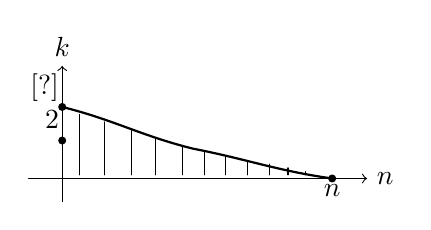
\begin{tikzpicture}[x=0.79cm,y=0.79cm,line cap=round]
  \draw[->] (-0.54,0)--(4.9,0) node[right] {$n$};
  \draw[->] (0,-0.37)--(0,1.81) node[above] {$k$};
  \draw[thick] (0,1.15) to[out=-14,in=166] (2.1,0.48) to[out=-11,in=172] (4.34,0);
  \foreach \x/\h in {0.28/1.03,0.68/0.91,1.12/0.77,1.5/0.65,1.94/0.53,2.29/0.44,2.63/0.36,2.98/0.29,3.33/0.23,3.63/0.17,3.91/0.11}{
    \draw[thin] (\x,0.06)--(\x,\h);
  }
  \fill (0,0.61) circle[radius=1.45pt] (0,1.15) circle[radius=1.45pt] (4.34,0) circle[radius=1.45pt];
  \node[below left,inner sep=1pt] at (0,1.15) {$2$};
  \node[left,inner sep=1pt] at (0,1.46) {$[\text{?}]$};
  \node[below,inner sep=2pt] at (4.34,0) {$n$};
\end{tikzpicture}}\endgroup
}
\end{GelfandAdjacentEvidence}
\begin{GelfandAdjacentEvidence}{GELFAND-P000955}{4}

\Incomplete{GELFAND-P000955}{triangle-cancelled-label}{The heavily crossed-out label above $2$ is unresolved.}
\end{GelfandAdjacentEvidence}
\begin{GelfandAdjacentEvidence}{GELFAND-P000955}{5}


\uwave{Convex hull} of those $(n,k)$, for which $a_{nk}\ne0$.

\SourceFigure{GELFAND-P000955}{general-simplex}{The second triangle, with four interior strokes.
\par\smallskip
\begingroup\color{black}\GelfandFitDiagram{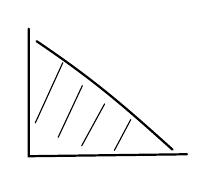
\begin{tikzpicture}[x=0.83cm,y=0.83cm,line cap=round]
  \draw[thick] (0,1.95)--(0,0)--(2.42,0.03);
  \draw[thick] (0.12,1.76) to[out=-34,in=138] (2.2,0.1);
  \draw (0.1,0.51)--(0.52,1.43) (0.45,0.29)--(0.82,1.08)
        (0.81,0.16)--(1.16,0.8) (1.31,0.09)--(1.56,0.56);
\end{tikzpicture}}\endgroup
}
\end{GelfandAdjacentEvidence}
\begin{GelfandAdjacentEvidence}{GELFAND-P000955}{6}

--- \uwave{gen. case} --- simplex.

Answer for (1) --- [inserted above the line: \uwave{number of handles} $=$]
\uwave{number of interior lattice points in the Newton polyh.}
\SourceFigure{GELFAND-P000955}{genus-insertion}{“number of handles” and the equals sign are inserted above the answer.}
\end{GelfandAdjacentEvidence}


(for coeffs. $a_{n,k}$ in general position)

This is a theor. of \uwave{Baker} (that very one), rediscovered by Khovanskii in 1976.

(Baker taught Hodge, Hodge taught Atiyah)

In $\mathbb C^2$ some points of the curve (1) are hidden. We want to bring them out by certain substitutions.

Consid. the curve $P(x,y)=0$ \uwave{away from the coordinate cross}.

$x,y$ --- meromorphic fns. on a Riem. surface.

Sometimes they become $0$ or $\infty$. This gives a divisor:

at $\forall$ of its points there is a vector $(n,m)$

(order of the zero of $x=n$, order of the zero of $y=m$ at the given point)

\Needspace{7\baselineskip}
\begin{GelfandAdjacentEvidence}{GELFAND-P000956}{1}
\SourcePage{GELFAND-P000956}{6}

Points of order $(1,0)$ or $(k,0)$ are visible in the picture: they are the points of inters. with the axis \underline{$x=0$}.

We can transl. the polygon by multiplication by $x^k$ and $y^k$.

\SourceFigure{GELFAND-P000956}{axis-polygon}{The pentagon meets the $y$-axis along an edge and the $x$-axis at a vertex.
\par\smallskip
\begingroup\color{black}\GelfandFitDiagram{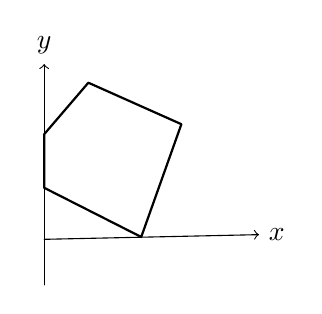
\begin{tikzpicture}[x=0.85cm,y=0.85cm,line cap=round,line join=round]
  \draw[->] (0,-0.68)--(0,2.62) node[above] {$y$};
  \draw[->] (0,0)--(3.21,0.07) node[right] {$x$};
  \draw[thick] (0,0.77)--(0,1.57)--(0.66,2.34)--(2.05,1.72)--(1.45,0.035)--cycle;
\end{tikzpicture}}\endgroup
}
\end{GelfandAdjacentEvidence}
\begin{GelfandAdjacentEvidence}{GELFAND-P000956}{2}


Translate so that it touches the axis $x=0$.
\begin{equation*}
 P(0,y)=0
 \tag{6}
\end{equation*}
Number of sols. $=$ \uwave{length of the segment of intersection} of NP with the axis $\{x=0\}$.

(if there are no multiple roots

\SourceFigure{GELFAND-P000956}{transverse-branches}{Three branches cross the vertical line labelled $x=0$.
\par\smallskip
\begingroup\color{black}\GelfandFitDiagram{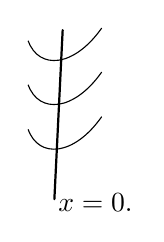
\begin{tikzpicture}[x=0.81cm,y=0.81cm,line cap=round]
  \draw[thick] (-0.07,0)--(0.06,2.65);
  \foreach \level in {0.95,1.65,2.34}{
    \draw (-0.48,\level+0.14) .. controls (-0.31,\level-0.32) and (0.24,\level-0.27) .. (0.67,\level+0.34);
  }
  \node[below right,inner sep=1pt] at (-0.06,0.14) {\uwave{\mbox{\(x=0\)}}.};
\end{tikzpicture}}\endgroup
}
\end{GelfandAdjacentEvidence}
\begin{GelfandAdjacentEvidence}{GELFAND-P000956}{3}

nonmultiple $\Rightarrow$ the implicit fn. thm. applies

$\Rightarrow$ there are no points of the form $(k,0)$, $k\geqslant2$.

\uwave{Make a transf.}
\begin{equation*}
 \begin{cases}
 x=u^{a_{11}}v^{a_{12}},\\
 y=u^{a_{21}}v^{a_{22}},
 \end{cases}
 \qquad a_{ij}\in\mathbb Z
 \tag{7}
\end{equation*}
\begin{equation*}
 \det\begin{Vmatrix}a_{11}&a_{12}\\a_{21}&a_{22}\end{Vmatrix}=1,
 \qquad A=\begin{pmatrix}a_{11}&a_{12}\\a_{21}&a_{22}\end{pmatrix}.
 \tag{8}
\end{equation*}
the inverse is integer-valued $\Rightarrow$ there is an inverse transf. (also rational)

If $u\sim t^m$, $v\sim t^n$, then after the transformation
\begin{equation*}
 \operatorname{ord}\left(\text{[crossed out]}\ \begin{matrix}x\\y\end{matrix}\right)
 =A\ \text{[crossed out]}\begin{pmatrix}m\\n\end{pmatrix}.
 \tag{9}
\end{equation*}
\Unclear{GELFAND-P000956}{order-formula}{The signs left of the column $x,y$ and after $A$ are heavily crossed out. Both resemble $u$, but the exact reading is unresolved.}
\end{GelfandAdjacentEvidence}
\begin{GelfandAdjacentEvidence}{GELFAND-P000956}{4}


We want a transf. such that at the pt. $\binom{n}{m}$ there lands $\binom{1}{0}$.

Let the vector $(n,m)$ be primitive ($\sim$ on the segment $[0,(m,n)]$ there are no lattice points).
\Unclear{GELFAND-P000956}{primitive-vector}{The first character of the pair is heavily retraced and tentatively read as $n$. The next entry has the order $(m,n)$.}
\end{GelfandAdjacentEvidence}
\begin{GelfandAdjacentEvidence}{GELFAND-P000956}{5}


\uwave{Moral}: $\exists$ a matrix $A$.

If [crossed out: \sout{it} (?); inserted above the line: $(n,m)$] is reducible, then this same transf. shows that \underline{there are no such divisors}!!
\Unclear{GELFAND-P000956}{substituted-vector}{Above the crossed-out word, tentatively “it”, is the insertion $(n,m)$.}
\end{GelfandAdjacentEvidence}
\begin{GelfandAdjacentEvidence}{GELFAND-P000956}{6}


\underline{answer}.

\SourceFigure{GELFAND-P000956}{vertex-support}{One of the parallel lines meets a vertex of the pentagon. An arrow labelled $(n,m)$ starts at the marked point on the other line.
\par\smallskip
\begingroup\color{black}\GelfandFitDiagram{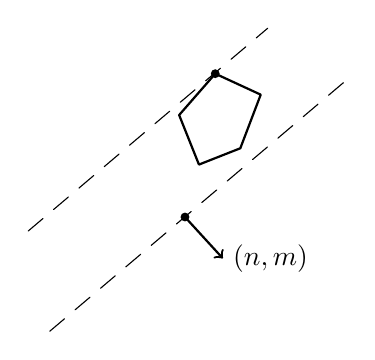
\begin{tikzpicture}[x=0.74cm,y=0.74cm,line cap=round,line join=round]
  \coordinate (v) at (1.55,2.67);
  \coordinate (o) at (1.03,0.21);
  \draw[thin,dash pattern=on 7pt off 5pt] (-1.66,-0.03)--(2.45,3.45);
  \draw[thick] (v)--(2.33,2.31)--(1.98,1.39)--(1.27,1.11)--(0.93,1.96)--cycle;
  \draw[thin,dash pattern=on 7pt off 5pt] (-1.29,-1.75)--(3.79,2.55);
  \fill (v) circle[radius=1.6pt] (o) circle[radius=1.6pt];
  \draw[thick,->] (o)--(1.68,-0.5) node[right] {$(n,m)$};
\end{tikzpicture}}\endgroup
}
\end{GelfandAdjacentEvidence}
\begin{GelfandAdjacentEvidence}{GELFAND-P000956}{7}


\uwave{move it until it touches}

[crossed out: \sout{if} (?)] We hit a point ---\par
--- then there are none of this kind.
\Unclear{GELFAND-P000956}{cancelled-word}{The crossed-out word is tentatively read as “if”.}
\end{GelfandAdjacentEvidence}
\begin{GelfandAdjacentEvidence}{GELFAND-P000956}{8}


\SourceFigure{GELFAND-P000956}{edge-support}{The left edge of the hexagon is emphasized on a sloping line. A parallel line is to the right.
\par\smallskip
\begingroup\color{black}\GelfandFitDiagram{\begin{tikzpicture}[x=0.74cm,y=0.74cm,line cap=round,line join=round]
  \coordinate (a) at (0.18,0.81);
  \coordinate (b) at (0.82,1.92);
  \draw[thin] (-0.73,-0.78)--(b);
  \draw[thin,dash pattern=on 8pt off 6pt] (1.74,-1.06)--(3.82,2.54);
  \draw[thick] (a)--(b)--(1.85,2.04)--(2.58,1.46)--(1.94,0.36)--(1.17,0.28)--cycle;
  \draw[line width=1.2pt] (a)--(b);
\end{tikzpicture}}\endgroup
}
\end{GelfandAdjacentEvidence}
\begin{GelfandAdjacentEvidence}{GELFAND-P000956}{9}

$\leftarrow$ then we get $=$ the number of lattice points on this segment.
\SourceFigure{GELFAND-P000956}{final-count}{The last line gives “the number of lattice points on this segment”.}
\end{GelfandAdjacentEvidence}


(take the $\min$ of the scalar product)

\Needspace{7\baselineskip}
\begin{GelfandAdjacentEvidence}{GELFAND-P000957}{1}
\SourcePage{GELFAND-P000957}{unlabelled}

\uwave{Total number of punctures} $=$ the number of lattice points on the boundary.

Consider now the system
\begin{equation*}
 \begin{cases}
 P(x,y)=0\\
 Q(x,y)=0
 \end{cases}
 \tag{10}
\end{equation*}
and seek the number of sols. in $(\mathbb C\setminus0)^2$

([crossed out: unresolved] $x\ne0,\infty$; $y\ne0,\infty$).
\Unclear{GELFAND-P000957}{cancelled-before-conditions}{A short entry before the condition on $x$ is obscured by crossing-out.}
\end{GelfandAdjacentEvidence}
\begin{GelfandAdjacentEvidence}{GELFAND-P000957}{2}


Consid. the fn. $Q$ on the curve $P(x,y)=0$.

Its divisor $=0$,
\SourceFigure{GELFAND-P000957}{divisor-zero}{The manuscript reads “Its divisor $=0$”.}
\end{GelfandAdjacentEvidence}
\begin{GelfandAdjacentEvidence}{GELFAND-P000957}{3}

Look at the order at the omitted pts.!!

$(n,m)$\qquad $x\sim t^n$, $y\sim t^m$.

Then
\begin{equation*}
 \sum C_{a,b}x^a y^b=C_{a,b}t^{an+bm}
 \tag{11}
\end{equation*}
\SourceFigure{GELFAND-P000957}{expansion-eleven}{In (11) the summation sign stands to the left of the equality.}
\end{GelfandAdjacentEvidence}
\begin{GelfandAdjacentEvidence}{GELFAND-P000957}{4}


\underline{answer}:
\begin{equation*}
 \underline{\underline{\min_{a,b}\bigl((n,m)\cdot(a,b)\bigr)}}
 \qquad\text{--- \uwave{a purely geom. answer}.}
 \tag{12}
\end{equation*}
Punctured points --- on the cross or at $\infty$

$\Rightarrow$ \uwave{poles only at the punctured points}.
\begin{equation*}
 \left[\sum_{m,n}(12)\right]
 =\text{the number of sols. of (10) in [crossed out: \sout{the space} (?)] }(\mathbb C\setminus0)^2.
 \tag{13}
\end{equation*}
\Unclear{GELFAND-P000957}{thirteen-cancellation}{The crossed-out word before $(\mathbb C\setminus0)^2$ is tentatively read as “the space”.}
\end{GelfandAdjacentEvidence}
\begin{GelfandAdjacentEvidence}{GELFAND-P000957}{5}

\SourceFigure{GELFAND-P000957}{thirteen-sign}{There is no minus sign before the summation in (13).}
\end{GelfandAdjacentEvidence}
\begin{GelfandAdjacentEvidence}{GELFAND-P000957}{6}


(for gen. pos. --- otherwise cancellation may occur).

There are 2 polygons!! What do we get?

\underline{Answer} --- mixed volume!!

Add all the vects. $(n,m)$ --- we get a vector of length $=$ the length of the side.

\SourceFigure{GELFAND-P000957}{normal-arrows}{Three successive arrows point down and to the right.
\par\smallskip
\begingroup\color{black}\GelfandFitDiagram{\begin{tikzpicture}[x=0.87cm,y=0.87cm,line cap=round]
  \draw[very thick,->] (0,1.53)--(0.24,1.02);
  \draw[very thick,->] (0.24,1.02)--(0.46,0.47);
  \draw[very thick,->] (0.46,0.47)--(0.59,-0.06);
\end{tikzpicture}}\endgroup
}
\end{GelfandAdjacentEvidence}
\begin{GelfandAdjacentEvidence}{GELFAND-P000957}{7}


A vector $\perp$ to the side and equal to it in length.

\uwave{Suppose the 2 polygons coincide} (i.e. the same nonzero coefficients! of $P$ and $Q$).
\SourceFigure{GELFAND-P000957}{same-coefficients}{The parenthesis reads “the same nonzero coefficients!”}
\end{GelfandAdjacentEvidence}
\begin{GelfandAdjacentEvidence}{GELFAND-P000957}{8}


\SourceFigure{GELFAND-P000957}{area-triangle}{Triangle with side $a$, height $h$, vertex $O$, and an outward arrow.
\par\smallskip
\begingroup\color{black}\GelfandFitDiagram{\begin{tikzpicture}[x=0.92cm,y=0.92cm,line cap=round,line join=round]
  \coordinate (a) at (0,0.66);
  \coordinate (b) at (1.91,1.42);
  \coordinate (o) at (1.17,0);
  \draw[thick] (a)--(b)--(o)--cycle;
  \foreach \v in {a,b,o}{\draw[thick,fill=white] (\v) circle[radius=1.6pt];}
  \draw (o)--(0.81,0.98) node[pos=0.56,right,inner sep=1pt] {$h$};
  \draw[thick,->] (0.67,0.93)--(0.32,2.02);
  \node[above,inner sep=1pt] at (1.47,1.28) {$a$};
  \node[right] at (1.36,-0.01) {$O$};
\end{tikzpicture}}\endgroup
}
\end{GelfandAdjacentEvidence}
\begin{GelfandAdjacentEvidence}{GELFAND-P000957}{9}


$\max$ for the triangle among all scalar prods. $=$
\SourceFigure{GELFAND-P000957}{triangle-word}{The first word reads Latin $\max$.}
\end{GelfandAdjacentEvidence}
\begin{GelfandAdjacentEvidence}{GELFAND-P000957}{10}


$=ah=2S$.

(fix $O$)

\SourceFigure{GELFAND-P000957}{bezout-triangle}{Small unlabelled right triangle.
\par\smallskip
\begingroup\color{black}\GelfandFitDiagram{\begin{tikzpicture}[x=0.82cm,y=0.82cm,line cap=round]
  \draw[thick] (0,-0.04)--(0,1.53) (0.06,1.44)--(1.44,0.01)--(0,0.04);
\end{tikzpicture}}\endgroup
}
\end{GelfandAdjacentEvidence}
\begin{GelfandAdjacentEvidence}{GELFAND-P000957}{11}

$\triangle$-gon $\Rightarrow$ we get $n^2$ (Bézout’s theor.).

\underline{Mixed area}.

\SourceFigure{GELFAND-P000957}{mixed-area-diagrams}{Hexagon and triangle with marked points. The dashed line and short strokes at the right-hand line are drawn approximately.
\par\smallskip
\begingroup\color{black}\GelfandFitDiagram{\begin{tikzpicture}[x=0.78cm,y=0.78cm,line join=round,line cap=round]
  \coordinate (a) at (0.15,0.79);
  \coordinate (b) at (0.82,1.58);
  \draw[thin] (-0.68,-0.19)--(1.24,2.08);
  \draw[thick] (a)--(b)--(2.1,1.54)--(2.24,0.69)--(1.63,0.03)--(0.34,0.04)--cycle;
  \draw[thin] (3.43,-0.76)--(5.27,1.72);
  \draw[dashed,thin] (0.56,1.34)--(3.59,-0.54);
  \draw[thin] (3.43,-0.46)--(3.66,-0.54)--(3.74,-0.56);
  \draw[thick] (4.69,1.39)--(5.99,1.67)--(5.17,0.26)--cycle;
  \fill (1.18,0.87) circle[radius=1.8pt] (5.34,1.03) circle[radius=2.05pt];
\end{tikzpicture}}\endgroup
}
\end{GelfandAdjacentEvidence}
\begin{GelfandAdjacentEvidence}{GELFAND-P000957}{12}


sides [crossed out: \sout{mult.} (?)] of one mult. by the heights of the other.
\Unclear{GELFAND-P000957}{mixed-area-word}{The crossed-out word after “sides” is tentatively read as “mult.”}
\end{GelfandAdjacentEvidence}


A common point is marked $O$.

$\forall$ side is moved until it supports the 2nd --- this is the height.

\Needspace{7\baselineskip}
\begin{GelfandAdjacentEvidence}{GELFAND-P000958}{1}
\SourcePage{GELFAND-P000958}{7}

\uwave{General defn.}

$M,N$ --- figures.
\[
 S(\alpha M+\beta N)=\alpha^2S(M)+\beta^2S(N)+
 \alpha\beta\underbrace{S(M,N)}_{\text{mixed volume.}}
\]
\SourceFigure{GELFAND-P000958}{mixed-volume-normalization}{The first equality has $S(M,N)$ as the coefficient of $\alpha\beta$. The manuscript then uses $V$.}
\end{GelfandAdjacentEvidence}
\begin{GelfandAdjacentEvidence}{GELFAND-P000958}{2}


\uwave{In} $n$-\uwave{dimensional space} --- \uwave{mixed volume} $n$ \uwave{figures}.

$V(\Delta_1,\ldots,\Delta_n)$ is def. by the properties:
\begin{align*}
 1)\quad &V(\Delta,\ldots,\Delta)=V(\Delta)\text{ --- volume.}\\
 2)\quad &V(\Delta_1+\Delta'_1,\Delta_2,\ldots)
  =V(\Delta_1,\Delta_2,\ldots)+V(\Delta'_1,\Delta_2,\ldots)
\end{align*}
Such a fn. [crossed out: entry unresolved] exists and is unique.
\Unclear{GELFAND-P000958}{existence-cancellation}{A short entry after “fn.” is crossed out.}
\end{GelfandAdjacentEvidence}
\begin{GelfandAdjacentEvidence}{GELFAND-P000958}{3}


(14) \underline{Thm.} (D. Bernstein)

\uwave{Number of sols.} (in $(\mathbb C\setminus0)^2$) \uwave{of a system in gen. pos.} \dashuline{of form} (2) $=$

$=$ \uwave{mixed volume of their Newton polyh.}.

(15) \underline{Thm.}

\uwave{Euler char.} [crossed out: \sout{of the curve} (?)] \uwave{of the hypersurf.},
$P(x)$ [crossed out: \(,y)\) (?)] \( {}=0 \)
\Unclear{GELFAND-P000958}{euler-cancellation}{The crossed-out word before “hypersurf.” is tentatively read as “of the curve”.}
\end{GelfandAdjacentEvidence}
\begin{GelfandAdjacentEvidence}{GELFAND-P000958}{4}

\Unclear{GELFAND-P000958}{euler-polynomial}{A heavily crossed-out entry follows $P(x)$, possibly \(,y)\).}
\end{GelfandAdjacentEvidence}
\begin{GelfandAdjacentEvidence}{GELFAND-P000958}{5}


(with the coord. cross removed)
\[
 =-n!\bigl(\underline{\text{volume of the Newton polyh.}}\bigr)
\]
\SourceFigure{GELFAND-P000958}{euler-sign}{A minus sign is written before $n!$.}
\end{GelfandAdjacentEvidence}
\begin{GelfandAdjacentEvidence}{GELFAND-P000958}{6}


\underline{Corollary (geom.)}
\[
 2-2B-\Gamma=-2S.
\]
$B$ --- number of interior lattice pts..

$\Gamma$ --- ---''--- boundary ---''---
\begin{equation*}
 \underline{B+\tfrac12\Gamma=S+1}.
 \tag{16}
\end{equation*}
\dashuline{Relation of mixed volume to the} \underline{isoperimetric inequality}.

\SourceFigure{GELFAND-P000958}{circle-and-polygon}{Hatched circle with radius $1$ and a hexagon.
\par\smallskip
\begingroup\color{black}\GelfandFitDiagram{\begin{tikzpicture}[x=0.84cm,y=0.84cm,line cap=round,line join=round]
  \draw[thick] (0,0) ellipse (0.72 and 0.64);
  \begin{scope}
    \clip (0,0) ellipse (0.72 and 0.64);
    \foreach \a in {-0.67,-0.41,...,0.63}{\draw[thin] (\a,-0.52)--++(0.39,1.16);}
  \end{scope}
  \fill (0,-0.06) circle[radius=1.55pt];
  \draw[->,thick] (0,-0.06)--(0.57,0.19);
  \node[above,fill=white,inner sep=0.6pt] at (0.25,0.13) {$1$};
  \draw[thick] (2.15,0)--(2.53,0.78)--(3.78,1.25)--(4.21,0.44)--(3.98,-0.42)--(2.88,-0.91)--cycle;
\end{tikzpicture}}\endgroup
}
\end{GelfandAdjacentEvidence}
\begin{GelfandAdjacentEvidence}{GELFAND-P000958}{7}

\begin{equation*}
 S(\Delta_1,\Delta_2)=S(\Delta_1+\Delta_2)-S(\Delta_1)-S(\Delta_2).
 \tag{17}
\end{equation*}
$O$ --- centre of the circle.

Mixed area of the polygon and the circle = the perimeter of the polygon.

\underline{Inequality}:
\begin{equation*}
 V^2(\Delta_1,\Delta_2)\geqslant V(\Delta_1)V(\Delta_2).
 \tag{18}
\end{equation*}
Attained on the circle.

\uwave{Theorem for any alg. surface.}

$\Gamma_1,\Gamma_2$ --- two curves on an algebr. surface.
\begin{equation*}
 (\Gamma_1,\Gamma_2)^2\geqslant(\Gamma_1,\Gamma_1)\cdot(\Gamma_2,\Gamma_2).
 \tag{19}
\end{equation*}
[label by $(\Gamma_1,\Gamma_2)$: inters. index]
\SourceFigure{GELFAND-P000958}{intersection-index-note}{A short stroke leads from the term on the left to “inters. index”.}
\end{GelfandAdjacentEvidence}
\begin{GelfandAdjacentEvidence}{GELFAND-P000958}{8}


(known from Hodge structures)
\SourceFigure{GELFAND-P000958}{intersection-hypotheses}{On this frame, (19) is accompanied by the two curves on an algebraic surface and the note on Hodge structures.}
\end{GelfandAdjacentEvidence}


\Needspace{7\baselineskip}
\begin{GelfandAdjacentEvidence}{GELFAND-P000959}{1}
\SourcePage{GELFAND-P000959}{unlabelled}

We construct a special compactif. of $(\mathbb C\setminus0)^2$.

There is a set $P(x,y)=0$.

We want to describe its charts so that the transitions are only monomial and yet it would be possible to consider everything,

what compact complex manifolds there are which are covered by a system of charts, the transition being given by unimod. matrices.

\SourceFigure{GELFAND-P000959}{cone-schematic}{Hatched cone with two labelled rays. The rays continue in broken strokes beyond the arrowheads.
\par\smallskip
\begingroup\color{black}\GelfandFitDiagram{\begin{tikzpicture}[x=0.8cm,y=0.8cm,scale=0.88,line cap=round]
 \draw[->,thick] (0,0)--(1.05,1.85);
 \draw[dashed] (1.05,1.85)--(1.48,2.61);
 \draw[->,thick] (0,0)--(2.1,0.9);
 \draw[dashed] (2.1,0.9)--(4.22,1.81);
 \draw (0.34,0.15)--(0.23,0.4) (0.7,0.30)--(0.49,0.84)
       (1.0,0.43)--(0.77,1.32) (1.34,0.57)--(1.09,1.85)
       (1.68,0.72)--(1.46,2.22) (2.0,0.86)--(1.8,2.17)
       (2.35,1.01)--(2.18,2.15) (2.69,1.15)--(2.58,2.07)
       (3.04,1.30)--(2.97,1.99) (3.39,1.45)--(3.36,1.94);
 \node[left,inner sep=1pt] at (0.64,1.30) {$(a_{11},a_{12})$};
 \node[below,inner sep=2pt] at (2.21,0.82) {$(a_{21},a_{22})$};
\end{tikzpicture}}\endgroup
}
\end{GelfandAdjacentEvidence}
\begin{GelfandAdjacentEvidence}{GELFAND-P000959}{2}

\begin{gather*}
 \begin{pmatrix}x\\y\end{pmatrix}\in\underline{\underline{\text{the torus}}}\\
 (x\ne0,y\ne0)\\
 (\mathbb C\setminus0)^2
\end{gather*}
\SourceFigure{GELFAND-P000959}{torus-notation}{The word “тору” (“the torus”) is underlined twice.}
\end{GelfandAdjacentEvidence}
\begin{GelfandAdjacentEvidence}{GELFAND-P000959}{3}


[under the figure on the left: crossed out \sout{it} (?)]
\Unclear{GELFAND-P000959}{cancelled-under-cone}{The crossed-out entry resembles “он” (“it”); the reading is unresolved.}
\end{GelfandAdjacentEvidence}
\begin{GelfandAdjacentEvidence}{GELFAND-P000959}{4}


For now it is noncompact.

With each transf. (7) we glue on $u=0$, $v=0$ [above the entry in a brace: “2 lines”] and draw a cone.
\Unclear{GELFAND-P000959}{two-lines-notation}{At the start of the brace, left of “2 lines”, there is a dark stroke. It is unclear whether a separate entry was crossed out here.}
\end{GelfandAdjacentEvidence}


If they intersect, the construction is impossible.

It is possible if the cones cover all of $\mathbb R^2$.

\Needspace{7\baselineskip}
\begin{GelfandAdjacentEvidence}{GELFAND-P000960}{1}
\SourcePage{GELFAND-P000960}{12}
\underline{\underline{23/\underline{II}--81.}}\quad \underline{Gelfand seminar.}

\underline{I.M.G.} Dixmier found an example of 2 oper. $A_1$ and $A_2$ of orders 4 and 6,
[crossed out: \sout{not} (?)] that are not functions of one oper. $A_0$ of 2nd order; $A_1,A_2$ --- with polynomial coeff. (and leading coeff. 1), such that $[A_1,A_2]=0$.
\Unclear{GELFAND-P000960}{first-cancellation}{The crossed-out entry before “are not” tentatively reads “не” (“not”).}
\end{GelfandAdjacentEvidence}
\begin{GelfandAdjacentEvidence}{GELFAND-P000960}{2}

\[
 A_2=\sqrt{\underbrace{\left(\frac{d^4}{dx^4}
 +f_0(x)\frac{d^3}{dx^3}+\ldots\right)^3}_{A_1^3}+C}.
\]
\uwave{Grinevich} found many such examples via Tyurin parameters.

\underline{Cherednik I.}

\underline{On an event that brings soliton theory to a close.}

\underline{Stage I.}\quad Inverse problem method.
\begin{equation*}
 u_t=6uu_x+u_{xxx}.\tag{1}
\end{equation*}
\begin{equation*}
 L=\frac{d^2}{dx^2}-u,\qquad
 A=\frac{d^3}{dx^3}-u\frac{d}{dx}-\frac{d}{dx}u.\tag{2}
\end{equation*}
Then (1) is equivalent to
\begin{equation*}
 [L,A]=L_t.\tag{3}
\end{equation*}
\SourceFigure{GELFAND-P000960}{lax-operator}{In (2), a minus sign precedes each of the two terms with $u$. No numerical coefficient precedes $\frac{d^3}{dx^3}$.}
\end{GelfandAdjacentEvidence}
\begin{GelfandAdjacentEvidence}{GELFAND-P000960}{3}

\begin{equation*}
 L\rightsquigarrow\text{scattering matr. }S(\lambda)\qquad(2\times2\text{ matrix}).\tag{4}
\end{equation*}
$S(\lambda)$ changes in a simple way as one varies $t$.

\underline{Stage II.}\quad (Zakharov et al.)
\begin{equation*}
 \left[\underbrace{\frac{d}{dx}-U}_{L},\frac{d}{dt}-V\right]=0
 \qquad\text{(zero-curvature representation)}.\tag{5}
\end{equation*}
$U,V$ --- rat. functions of $\lambda$.

For example,
\begin{equation*}
 \begin{cases}
 U=U_0+U_1\lambda+U_2\lambda^2,\\
 V=V_0+\lambda V_1
 \end{cases}\quad\text{---}\tag{6}
\end{equation*}
and one obtains a system of eqs.

$L\rightsquigarrow S$ and so on.

The Hamiltonian character was observed.

\underline{Stage III}\quad (the twilight of soliton theory)
\Unclear{GELFAND-P000960}{stage-three-overwriting}{One stroke in the word “этап” (“stage”) is heavily retraced. The underlying entry is unresolved.}
\end{GelfandAdjacentEvidence}
\begin{GelfandAdjacentEvidence}{GELFAND-P000960}{4}


\underline{Yang–Baxter identities.}
\SourceFigure{GELFAND-P000960}{yang-spelling}{The manuscript spells the name “Яна-Бакстера”, without the Russian letter “г”.}
\end{GelfandAdjacentEvidence}
\begin{GelfandAdjacentEvidence}{GELFAND-P000960}{5}


Algebr. object $\rightsquigarrow$ everything, with minor nuances.

From them one obtains all (almost) integr. systems.

\SourceFigure{GELFAND-P000960}{diagram-relationships}{Three arrows leave the middle oval. The upper arc points left, and the lower arc has arrowheads at both ends.
\par\smallskip
\begingroup\color{black}\GelfandFitDiagram{\begin{tikzpicture}[x=1cm,y=1cm,font=\scriptsize,line cap=round]
 \tikzset{soliton oval/.style={ellipse,draw,align=center,inner sep=1.3pt}}
 \node[soliton oval] (particle) at (0,0) {mech.\\theory of\\elem.\\particles};
 \node[soliton oval] (identity) at (2.55,-.06) {Yang–Baxter\\identities};
 \node[soliton oval] (system) at (5.38,.75) {Integr. systems};
 \node[soliton oval] (correlation) at (5.38,-1.45) {calc. of\\correl. fns.\\of 2-dim.\\stat. physics};
 \draw[->] (identity.west)--(particle.east);
 \draw[->] (identity.north east)--(system.west);
 \draw[->] (identity.south east)--(correlation.north west);
 \draw[->] (system.north west) .. controls (3.55,1.82) and (1.65,1.78) .. (particle.north east);
 \node at (2.40,1.10) {Zamolodchikov};
 \draw[<->] (particle.south east) .. controls (1.39,-1.55) and (2.94,-2.00) .. (correlation.west);
 \node[align=center,anchor=north] at (2.41,-1.75) {link est. by\\Zamolodchikov};
\end{tikzpicture}}\endgroup
}
\end{GelfandAdjacentEvidence}
\begin{GelfandAdjacentEvidence}{GELFAND-P000960}{6}


Then (?) the main thing is the Faddeev school.
\Unclear{GELFAND-P000960}{closing-word}{The first word of the last line looks closer to “Потом” (“Then”); the strokes remain indistinct.}
\end{GelfandAdjacentEvidence}


\Needspace{7\baselineskip}
\begin{GelfandAdjacentEvidence}{GELFAND-P000961}{1}
\SourcePage{GELFAND-P000961}{unlabelled}
\underline{Landau–Lifshitz eqs. and \ldots\ chir. fields}

\begin{equation*}
 \left[\frac{d}{dt}-U,\frac{d}{dx}-V\right]=0,
 \qquad \lambda\in\text{ell. curve!!}\tag{7}
\end{equation*}
\begin{equation*}
 \left\{\begin{aligned}
 E_x&=(J(\lambda-\alpha)V)\times E,\\
 E_t&\quad (J(\lambda)U)\times E
 \end{aligned}\right.\tag{8}
\end{equation*}
\Unclear{GELFAND-P000961}{system-eight}{In the second line of (8) no sign is visible between $E_t$ and the parenthesis.}
\end{GelfandAdjacentEvidence}
\begin{GelfandAdjacentEvidence}{GELFAND-P000961}{2}


$E,V,U$ --- 3-vectors.

shift on the ell. curve
\[
 J=\operatorname{diag}(\cdot,\cdot,\cdot).
\]
hence
\begin{equation*}
 \begin{cases}
 U_x=(JV)\times U,\\
 U_t=(JU)\times V
 \end{cases}
 \qquad\text{(asymmetric principal chiral field).}\tag{9}
\end{equation*}
\SourceFigure{GELFAND-P000961}{system-nine}{The second line of (9) begins with $U_t$.}
\end{GelfandAdjacentEvidence}
\begin{GelfandAdjacentEvidence}{GELFAND-P000961}{3}


$J$ --- const. diagon. 3-matrix.
\[
 J=J(\alpha).
\]
The matrix $J$ --- arbitrary!!

(Attainable by choice of $\alpha$ and the ell. curve).

It is integrated using the ell. curve.

\uwave{Landau–Lifshitz eq.:}
\begin{equation*}
 U_t=U\times U_{xx}+JU\times U.\tag{10}
\end{equation*}
The Y.–B. identity at once gives the entire Hamiltonian formalism together with the \underline{brackets} of the scattering data.

\underline{\underline{Khovanskii A.}}

We want:
\[
 \overset{\swarrow\,\text{manifold}}{M^n}\supset(\mathbb{C}\setminus0)^n
 \qquad\text{we will construct a special compactif. of the torus.}
\]
\SourceFigure{GELFAND-P000961}{manifold-label}{The note “мн-зие” (“manifold”) above $M^n$ is linked to it by a slanting stroke.}
\end{GelfandAdjacentEvidence}
\begin{GelfandAdjacentEvidence}{GELFAND-P000961}{4}


and the complement is an analyt. set [crossed out: mark unresolved] of smaller dimension.
\Unclear{GELFAND-P000961}{dimension-cancellation}{A short crossed-out mark is visible before “smaller”; its reading is unresolved.}
\end{GelfandAdjacentEvidence}
\begin{GelfandAdjacentEvidence}{GELFAND-P000961}{5}


\underline{Modular charts:}
\begin{equation*}
 \begin{cases}
 x_1=u_1^{a_{11}}\ldots u_n^{a_{1n}}\\
 \ldots\ldots\ldots\ldots\\
 x_n=u_1^{a_{n1}}\ldots u_n^{a_{nn}}
 \end{cases}\tag{1}
\end{equation*}
and extend to analyt. [crossed out: \sout{embeddings} (?); inserted above: maps] $\mathbb{C}^n$ into $M^n$.

[beneath the revised word:] (embeddings?)
\Unclear{GELFAND-P000961}{extension-insertion}{“Maps” is written above the cancellation. Below it one reads “(embeddings?)”; the cancelled word may be the same.}
\end{GelfandAdjacentEvidence}


One-param. subgroup (of the torus):
\begin{equation*}
 \left\{\begin{aligned}
 x_1&=t^{\lambda_1}\\[-0.4ex]
 &\ \vdots\\
 x_n&=t^{\lambda_n}
 \end{aligned}\right.\tag{2}
\end{equation*}

\Needspace{7\baselineskip}
\begin{GelfandAdjacentEvidence}{GELFAND-P000962}{1}
\SourcePage{GELFAND-P000962}{13}
\begin{equation*}
 \underline{\text{Monomial}}\quad x_1^{m_1}\ldots x_n^{m_n}\tag{3}
\end{equation*}
behaves as $t^{\langle m,\lambda\rangle}$ on subgroup (2).
\Unclear{GELFAND-P000962}{character-cocharacter-pairing}{The short stroke between $m$ and $\lambda$ is rendered as a comma. It is close to a dot.}
\end{GelfandAdjacentEvidence}
\begin{GelfandAdjacentEvidence}{GELFAND-P000962}{2}


For $\forall$ chart we draw a cone in the space of one-parameter subgroups.

They are arrang. in a certain way.
\[
 \begin{pmatrix}a_{11}\\ \vdots\\ a_{n1}\end{pmatrix},\ldots,
 \begin{pmatrix}a_{1n}\\ \vdots\\ a_{nn}\end{pmatrix}
 \qquad\text{generate a conv. cone.}
\]
Intersect in their interiors $\Rightarrow$ \uwave{they coincide}. (condition for existence of the manifold)

\underline{Example:}
\[
 \begin{cases}
 x_1=u_1u_2^{-1}\\
 x_2=u_2
 \end{cases}
 \qquad
 \begin{cases}
 x_1x_2=u_1\\
 x_2=u_2
 \end{cases}
\]
\uwave{This is a \mbox{\(\sigma\)}-process.}

\Incomplete{GELFAND-P000962}{cancelled-two-lines}{Two entries are crossed out, one before “If the faces” and one at the start of the next line. The words under the dense strokes are unresolved.}
\end{GelfandAdjacentEvidence}
\begin{GelfandAdjacentEvidence}{GELFAND-P000962}{3}


If the faces intersect in their interiors, they likewise coincide.
\SourceFigure{GELFAND-P000962}{interior-insertion}{The Russian ending “енностями”, completing “interiors”, is added diagonally after the abbreviation.}
\end{GelfandAdjacentEvidence}
\begin{GelfandAdjacentEvidence}{GELFAND-P000962}{4}


\uwave{Compactness criterion:} nec. and suff. that the cones cover the entire space.

\SourceFigure{GELFAND-P000962}{projective-plane-fan}{Three directed rays and three arcs without arrowheads.
\par\smallskip
\begingroup\color{black}\GelfandFitDiagram{\begin{tikzpicture}[x=0.73cm,y=0.73cm,line cap=round]
 \draw[->,thick] (0,0)--(0.14,1.99);
 \draw[->,thick] (0,0)--(2.15,0.04);
 \draw[->,thick] (0,0)--(-1.47,-1.54);
 \draw (-0.66,-0.38) .. controls (-0.61,0.16) and (-0.29,0.37) .. (0.04,0.57);
 \draw (0.05,0.62) .. controls (0.19,0.63) and (0.40,0.40) .. (0.59,0.20);
 \draw (-0.39,-0.56) .. controls (-0.32,-0.78) and (0.26,-0.47) .. (0.57,-0.25);
 \node[anchor=west,align=left,font=\small] at (2.43,0.08) {\uwave{proj. plane}\\(3 charts)};
\end{tikzpicture}}\endgroup
}
\end{GelfandAdjacentEvidence}
\begin{GelfandAdjacentEvidence}{GELFAND-P000962}{5}


The compactif. is specified by a subdivision of the integer space up to an integer automorphism.

\underline{\underline{Kazarnovskii.}}

\underline{Problem:} Generalize the theorem on zeros of polynomials to functions of a more general form.
\begin{equation*}
 f=\sum_{\lambda\in\Lambda}C_\lambda\exp\langle z,\lambda\rangle\tag{1}
\end{equation*}
regarded as functions in $\mathbb{C}^n$; $\lambda\in\Lambda\subset\mathbb{C}^n$, $z\in\mathbb{C}^n$
\[
 \Gamma=\operatorname{conv}(\Lambda)\qquad\text{--- Newton polyh.}
\]
Consider the system
\[
 F:\{f_1=\ldots=f_n=0\}.
\]
The number of zeros in the ball of rad. $R$ is denoted $N_F(R)$
\begin{equation*}
 N_F(R)=cV(\Gamma_1,\ldots,\Gamma_n)R^n+O(R^{n-1}).\tag{2}
\end{equation*}
\SourceFigure{GELFAND-P000962}{asymptotic-exponent}{The exponent in the remainder term of (2) is written $n-1$.}
\end{GelfandAdjacentEvidence}


$V(\Gamma_1,\ldots,\Gamma_n)$ --- mixed volume if all the polyh. lie in the real parts of $\mathbb{C}^n$

1 variable $\Rightarrow$ the perimeter of a polygon appears

$c$ --- $\mathrm{const}$, consisting of powers of 2 and $\pi$.

\Needspace{7\baselineskip}
\begin{GelfandAdjacentEvidence}{GELFAND-P000963}{1}
\SourcePage{GELFAND-P000963}{unlabelled}
What is $V$ in the general case?
\[
 \Gamma\subset\mathbb{C}^n,
\]
\[
 V(\Gamma)=\sum_{\dim\Delta=n}
 \underset{\substack{\downarrow\\\text{volume of face}}}{V(\Delta)}\,
 \Omega(\Delta)S(\Delta).
\]
Faces of middle dim. ($n$ [mark unresolved])
\Unclear{GELFAND-P000963}{face-dimension}{A heavy stroke follows $n$ inside the parentheses. An exclamation mark is possible, but no separate dot is visible.}
\end{GelfandAdjacentEvidence}
\begin{GelfandAdjacentEvidence}{GELFAND-P000963}{2}


$\Omega(\Delta)$ --- [crossed out: mark unresolved] ext. angle (volume of the spher. image)

[under “volume of the spher. image”:] ($n$-dimensional).
\Unclear{GELFAND-P000963}{exterior-cancellation}{A short entry before “ext.” is crossed out. The strokes obscure the reading.}
\end{GelfandAdjacentEvidence}
\begin{GelfandAdjacentEvidence}{GELFAND-P000963}{3}

\SourceFigure{GELFAND-P000963}{angle-dimension}{“($n$-dimensional)” is written below the parenthetical phrase about the volume of the spherical image.}
\end{GelfandAdjacentEvidence}
\begin{GelfandAdjacentEvidence}{GELFAND-P000963}{4}


$S(\Delta)$ is def. as follows

Consider the real Grassmannian $G_{2n,n}$; more precisely, real $n$-dim. subsp. in $\mathbb{C}^n$.

\SourceFigure{GELFAND-P000963}{orthogonal-projection}{Two arrows leave $E\subset\mathbb C^n$. The horizontal arrow goes from $E^\perp$ to $iE$.
\par\smallskip
\begingroup\color{black}\GelfandFitDiagram{\begin{tikzpicture}[x=1cm,y=0.85cm,font=\small,line cap=round]
 \node (E) at (0.15,1.58) {$E\subset\mathbb C^n$};
 \node (perp) at (-0.85,0) {$E^\perp$};
 \node (rotate) at (0.85,0) {$iE$};
 \draw[->,thick] (E.south west)--(perp.north east);
 \draw[->,thick] (E.south)--(rotate.north west);
 \draw[->] (perp.east)--(rotate.west)
     node[midway,below=4pt] {\uwave{we project}};
\end{tikzpicture}}\endgroup
}
\end{GelfandAdjacentEvidence}
\begin{GelfandAdjacentEvidence}{GELFAND-P000963}{5}


area multiplied by the number denoted $S(\Delta)$.

$V(\Gamma)$ extends from polyhedra to arbitrary bodies $M\subset\mathbb{C}^n$.

\SourceFigure{GELFAND-P000963}{tangent-sketch}{Unlabelled quadrilateral with a slanting stroke inside. Its right side extends below the bottom edge.
\par\smallskip
\begingroup\color{black}\GelfandFitDiagram{\begin{tikzpicture}[x=0.95cm,y=0.9cm,line cap=round]
 \draw[thin] (0,0)--(0.20,1.26) .. controls (0.80,1.14) and (1.50,1.26) .. (2.05,1.20);
 \draw[thick] (2.05,1.20)--(1.92,-0.13);
 \draw[thick] (0,0) .. controls (0.48,-0.03) and (1.32,-0.04) .. (1.93,0.11);
 \draw[thick] (0.36,0.15) .. controls (0.70,0.37) and (1.22,0.59) .. (1.58,0.89);
\end{tikzpicture}}\endgroup
}
\end{GelfandAdjacentEvidence}
\begin{GelfandAdjacentEvidence}{GELFAND-P000963}{6}


$T_cM$ --- complex tang. plane to $\partial M$.

$B$ --- 2nd quadr. form, def. on $T_cM$

The quadr. form $\dfrac{B(ix)+B(x)}{2}$ def. \uwave{a Hermitian} form

(Levi form)

$\kappa_1,\ldots,\kappa_{n-1}$ --- eigenvalues.
\[
 S(\Delta)=\int\kappa_1\ldots\kappa_{n-1}\,dS
\]
\SourceFigure{GELFAND-P000963}{last-functional}{The left side of the last formula is written $S(\Delta)$.}
\uwave{Another version:} \uwave{via the support fn.}
\end{GelfandAdjacentEvidence}

\Needspace{7\baselineskip}
\SourcePage{GELFAND-P000964}{unlabelled}
\underline{\underline{2.3.81.}}\quad\underline{Gelfand seminar.}

\underline{I.M.G.} \underline{Problem}. $\displaystyle\int_x^\infty e^{-t^2}\,dt$ expand in an asympt. series which diverges but is Borel summable.

\underline{Problem}. Relate Kazarnovskii’s result to the growth indicatrix.

\Needspace{7\baselineskip}
\begin{GelfandAdjacentEvidence}{GELFAND-P000965}{1}
\SourcePage{GELFAND-P000965}{19}
\underline{Cherednik I.}

\SourceFigure{GELFAND-P000965}{relations-overview}{Six ovals. The double arrow on the right points toward the identities, and the one at the lower left points away from them. The middle oval spells the name “Яна-Бакстера”.
\par\smallskip
\begingroup\color{black}\GelfandFitDiagram{\begin{tikzpicture}[x=.94cm,y=.96cm,font=\scriptsize,line cap=round]
 \tikzset{overview oval/.style={ellipse,draw,align=center,inner sep=1.35pt}}
 \node[overview oval] (particles) at (0,1.88) {“Factorized”\\particle theories};
 \node[overview oval] (identity) at (2.15,.03) {Yang–Baxter\\identities};
 \node[overview oval] (statistics) at (4.49,1.88) {Statistics on a\\two-dimensional\\lattice};
 \node[overview oval] (integrable) at (0,-1.78) {Integrable\\systems};
 \node[overview oval] (quantum) at (4.49,-1.78) {Quantum models\\on a one-\\dimensional lattice};
 \node[overview oval] (unitarity) at (6.80,.03) {Unitarity\\conditions};
 \draw[->,thick] (identity)--(particles);
 \draw[->] (identity)--(statistics);
 \draw[->,double] (identity)--(integrable);
 \draw[->,thick] (identity)--(quantum);
 \draw[->,double] (unitarity.west)--(identity.east);
 \draw (unitarity.south) -- ++(.14,-.25);
 \node[align=center,anchor=north] at ([xshift=3pt,yshift=-9pt]unitarity.south) {added by\\Belavin};
\end{tikzpicture}}\endgroup
}
\end{GelfandAdjacentEvidence}
\begin{GelfandAdjacentEvidence}{GELFAND-P000965}{2}


\underline{Belavin.}
\SourceFigure{GELFAND-P000965}{two-by-two-blocks}{Four blocks, each with two rows and two columns.
\par\smallskip
\[
 (1)\quad
 \begingroup\color{black}\GelfandFitDiagram{\begin{tikzpicture}[baseline=-.5ex,x=.44cm,y=.43cm,font=\small]
  \draw (0,0) rectangle (2,2);
  \draw (1,0)--(1,2) (0,1)--(2,1);
  \node at (.5,2.45) {$2$}; \node at (1.5,2.45) {$2$};
  \node at (-.46,1.5) {$2$}; \node at (-.46,.5) {$2$};
 \end{tikzpicture}}\endgroup
 =R_{i_1i_2}^{j_1j_2}\longrightarrow R^{1\,2}
\]
(abbrev. notation)
}
\end{GelfandAdjacentEvidence}
\begin{GelfandAdjacentEvidence}{GELFAND-P000965}{3}

\begin{flushright}Gen. case: $n^2\times n^2$.\end{flushright}

$i_1,j_1$ index the blocks

$i_2$ [crossed out: entry unresolved], $j_2$ --- entries within a block.
\Unclear{GELFAND-P000965}{indices-cancelled}{The entry between $i_2$ and $j_2$ is obscured by strokes.}
\end{GelfandAdjacentEvidence}
\begin{GelfandAdjacentEvidence}{GELFAND-P000965}{4}


Interpr. as a tensor product.
\begin{equation*}
 R^{12}\overset{\Omega}{\longrightarrow}(R^{12})^{-1}
 \qquad\underline{\text{unitarity transf.}}\tag{2}
\end{equation*}
\begin{equation*}
 R^{12}\overset{C}{\longrightarrow}R^{\bar{1}2}
 \qquad\underline{\text{crossing}}\tag{3}
\end{equation*}
(Block transp. is crossing)

within the blocks it is unchanged
\begin{equation*}
 \Omega^2=C^2=1\tag{4}
\end{equation*}
\begin{equation*}
 (\Omega C)^n\ne1\tag{5}
\end{equation*}
(6) [crossed out: entry unresolved]\quad $R^{12}\longrightarrow(\Omega C)R^{12}$
\Unclear{GELFAND-P000965}{before-eq6-cancelled}{The first entry in (6) is crossed out. Its symbols cannot be made out reliably beneath the strokes.}
\end{GelfandAdjacentEvidence}
\begin{GelfandAdjacentEvidence}{GELFAND-P000965}{5}


Invar. varieties --- ? (for (6)).
\SourceFigure{GELFAND-P000965}{invariant-abbrev-1}{The abbreviation after “Invar.” reads “мн-зия” (varieties).}
\end{GelfandAdjacentEvidence}
\begin{GelfandAdjacentEvidence}{GELFAND-P000965}{6}


Consider matr. of Baxter type
\SourceFigure{GELFAND-P000965}{baxter-block-matrix}{Four matrix blocks. In row three, $b$ is repeated on the diagonal.
\par\smallskip
\begingroup\color{black}\GelfandFitDiagram{\begin{tikzpicture}[x=.49cm,y=.49cm,baseline=-.5ex]
 \node[left] at (-.3,2.9) {(7)};
 \draw (0,0) rectangle (4,4);
 \draw (2,0)--(2,4) (0,2)--(4,2);
 \foreach \x/\y/\val in {
    .5/3.5/a,1.5/3.5/0,2.5/3.5/0,3.5/3.5/d,
    .5/2.5/0,1.5/2.5/b,2.5/2.5/c,3.5/2.5/0,
    .5/1.5/0,1.5/1.5/c,2.5/1.5/b,3.5/1.5/0,
    .5/.5/d,1.5/.5/0,2.5/.5/0,3.5/.5/a}
    \node at (\x,\y) {$\val$};
\end{tikzpicture}}\endgroup
}
\end{GelfandAdjacentEvidence}
\begin{GelfandAdjacentEvidence}{GELFAND-P000965}{7}


(invar. with resp. to 2 groups $Z_2\Downarrow$)
\begin{equation*}
 R^{12}\longrightarrow-g^{-1}\otimes g^{-1}\ R^{12}\ g\otimes g\tag{8}
\end{equation*}
\SourceFigure{GELFAND-P000965}{eq8-leading-minus}{In (8) a separate minus sign precedes the first $g^{-1}$.}
\end{GelfandAdjacentEvidence}
\begin{GelfandAdjacentEvidence}{GELFAND-P000965}{8}

\begin{equation*}
 g_1=\begin{pmatrix}0&1\\1&0\end{pmatrix},\qquad
 g_2=\begin{pmatrix}1&0\\0&-1\end{pmatrix}\tag{9}
\end{equation*}
Transf. (8) together with $\Omega C$ $\Rightarrow$ one can restrict [abbrev.] to matr. of form (7).
\Unclear{GELFAND-P000965}{restriction-abbrev}{The abbreviation before “matr.” resembles “ог.”, tentatively expanded as “restrict to”.}
\end{GelfandAdjacentEvidence}
\begin{GelfandAdjacentEvidence}{GELFAND-P000965}{9}


Invar. varieties are as follows:
\SourceFigure{GELFAND-P000965}{invariant-abbrev-2}{The abbreviation “мн-зия” (varieties) recurs before “are as follows”.}
\end{GelfandAdjacentEvidence}


(with resp. to $\Omega$ and $C$ simultaneously)

\Needspace{7\baselineskip}
\begin{GelfandAdjacentEvidence}{GELFAND-P000966}{1}
\SourcePage{GELFAND-P000966}{unlabelled}
\begin{equation*}
 \frac{a^2+b^2-c^2-d^2}{ab}=I_1\tag{10а}
\end{equation*}
\begin{equation*}
 \frac{cd}{ab}=I_2\tag{10б}
\end{equation*}
These are integrals.
\SourceFigure{GELFAND-P000966}{integrals-word}{Under (10б) the manuscript reads “These are integrals”.}
\end{GelfandAdjacentEvidence}
\begin{GelfandAdjacentEvidence}{GELFAND-P000966}{2}


This is an ellipt. curve.

\begin{center}---\quad$\cdot$\quad---\end{center}

\underline{Cherednik I.}

\SourceFigure{GELFAND-P000966}{model-chain}{Four ovals with double arrows pointing right. Under the Baxter oval the note reads “will be omitted”.
\par\smallskip
\begingroup\color{black}\GelfandFitDiagram{\begin{tikzpicture}[x=1cm,y=1cm,font=\scriptsize,line cap=round]
 \tikzset{chain oval/.style={ellipse,draw,align=center,inner sep=1.3pt}}
 \node[chain oval] (factorized) at (0,0) {Factorized\\particle th.};
 \node[chain oval,anchor=west] (baxter) at ([xshift=10pt]factorized.east) {Baxter’s\\8-vertex model};
 \node[chain oval,anchor=west] (xyz) at ([xshift=10pt]baxter.east) {$XYZ$-\\-model};
 \node[chain oval,anchor=west] (landau) at ([xshift=10pt]xyz.east) {Landau–\\Lifshitz\\eqs.};
 \draw[double,->] (factorized.east)--(baxter.west);
 \draw[double,->] (baxter.east)--(xyz.west);
 \draw[double,->] (xyz.east)--(landau.west);
 \draw (baxter.south)-- ++(-.09,-.25);
 \node[anchor=north] at ([xshift=2pt,yshift=-7pt]baxter.south) {will be omitted.};
\end{tikzpicture}}\endgroup
}
\end{GelfandAdjacentEvidence}
\begin{GelfandAdjacentEvidence}{GELFAND-P000966}{3}


A th. of particles of equal masses is constructed in 2-dim. space/time.

$d$ types of particles \qquad \uwave{The plane is taken as oriented}
\SourceFigure{GELFAND-P000966}{oriented-plane}{The final word of the wavy-underlined line reads “ориентированной” (“oriented”).}
\end{GelfandAdjacentEvidence}
\begin{GelfandAdjacentEvidence}{GELFAND-P000966}{4}


Momenta are conserved.

The only event is the intersect. of lines and their recoloring

(elementary event)

\SourceFigure{GELFAND-P000966}{elementary-crossing}{Two intersecting lines. The arc of angle $\theta_{12}$ on the left points upward.
\par\smallskip
\begingroup\color{black}\GelfandFitDiagram{\begin{tikzpicture}[x=.84cm,y=.84cm,line cap=round]
 \node[left] at (-1.86,0) {(1)};
 \draw (-1.20,-.91)--(1.19,.91);
 \draw (-1.18,.86)--(1.25,-.79);
 \fill (0,0) circle[radius=1.3pt];
 \draw[->] (-.47,-.36) .. controls (-.66,-.14) and (-.69,.23) .. (-.45,.36);
 \node[left] at (-.61,0) {$\theta_{12}$};
 \node[above] at (-.97,.95) {$i_2$};
 \node[below] at (-.97,-.87) {$i_1$};
 \node[right] at (1.28,.76) {$j_1$};
 \node[right] at (1.30,-.86) {$j_2$};
\end{tikzpicture}}\endgroup
}
\end{GelfandAdjacentEvidence}
\begin{GelfandAdjacentEvidence}{GELFAND-P000966}{5}


(2) Assign an amplitude $S_{i_1i_2}^{j_1j_2}$ \qquad (number [inserted below: complex])
\SourceFigure{GELFAND-P000966}{complex-insertion}{“Complex” is inserted below “number”.}
\end{GelfandAdjacentEvidence}
\begin{GelfandAdjacentEvidence}{GELFAND-P000966}{6}


(3) $|S|^2$ --- the probability of what took place

Supp. ($\Leftrightarrow$ relativism)
\begin{equation*}
 \begin{gathered}
 S_{i_1i_2}^{j_1j_2}(\theta_{12}),\\
 \theta_{12}\text{ --- the usual Euclidean oriented angle}
 \end{gathered}\tag{4}
\end{equation*}
Nonrelativ. $\Leftrightarrow$ difference of velocities.

(5) \underline{Postulate}. A).

\SourceFigure{GELFAND-P000966}{three-line-event}{Three pairwise intersections. The thick stroke at the left end of $i_3j_3$ may be the start of the line or an incomplete arrowhead.
\par\smallskip
\begingroup\color{black}\GelfandFitDiagram{\begin{tikzpicture}[x=.95cm,y=.76cm,line cap=round]
 \node[left] at (-1.96,-.42) {(6)};
 \draw[thick] (-1.13,-3.71)--(2.12,1.797);
 \draw (-1.45,-.66)--(2.92,1.329);
 \draw[thick] (-1.72,.2085)--(3.02,-.366);
 \draw[thick] (-1.72,.2085)--(-1.59,.227);
 \fill (0,0) circle[radius=1.8pt];
 \fill (1.45,.66) circle[radius=1.5pt];
 \fill (.99,-.12) circle[radius=1.5pt];
 \node[left] at (-1.76,.30) {$i_3$};
 \node[left] at (-1.47,-.72) {$i_2$};
 \node[below right] at (-1.13,-3.68) {$i_1$};
 \node[above] at (2.12,1.797) {$j_1$};
 \node[above right] at (2.92,1.33) {$j_2$};
 \node[right] at (3.03,-.39) {$j_3$};
 \node[above left] at (0,.01) {$S_1$};
 \node[above left] at (1.45,.74) {$S_2$};
 \node[below right] at (1.18,-.15) {$S_3$};
 \node[above] at (.72,.39) {$k_2$};
 \node[right] at (1.45,.21) {$k_1$};
 \node[below] at (.52,-.07) {$k_3$};
\end{tikzpicture}}\endgroup
}
\end{GelfandAdjacentEvidence}
\begin{GelfandAdjacentEvidence}{GELFAND-P000966}{7}


More complex event

It is assigned an amplitude $S$

$S_j$ --- transition amplit. at the points indic. in the diagram
\begin{equation*}
 \uwave{\mbox{\(S=S_1S_2S_3\)}}\tag{7}
\end{equation*}
B) The amplitude is independent of the location of events at a point in space,

i.e. it is unchanged by parallel translation of the lines.

(Roughly: $\theta$ --- hyperb. cosine of the momentum)\qquad (we keep the colors of the outer ends)
\SourceFigure{GELFAND-P000966}{theta-cosine}{The lower entry reads “hyperb. cosine of the momentum”.}
\end{GelfandAdjacentEvidence}


\Needspace{7\baselineskip}
\begin{GelfandAdjacentEvidence}{GELFAND-P000967}{1}
\SourcePage{GELFAND-P000967}{20}

\SourceFigure{GELFAND-P000967}{outgoing-incoming-event}{In (8) eight separate strokes are drawn, with a gap in the center.
\par\smallskip
\begingroup\color{black}\GelfandFitDiagram{\begin{tikzpicture}[x=.82cm,y=.79cm,font=\scriptsize,line cap=round]
 \node[left] at (-.76,.64) {(8)};
 \draw (.72,1.34)--(.54,2.02); \node[left] at (.49,1.99) {$j_4$};
 \draw (1.44,1.44)--(1.59,2.10); \node[left] at (1.43,2.01) {$j_3$};
 \draw (1.79,1.36)--(2.22,1.99); \node[right] at (2.20,1.91) {$j_2$};
 \draw (2.12,.95)--(2.87,1.36); \node[right] at (2.87,1.38) {$j_1$};
 \draw (-.27,-.30)--(1.22,.55); \node[left] at (-.30,-.37) {$i_1$};
 \draw (.83,-.91)--(1.62,.08); \node[left] at (.79,-.96) {$i_2$};
 \draw (1.69,-1.31)--(2.12,-.48); \node[left] at (1.64,-1.38) {$i_3$};
 \draw (2.76,-1.57)--(2.73,-.79); \node[below] at (2.92,-1.56) {$i_4$};
 \node[anchor=west,align=left] at (3.42,1.77) {--- outgoing particles\\\uwave{complex event}.};
 \node[anchor=west,align=left] at (3.42,-1.52) {--- incoming particles\\(the order is fixed)};
\end{tikzpicture}}\endgroup
}
\end{GelfandAdjacentEvidence}
\begin{GelfandAdjacentEvidence}{GELFAND-P000967}{2}

\begin{equation*}
 S_{i_1\ldots i_4}^{j_1\ldots j_4}
 =\sum_{\substack{\text{over all}\\\text{possible}\\\text{colorings}\\\text{of internal edges}}}
 \prod_{\substack{\text{over}\\\text{all}\\\text{vertices}}}S_{\cdot\,\cdot}^{\cdot\,\cdot}
 \tag{9}
\end{equation*}
(10) \underline{Lemma.}

\uwave{Postulate B)} \uwave{will always hold if it holds for the triangle.}

\underline{Condition for the \(\triangle\).}

\SourceFigure{GELFAND-P000967}{triangle-move}{Two arrangements of three lines. The left one labels $k_1,k_2,k_3$ and the directed arcs $\alpha,\beta,\alpha+\beta$. Only the ends are labelled on the right.
\par\smallskip
\begingroup\color{black}\GelfandFitDiagram{\begin{tikzpicture}[x=.67cm,y=.75cm,font=\scriptsize,line cap=round]
 \node[left] at (-2.08,.43) {(11)};
 \draw (-2,-.87)--(1.90,1.54);
 \draw (-2,.02) .. controls (-.80,-.08) and (.85,-.10) .. (1.91,-.02);
 \draw (-.96,-1.38)--(1.06,1.90);
 \node[below] at (-1.86,-.88) {$i_1$};
 \node[above] at (-1.82,.06) {$i_2$};
 \node[left] at (.89,1.80) {$i_3$};
 \node[right] at (1.92,1.50) {$j_1$};
 \node[right] at (1.95,-.02) {$j_2$};
 \node[below right] at (-.93,-1.40) {$j_3$};
 \node[above] at (-.60,.31) {$k_1$};
 \node[below] at (-.41,-.09) {$k_2$};
 \node[right] at (.42,.49) {$k_3$};
 \draw[->] (-1.25,-.405) .. controls (-1.47,-.20) and (-1.44,-.08) .. (-1.36,-.029);
 \node[left] at (-1.41,-.25) {$\alpha$};
 \draw[->] (.89,-.069) .. controls (.75,-.58) and (.22,-.66) .. (-.46,-.567);
 \node[below] at (.61,-.57) {$\beta$};
 \draw[->] (-.18,.25) .. controls (-.10,.79) and (.19,1.08) .. (.65,1.234);
 \node[above] at (.11,.86) {$\alpha+\beta$};
 \draw (4.27,-1.64) .. controls (5.14,-.50) and (6.29,.46) .. (7.76,1.70);
 \draw (3.87,-1.20)--(9.00,1.02);
 \draw (3.60,.08) .. controls (4.60,-.04) and (6.22,.20) .. (8.60,.12);
 \node[below right] at (4.32,-1.58) {$i_1$};
 \node[left] at (3.81,-1.16) {$i_2$};
 \node[above] at (3.84,.11) {$i_3$};
 \node[above left] at (7.76,1.68) {$j_1$};
 \node[above] at (8.87,1.07) {$j_2$};
 \node[right] at (8.59,.06) {$j_3$};
\end{tikzpicture}}\endgroup
}
\end{GelfandAdjacentEvidence}
\begin{GelfandAdjacentEvidence}{GELFAND-P000967}{3}

\begin{equation*}
\begin{aligned}
&S_{i_1i_2}^{k_1k_2}(\alpha)
 S_{k_1i_3}^{j_1k_3}(\alpha+\beta\,\text{[?]})
 S_{k_2k_3}^{j_2j_3}(\beta)\\
&\qquad=S_{i_2i_3}^{k_2k_3}(\beta)
 S_{j_1k_3}^{k_1j_3}(\alpha+\beta)
 S_{k_1k_2}^{j_1j_2}(\alpha).
\end{aligned}\tag{12}
\end{equation*}
\Unclear{GELFAND-P000967}{eq12-left-argument}{After $\alpha+$ part of a sign, probably $\beta$, is visible. Heavy cancellation obscures the right side of the argument.}
\end{GelfandAdjacentEvidence}
\begin{GelfandAdjacentEvidence}{GELFAND-P000967}{4}


[at the second factor on the right the earlier indices are crossed out. inserted above $k_1j_3$, below $j_1k_3$.]
\Unclear{GELFAND-P000967}{eq12-old-indices}{The earlier upper and lower indices are crossed out. Individual strokes remain visible, but the full reading is unresolved.}
\end{GelfandAdjacentEvidence}
\begin{GelfandAdjacentEvidence}{GELFAND-P000967}{5}

\SourceFigure{GELFAND-P000967}{eq12-inserted-index}{The replacement indices read $k_1j_3$ above and $j_1k_3$ below.}
\end{GelfandAdjacentEvidence}
\begin{GelfandAdjacentEvidence}{GELFAND-P000967}{6}


\underline{Problem:} find $S$, for which these relations hold

\underline{The problem is strongly overdet.:} eqs. $d^6$, unknowns $d^4$.

A simple invar. form of notation:
\begin{equation*}
 A=(a_i^j),\quad B=(b_i^j)\tag{13}
\end{equation*}
$i$ --- row, $j$ --- column
\begin{equation*}
 (A\otimes B)_{ik}^{j\ell}=a_i^j b_k^\ell\tag{14}
\end{equation*}
\begin{equation*}
 \overset{12}{S}=\sum_{m,n=1}^{d^2}w_{m,n}^{(\alpha)}
   \overset{1}{I}_m\otimes\overset{2}{I}_n\tag{15}
\end{equation*}
[at $S$ the earlier indices are crossed out. $12$ is written above $S$.]
\Unclear{GELFAND-P000967}{eq15-cancelled-indices}{The former index pairs are heavily crossed out. Two digits $2$ remain visible at the right. The readings $j_1j_2$ and $i_1i_2$ are tentative.}
\end{GelfandAdjacentEvidence}
\begin{GelfandAdjacentEvidence}{GELFAND-P000967}{7}

\Unclear{GELFAND-P000967}{eq15-alpha-placement}{The parenthesized $\alpha$ sits above $m,n$. It is set as an upper annotation on $w_{m,n}$.}
\end{GelfandAdjacentEvidence}


(16) $\{I_n\}$ --- a basis in the space of $d\times d$-matrices $M_d$.

Indices 1 and 2 indicate the space in which it is taken.

\Needspace{7\baselineskip}
\begin{GelfandAdjacentEvidence}{GELFAND-P000968}{1}
\SourcePage{GELFAND-P000968}{unlabelled}
\begin{equation*}
 \overset{12}{S}(\alpha)\overset{13}{S}(\alpha+\beta)\overset{23}{S}(\beta)
 =\overset{23}{S}(\beta)\overset{13}{S}(\alpha+\beta)\overset{12}{S}(\alpha)
 \tag{17}
\end{equation*}
\begin{flushright}factorization or triangle rel.\end{flushright}
(in the tens. prod. of 3 spaces)

(special case of the Yang–Baxter identity)

\underline{Yang–Baxter identity:} the factorization rel. (i.e. (17)), spoiled in the following ways:
\SourceFigure{GELFAND-P000968}{yang-spelling}{The underlined heading spells the name “Яна-Бакстера”.}
\end{GelfandAdjacentEvidence}
\begin{GelfandAdjacentEvidence}{GELFAND-P000968}{2}

\begin{equation*}
 \overset{12}{R}\overset{13}{S}\overset{23}{S}'
 =\overset{23}{S}'\overset{13}{S}\overset{12}{R}\tag{18}
\end{equation*}
\begin{equation*}
 \overset{12}{R}\in\overset{1}{M}_d\otimes\overset{2}{M}_d(\mathbb C),\qquad
 R\in M_d\otimes M_d(\mathbb C),\tag{19}
\end{equation*}
[to the upper right of the first $R$ crossed out: entry unresolved; $12$ is written above $R$.]
\Unclear{GELFAND-P000968}{eq19-cancelled}{The entry to the right of $R$ is crossed out. $12$ is clearly written above $R$.}
\end{GelfandAdjacentEvidence}
\begin{GelfandAdjacentEvidence}{GELFAND-P000968}{3}

\begin{equation*}
 S,S'\in M_d\otimes M_d(D),\tag{20}
\end{equation*}
($D$ --- [crossed out: entry unresolved] an assoc., not necess. commut. alg. over $\mathbb C$)
\Unclear{GELFAND-P000968}{d-description-cancelled}{Several words before “assoc.” are crossed out. Some letters remain visible, but the phrase is unresolved.}
\end{GelfandAdjacentEvidence}
\begin{GelfandAdjacentEvidence}{GELFAND-P000968}{4}


(21) \underline{Theorem.} From (18) it follows that

(22) [crossed out: entry unresolved]
\begin{equation*}
 [\operatorname{Sp}_3\overset{13}{S},\ \operatorname{Sp}_3\overset{13}{S}']=0
\end{equation*}
\Unclear{GELFAND-P000968}{eq22-cancelled}{The entry before the square bracket is crossed out by diagonal strokes.}
\end{GelfandAdjacentEvidence}
\begin{GelfandAdjacentEvidence}{GELFAND-P000968}{5}


(commutator in the space of matrices over the 1st)

\underline{Nontriv. example of the factorization rel.:}
\begin{equation*}
 \overset{12}{S}(\alpha)=\sum_{i=0}^{3}
 w_i(\alpha)\overset{1}{\sigma}{}^{i}\otimes\overset{2}{\sigma}{}^{i}\tag{23}
\end{equation*}
\begin{equation*}
\begin{aligned}
 w_1&=\frac{\operatorname{sn}(x)}{\operatorname{sn}(\alpha+x)},\qquad
 w_2=\frac{\operatorname{dn}}{\operatorname{sn}}(\alpha+x)
     \frac{\operatorname{sn}}{\operatorname{dn}}(x),\\
 w_3&=\frac{\operatorname{cn}}{\operatorname{sn}}(\alpha+x)
     \frac{\operatorname{sn}}{\operatorname{cn}\text{[?]}}(x),\qquad
 w_0=1
\end{aligned}\tag{24}
\end{equation*}
\Unclear{GELFAND-P000968}{w3-denominator}{The first letter of the denominator in the last fraction for $w_3$ is heavily overwritten. Tentatively $\operatorname{cn}$, with a possible trace of an earlier $\operatorname{dn}$.}
\end{GelfandAdjacentEvidence}
\begin{GelfandAdjacentEvidence}{GELFAND-P000968}{6}

\[
 \sigma^1=\begin{pmatrix}0&1\\1&0\end{pmatrix},\quad
 \sigma^2=\begin{pmatrix}0&-i\\i&0\end{pmatrix},\quad
 \sigma^3=\begin{pmatrix}1&0\\0&-1\end{pmatrix}
 \qquad\text{--- Pauli matr.}
\]
$\alpha,x\in\mathbb C$.

\underline{Instead of (18):}
\begin{equation*}
\begin{aligned}
 &\overset{12}{R}(\alpha,\alpha')\overset{13}{S}(\alpha)\overset{23}{S}(\alpha')\\
 &\qquad=\overset{23}{S}(\alpha')\overset{13}{S}(\alpha)\overset{12}{R}(\alpha,\alpha')
\end{aligned}\tag{25}
\end{equation*}
\Unclear{GELFAND-P000968}{eq25-cancelled}{A short entry next to the second $S$ on the right, after the upper $13$, is crossed out.}
\end{GelfandAdjacentEvidence}


\Needspace{7\baselineskip}
\begin{GelfandAdjacentEvidence}{GELFAND-P000969}{1}
\SourcePage{GELFAND-P000969}{unlabelled}
\underline{23/\underline{\(\overline{\mathrm{III}}\)}--81.}\quad\underline{Gelfand seminar.}

\underline{I.M. Gelfand on Moser’s art.}

(coll. in honor of Chern’s anniversary)

Ellipsoid
\begin{equation*}
 \langle A^{-1}x,x\rangle=1,\qquad\text{semiaxes }\sqrt{\lambda_n}\tag{1}
\end{equation*}
\SourceFigure{GELFAND-P000969}{semiaxis-index}{The radical is written with $\lambda_n$.}
\end{GelfandAdjacentEvidence}
\begin{GelfandAdjacentEvidence}{GELFAND-P000969}{2}


Geodesics:
\begin{equation*}
 \frac{d^2x}{dt^2}=-\nu A^{-1}x,\qquad x\in\mathbb R^n,\tag{2}
\end{equation*}
but for the ellipsoid the point remains on it.

where
\begin{equation*}
 \nu=\frac{\langle A^{-1}y,y\rangle}{|A^{-1}x|^2},\qquad
 y=\frac{dx}{dt}.\tag{3}
\end{equation*}
Isospectral matrix
\begin{equation*}
 L(x,y)=P_y(A-x\otimes x)\cdot P_y\tag{4}
\end{equation*}
$P_y$ --- matrix of the orthog. proj. onto the orthog. complement to $y$:
\begin{equation*}
 P_y\xi=\xi-\frac{\langle\xi,y\rangle}{|y|^2}y\tag{5}
\end{equation*}
\underline{Thm.} The matrix

(6) $\underbrace{L\left(x,\dfrac{dx}{dt}\right)}$
[crossed out: entry unresolved] does not change eigenvalues under motion along a geodesic.

\Unclear{GELFAND-P000969}{isospectral-cancelled}{The crossed-out entry appears to begin “не” (“not”). The following verb may be “changes” or “depends”, but the strokes obscure the reading.}
\end{GelfandAdjacentEvidence}
\begin{GelfandAdjacentEvidence}{GELFAND-P000969}{3}


(\underline{Jacobi proved it})

December 1838
\SourceFigure{GELFAND-P000969}{jacobi-date}{The end of “proved” is retraced, and the date is written separately below.}
\end{GelfandAdjacentEvidence}
\begin{GelfandAdjacentEvidence}{GELFAND-P000969}{4}


\underline{P. Grinevich.}
\begin{equation*}
 L_6^2=L_4^3+g_1L+g_0\tag{1}
\end{equation*}
\SourceFigure{GELFAND-P000969}{elliptic-linear-l}{The $L$ after $g_1$ has no subscript.}
\end{GelfandAdjacentEvidence}
\begin{GelfandAdjacentEvidence}{GELFAND-P000969}{5}

\begin{equation*}
\begin{aligned}
 L_4={}&\left(\frac{d^2}{dx^2}-u\right)^2
 +2c'_x\bigl(\wp(\gamma_2)-\wp(\gamma_1)\bigr)\frac{d}{dx}\\
 &+\bigl[c'_x(\wp(\gamma_2)-\wp(\gamma_1)\bigr]'_x-\\
 &-\wp(\gamma_1)-\wp(\gamma_2)
\end{aligned}\tag{2}
\end{equation*}
\SourceFigure{GELFAND-P000969}{l4-linebreak-minus}{A minus stands at the end of the line and is repeated at the beginning of the continuation.}
\end{GelfandAdjacentEvidence}
\begin{GelfandAdjacentEvidence}{GELFAND-P000969}{6}

\Unclear{GELFAND-P000969}{l4-parenthesis}{One round parenthesis is visible before the closing square bracket. A separate close for the parenthesis after $c'_x$ is not distinguishable.}
\end{GelfandAdjacentEvidence}

\begin{equation*}
 \begin{cases}
 \gamma'_1=\dfrac{1}{\alpha_1-\alpha_2},\\[.4em]
 \gamma'_2=\dfrac{1}{\alpha_2-\alpha_1}
 \end{cases}
 \qquad
 \begin{cases}
 \alpha'_1=\alpha_1^2-u-\varphi(\gamma_1,\gamma_2,0),\\
 \alpha'_2=\alpha_2^2-u+\varphi(\gamma_1,\gamma_2,0)
 \end{cases}\tag{3}
\end{equation*}
\[
 \begin{cases}
 \gamma_1(x)=\gamma_0+c(x)\\
 \gamma_2(x)=\gamma_0-c(x)
 \end{cases}
\]
\[
 u(x)=\frac{1}{4{c'_x}^{\,2}}
 -\frac14\frac{{c''_{xx}}^{\,2}}{{c'_x}^{\,2}}
 -2\varphi c''_{xx}
 -{c'_x}^{\,2}(\varphi'_c-\varphi^2)
 +\frac12\frac{c'''_{xxx}}{c'_x}
\]

\Needspace{7\baselineskip}
\begin{GelfandAdjacentEvidence}{GELFAND-P000970}{1}
\SourcePage{GELFAND-P000970}{43}
$g_1,g_0,c(x)$ are specified arbitrarily
\begin{equation*}
 c(x)=\int_{q(x)}^{\infty}\frac{dt}{\sqrt{t^3+g_1t+g_0}}\tag{4}
\end{equation*}
$q(x)$ --- rat. fn. [crossed out: entry unresolved]
$\Rightarrow L_4,L_6$ --- oper. with rational coeff.
\Unclear{GELFAND-P000970}{q-cancelled}{A short entry after “rat. fn.” is crossed out and remains unresolved.}
\end{GelfandAdjacentEvidence}
\begin{GelfandAdjacentEvidence}{GELFAND-P000970}{2}


$\gamma_0=0\Rightarrow q(x)=x$. (case of \underline{Dixmier})
\[
 \varphi(\gamma_1,\gamma_2,0)=\zeta(\gamma_2-\gamma_1)+\zeta(\gamma_1)-\zeta(\gamma_2)
\]
\[
 \zeta'(z)=-\wp(z),\qquad \zeta(-z)=-\zeta(z).
\]
\underline{Dixmier’s example} according to Kirillov
\[
 L_4=\{A^2\},\qquad L_6=\{A^3\},\qquad A=L+xL^{-1},\qquad
 L=\frac{d^2}{dx^2}+x^3
\]
$\{\cdot\}$ --- differential part.

[crossed out: \sout{Hence} (?)] Or:
\Unclear{GELFAND-P000970}{before-ili-cancelled}{The cancelled entry before “Or” may read “Hence”.}
\end{GelfandAdjacentEvidence}
\begin{GelfandAdjacentEvidence}{GELFAND-P000970}{3}

\[
 L_4=L^2+2x
\]
\[
 L_6=L^3+3x^2L+3Lx^2.
\]
\SourceFigure{GELFAND-P000970}{l6-powers}{Both terms after $L^3$ have $x^2$.}
\end{GelfandAdjacentEvidence}
\begin{GelfandAdjacentEvidence}{GELFAND-P000970}{4}


For a curve of genus $2$ $P(x,y)=0$ it is unclear $\exists$(?) oper.
$L_1,L_2$ with rat. coeff. for which $P(L_1,L_2)=0$.

There are no coprime ords..

[inserted above the cancelled word: Conjecture] [crossed out: \sout{Thm.} (?)]
\underline{I.M.G.}: \uwave{any curve can be embedded in the division ring of fractions of the Weyl alg.}
\Unclear{GELFAND-P000970}{theorem-cancelled}{“Conjecture” is inserted above the line with a brace. The crossed-out entry before “I.M.G.” may read “Thm.”.}
\end{GelfandAdjacentEvidence}
\begin{GelfandAdjacentEvidence}{GELFAND-P000970}{5}


[marginal addition with arrow] \dashuline{i.e. the field of rat. fns. on any alg. curve}
\SourceFigure{GELFAND-P000970}{weyl-marginal-note}{The arrow from the gloss points to the phrase about embedding the curve.}
\end{GelfandAdjacentEvidence}
\begin{GelfandAdjacentEvidence}{GELFAND-P000970}{6}

\[
 q,p,\qquad qp-pq=1.
\]
the generated [crossed out: entry unresolved] algebra embeds \underline{\underline{in a division ring}} (exercise)
\Unclear{GELFAND-P000970}{algebra-cancelled}{A short entry before “algebra” is crossed out.}
\end{GelfandAdjacentEvidence}
\begin{GelfandAdjacentEvidence}{GELFAND-P000970}{7}


\underline{Berlinskii} (Berlinski (?)) or \uwave{Brelinskii}
\SourceFigure{GELFAND-P000970}{speaker-spellings}{The manuscript gives two Cyrillic forms of the surname and “Berlinski (?)” in Latin letters.}
\end{GelfandAdjacentEvidence}
\begin{GelfandAdjacentEvidence}{GELFAND-P000970}{8}


(Kashiwara’s coauthor in the work on the conj. [crossed out: entry unresolved] of Kazhdan–Lusztig)
\Unclear{GELFAND-P000970}{before-kazhdan-cancelled}{A mark before “Kazhdan” is crossed out. Its reading is unresolved.}
\end{GelfandAdjacentEvidence}
\begin{GelfandAdjacentEvidence}{GELFAND-P000970}{9}

\[
\begin{aligned}
 \mathfrak g&\text{ --- semisimple Lie alg. over }\mathbb C\\
 \cup\ &\\
 \mathfrak b&\text{ --- Borel alg.,}\qquad
 \lambda\colon\mathfrak b\to\mathbb C\quad\text{Lie alg. character}
\end{aligned}
\]
\uwave{Verma module \mbox{\(M_\lambda\)}}\quad (see Dixmier’s book on envelop. algebras).

[the title underline is connected to the gloss] geom. objects on the space of flags

[crossed out: \(M_\lambda\), \(\mathfrak g=\mathfrak b\oplus\ldots\) (?)]
\Unclear{GELFAND-P000970}{verma-cancelled}{Beneath the strokes one can see $M_\lambda$ above and tentatively $\mathfrak g=\mathfrak b\oplus\ldots$ below. The rest is unresolved.}
\end{GelfandAdjacentEvidence}
\begin{GelfandAdjacentEvidence}{GELFAND-P000970}{10}


$G=SL(2)$
\SourceFigure{GELFAND-P000970}{verma-sphere}{Circle labelled $\infty$ with two arrows toward the labels at right.
\par\smallskip
\begingroup\color{black}\GelfandFitDiagram{\begin{tikzpicture}[x=.83cm,y=.82cm,font=\scriptsize,line cap=round]
 \draw (0,0) circle (.58);
 \node[above right] at (.40,.54) {$\infty$};
 \node[anchor=west] at (.47,-.51) {$S=\mathbb{CP}^{1}$};
 \draw[->,thick] (.54,.16)--(1.28,.16);
 \node[anchor=west,align=left] at (1.33,.16) {--- hol. fns. on $S-\{\infty\}$,\\merom. near $\infty$.};
 \draw[->,thick] (.06,-.47) .. controls (.28,-1.21) and (.79,-1.23) .. (1.40,-1.23);
 \node[anchor=west,align=left] at (1.48,-1.23) {germs near $\infty$\\of merom. fns.};
\end{tikzpicture}}\endgroup
}
\end{GelfandAdjacentEvidence}


\Needspace{7\baselineskip}
\begin{GelfandAdjacentEvidence}{GELFAND-P000971}{1}
\SourcePage{GELFAND-P000971}{unlabelled}
\uwave{Eckart Viehweg.}

(after \uwave{Hélène Esnault} --- \uwave{Exp. Sem. Bourbaki})

(after work by Fujita, Kawamata, Iitaka, Ueno, Viehweg)
\Unclear{GELFAND-P000971}{iitaka-initial}{The initial in Iitaka could be read as I or T. The reading I is preferred.}
\end{GelfandAdjacentEvidence}
\begin{GelfandAdjacentEvidence}{GELFAND-P000971}{2}


\uwave{On the classif. of 3-dimensional algebraic varieties.}

$V$ --- proj. alg. variety over $\mathbb C$, $\omega_V=\bigwedge^{\max}\Omega_V^1$
\[
 K(V)=\begin{cases}
 L_v\,\deg\left(\displaystyle\bigoplus_{n\geq 0}H^0(V,\omega_V^n)\right)-1
 &\text{when }R(V)\ne\mathbb C\\
 -\infty
 \end{cases}
\]
(Kodaira number
\Unclear{GELFAND-P000971}{kodaira-degree-prefix}{The two marks before $\deg$ resemble $L$ and a lowered $v$. The formula suggests the possible reading $\operatorname{tr\,deg}$.}
\end{GelfandAdjacentEvidence}
\begin{GelfandAdjacentEvidence}{GELFAND-P000971}{3}


\[
 q(V)=\dim H^0(\Omega^1).
\]

\[
 1)\quad
 \left.\begin{gathered} V\\ K(V)=0\\ q(V)=\dim V \end{gathered}\right\}
 \quad(\Leftarrow)\quad
 V\overset{\swarrow\,\text{birat.}}{\sim}\underset{\text{ab. variety}}{A}
\]

\[
 2)\quad
 \left.\begin{gathered}
 \dim V=3,\\K(V)=0\\q(V)=\begin{cases}2\\1\end{cases}
 \end{gathered}\right\}
 \quad\Rightarrow\quad
 \alpha\colon V\underset{\substack{\searrow\\\text{(Albanese variety)}}}{\longrightarrow}A(V)
\]

étale fibration
\[
 K(F)=0.
\]

\[
 3)\quad K(V)=0,\quad q(V)=0,
 \qquad\text{\vphantom{$K(V)$}}
\]
\[
 ?
\]

4) There is something about the case $K(V)=-\infty$.

\underline{Christian} \underline{Kassel}. (\uwave{Strassburg})

Something about studying the homotopy type of the group $\operatorname{Diff}(M)$

(Waldhausen’s idea)

One can extend $K$-theory to objects $A$ that are rings
\[
 A\times A\overset{+}{\underset{\times}{\longrightarrow}}A
\]
up to homotopy (e.g., loop space)

(distributivity is genuine)
\[
 \mathbb Z[\Omega X]
\]
$K$-functor is constr. using the construction of \uwave{Quillen}.

\underline{Reference:} AMS Proc. Symp. Pure Math, v. 32 (1976)

\uwave{Waldhausen, Hatcher.}

\underline{Christophe Soulé} (paris \(\underline{\overline{\mathrm{VII}}}\))
\Unclear{GELFAND-P000971}{soule-name}{The first vowel in the manuscript surname can be read as o or a. Soulé is the preferred reading.}
\end{GelfandAdjacentEvidence}

\[
 K_*(\mathbb Z)\leftrightarrow\zeta(1-n)
 \qquad\text{connection with topoi}
\]

\Needspace{7\baselineskip}
\begin{GelfandAdjacentEvidence}{GELFAND-P000972}{1}
\SourcePage{GELFAND-P000972}{44}
\[
\begin{aligned}
 \#K_{2i-2}(\mathbb Z)&\geqslant\operatorname{numerator}\zeta(1-i)\\
 \#K_{2i-1}(\mathbb Z)&\geqslant\operatorname{denominator}\zeta(1-i)
\end{aligned}
\]
\[
 i\equiv0\;(\mathrm{mod}\ 2)
\]

[crossed out: \sout{Bourb…} (?)] \uwave{Inventiones}, 1980, \uwave{February}.
\Unclear{GELFAND-P000972}{reference-cancelled}{The crossed-out writing may begin with “Bourb…”. The rest is unclear.}
\end{GelfandAdjacentEvidence}


\Needspace{7\baselineskip}
\begin{GelfandAdjacentEvidence}{GELFAND-P000973}{1}
\SourcePage{GELFAND-P000973}{unlabelled}
\underline{30/\(\underline{\overline{\mathrm{III}}}\)-81.}\quad
\underline{Gelfand sem.}

\underline{I. M. Gelfand}

\uwave{Vlasov eq.}

Given a mech. system --- particles in a potential field.
\Unclear{GELFAND-P000973}{dana-word}{The first letter has been overwritten. The strokes and agreement with “system” favor the reading “Дана” (“given”).}
\end{GelfandAdjacentEvidence}
\begin{GelfandAdjacentEvidence}{GELFAND-P000973}{2}


Let there be many particles, and let them interact strongly.

The particles are sparse, so they do not collide, but they create a field --- they are all charged. The potential is a function of the particle density.

\underline{\underline{Arnold.}}\quad\uwave{On work by A. Weinstein.}

\uwave{Hydrodynamics:}

Consider a region \uwave{filled with fluid}, in a Riem. manifold $G$.

Motion of the fluid is a curve in the \uwave{group of diffeom.}, preserving volume.
\[
 G=\operatorname{SDiff}(\underline{G})
\]
\SourceFigure{GELFAND-P000973}{manifold-group-g}{Both letters have the form $G$. There is a short stroke beneath the letter in parentheses.}
\end{GelfandAdjacentEvidence}
\begin{GelfandAdjacentEvidence}{GELFAND-P000973}{3}


$\mathfrak g$ --- Lie alg. of $G$, i.e. the algebra of vector fields with divergence $=0$.

\uwave{Energy:} $E=\dfrac12\displaystyle\int|v(x)|^2\,dx$,\quad
$v(x)$ --- is a vector field.

This is a quadr. form on $\mathfrak g$.

Extend it by left translations to all of $G$. We get a Riem. metric

\underline{Def.} Geodesics are flows of an ideal fluid

(Arnold, 1966)

\uwave{Ann. Inst. Fourier} and a survey in the book on mechanics.

There is curvature, a Hamiltonian formalism, etc.

Weinstein --- extension to other [crossed out: writing unclear] groups ($\infty$-dimensional)
\Unclear{GELFAND-P000973}{before-groups-cancelled}{The writing beneath the heavy cancellation before “groups” remains unclear.}
\end{GelfandAdjacentEvidence}


\dashuline{Symplectic group:}\quad\uwave{gives the Vlasov eq.}

(cold plasma)

Extend, add local degrees of freedom --- get various eqs.

(including Yang–Mills).

if we take a gauge group.

\underline{Hamiltonian:}

1) On $T^*G$ there is the standard sympl. structure;

$E$ defines the Hamiltonian.

$\Rightarrow$ Euler eq.

\Needspace{7\baselineskip}
\begin{GelfandAdjacentEvidence}{GELFAND-P000974}{1}
\SourcePage{GELFAND-P000974}{59}
2) (2nd version)

Consider the map
\[
 T^*G\longrightarrow\mathfrak g^*
\]
(one set of translations, left or right)
\SourceFigure{GELFAND-P000974}{top-shifts}{The first word reads “одни” (“one set”).}
\end{GelfandAdjacentEvidence}
\begin{GelfandAdjacentEvidence}{GELFAND-P000974}{2}


The curves from 1) project to the Euler eq. in $\mathfrak g^*$.

Symplectic struct. on the orbits of the coadjoint representation

(Kirillov struct.).

The Hamiltonian transfers by invariance.

The Kirillov form descends.

\dashuline{For a compressible fluid:}\quad\uwave{Ebin and Marsden}\quad (later)

$\operatorname{rot}$. is given $\Rightarrow$ only then do we get a Hamiltonian formalism

over $G$ one must take bundles [crossed out: writing unclear] (where the density is)
\Incomplete{GELFAND-P000974}{bundle-cancellation}{The writing after “bundles” is heavily crossed out.}
\end{GelfandAdjacentEvidence}
\begin{GelfandAdjacentEvidence}{GELFAND-P000974}{3}


\underline{\underline{Someone named}} \underline{Bobylev} (?)
\SourceFigure{GELFAND-P000974}{bobylev-question}{The parenthesized question mark is written beside the surname.}
\end{GelfandAdjacentEvidence}
\begin{GelfandAdjacentEvidence}{GELFAND-P000974}{4}


\underline{On the Boltzmann eq.}

Gas in a vessel.
\SourceFigure{GELFAND-P000974}{gas-vessel}{Vessel with five particle marks.
\par\smallskip
\begingroup\color{black}\GelfandFitDiagram{\begin{tikzpicture}[x=.82cm,y=.75cm,line cap=round]
\draw (0,0) -- (.17,1.8) -- (2.78,1.81) -- (2.62,.12) -- (0,0);
\draw (-.18,-.05) -- (.17,.06);
\draw (2.62,.12) -- (2.83,.12);
\fill (1.05,1.24) circle (.032);
\fill (1.75,1.28) ellipse (.05 and .028);
\draw (1.43,1.00) ellipse (.035 and .055);
\draw (.95,.55) -- (.98,.50) -- (1.04,.54);
\draw (2.20,.74) ellipse (.04 and .025);
\end{tikzpicture}}\endgroup
}
\end{GelfandAdjacentEvidence}
\begin{GelfandAdjacentEvidence}{GELFAND-P000974}{5}


The spheres (hard) are the interaction potential $V(r)$.
\Unclear{GELFAND-P000974}{interaction-overmark}{A short vertical stroke stands above the end of “interaction”. Its meaning is unclear.}
\end{GelfandAdjacentEvidence}
\begin{GelfandAdjacentEvidence}{GELFAND-P000974}{6}


$f(\vec v,t)$ --- the number of particles with velocity $\vec v$ per unit volume at the given instant.

\begin{equation*}
 \frac{\partial f}{\partial t}
 =\int d\vec w\,d\vec n\,
 g\left(\frac{\vec u\vec n}{u},u\right)
 \{f(\vec v')f(\vec w')-f(\vec v)f(\vec w)\}
 \tag{1}
\end{equation*}

\begin{equation*}
\begin{gathered}
 |\vec n|=1,\qquad \vec u=\vec v-\vec w,\\
 \vec v'=\tfrac12(\vec v+\vec w+u\vec n),\qquad
 \vec w'=\tfrac12(\vec v+\vec w-u\vec n)
\end{gathered}
\tag{2}
\end{equation*}

\begin{equation*}
 g(\mu,u)=\widetilde g(\mu)u^{1-\frac4s},\quad
 \text{for}\quad V(r)=\frac{\alpha}{r^s}
 \tag{3}
\end{equation*}
\Unclear{GELFAND-P000974}{kernel-first-argument}{The first argument of $g$ is heavily retraced. The adjacent $\widetilde g(\mu)$ favors $\mu$.}
\end{GelfandAdjacentEvidence}
\begin{GelfandAdjacentEvidence}{GELFAND-P000974}{7}

\Unclear{GELFAND-P000974}{kernel-word-cancellation}{“For” was inserted above a crossed-out word that may read “where”.}
\end{GelfandAdjacentEvidence}
\begin{GelfandAdjacentEvidence}{GELFAND-P000974}{8}


(this is for the spatially homog. case)

In fact
\begin{equation*}
 g=u\frac{d\sigma}{d\Omega},\qquad
 \sigma\text{ --- cross section}
 \tag{4}
\end{equation*}

$(\vec v',\vec w')$ --- velocities after the collision

$(\vec v,\vec w)$ --- \textemdash\(\Vert\)\textemdash\ before \textemdash\(\Vert\)\textemdash

$\vec u$ --- relative velocity, it turns and gets a new dir. $u\vec n$ (magnitude is conserved by conservation of energy)

Quadr. form --- because the \dashuline{probability} of collision is proportional

[crossed out: writing unclear] In recent years there has been much progress: \uwave{if $g$ depends only on the angle}
\Incomplete{GELFAND-P000974}{bottom-cancellation}{The short entry before “In recent years” is heavily crossed out.}
\end{GelfandAdjacentEvidence}


(i.e. $V(r)=\frac{1}{r^4}$) $\Rightarrow$ greatly simplified using the Fourier transform. Then

\Needspace{7\baselineskip}
\begin{GelfandAdjacentEvidence}{GELFAND-P000975}{1}
\SourcePage{GELFAND-P000975}{unlabelled}
we get exact solutions, an inf. number of conservation laws, etc.

Convolution with a Gaussian density does not change the eq.

Eigenfns. of the linearized eq. were obtained (new ones).

Consider
\begin{equation*}
 f_M=A\exp[-\alpha(\vec v-\vec v_0)^2]
 \tag{5}
\end{equation*}
[crossed out: writing unclear] --- \uwave{stationary}
\Incomplete{GELFAND-P000975}{maxwellian-cancellation}{The short entry between (5) and the dash is heavily crossed out.}
\end{GelfandAdjacentEvidence}
\begin{GelfandAdjacentEvidence}{GELFAND-P000975}{2}


--- a 3-param. family of fns., for the parameters $A,\alpha,\vec v_0$ [crossed out: writing unclear]
\SourceFigure{GELFAND-P000975}{maxwellian-parameter-count}{The manuscript reads “3-param.” before “family”.}
\end{GelfandAdjacentEvidence}
\begin{GelfandAdjacentEvidence}{GELFAND-P000975}{3}

\Incomplete{GELFAND-P000975}{parameter-cancellation}{The entry after the list of parameters is heavily crossed out. The letters beneath the stroke are unclear.}
\end{GelfandAdjacentEvidence}
\begin{GelfandAdjacentEvidence}{GELFAND-P000975}{4}


\begin{equation*}
 f=f_M[1+F],\qquad F=F(\vec v,t),\qquad \|F\|\ll1.
 \tag{6}
\end{equation*}

Hence for $F$ we get the linearized eq.
\begin{equation*}
 \frac{\partial F}{\partial t}=\widehat L F,
 \tag{7}
\end{equation*}
where
\begin{equation*}
 \widehat L F
 =\int d\vec w\,e^{-w^2/2}\,d\vec n\,
 g\left(\frac{\vec u\vec n}{u},u\right)
 [F(\vec v')+F(\vec w')-F(\vec v)-F(\vec w)]
 \tag{8}
\end{equation*}

The general solution is constructed in the class of rapidly decaying fns. [crossed out: \sout{An infinite} (?) writing unclear]
\Incomplete{GELFAND-P000975}{solution-cancellation}{“An infinite” is a possible reading in the crossed-out entry after “the general solution”. The whole entry remains unclear.}
\end{GelfandAdjacentEvidence}
\begin{GelfandAdjacentEvidence}{GELFAND-P000975}{5}


[crossed out: \sout{system of eqs.} (?) writing unclear]
\Unclear{GELFAND-P000975}{cancelled-equations}{The start of the crossed-out line tentatively reads “system of eqs.” The ending of the second abbreviation is unclear.}
\end{GelfandAdjacentEvidence}
\begin{GelfandAdjacentEvidence}{GELFAND-P000975}{6}

\Incomplete{GELFAND-P000975}{cancelled-equations-tail}{The rest of the crossed-out line remains unclear.}
\end{GelfandAdjacentEvidence}
\begin{GelfandAdjacentEvidence}{GELFAND-P000975}{7}


(9) $s=4$; [crossed out: writing unclear] $f(v^2)$ --- isotropic case $\Rightarrow$
reduces to an $\infty$ system of ordinary eqs. A transform takes it to a linear system.
\Unclear{GELFAND-P000975}{isotropic-cancelled-symbol}{The separate entry between $s=4$ and $f(v^2)$ is heavily crossed out.}
\end{GelfandAdjacentEvidence}
\begin{GelfandAdjacentEvidence}{GELFAND-P000975}{8}


\uwave{Unknown in the other cases.}

This is analogous to eqs. with const. coeffs. --- here $g$ does not depend on $u$.
\begin{equation*}
 \widehat L=CI+T,\qquad T\text{ --- a compact operator}.
 \tag{10}
\end{equation*}

In this case $C=-1$.

The spatially inhomog. case is important.

Lim. case (in mean free path) --- Navier–Stokes eq.
\Unclear{GELFAND-P000975}{limit-abbreviation}{The manuscript has the abbreviation “Пред.”. It is taken here to mean “limiting”.}
\end{GelfandAdjacentEvidence}
\begin{GelfandAdjacentEvidence}{GELFAND-P000975}{9}


\underline{B. Lidskii.} [crossed out: writing unclear]
\Unclear{GELFAND-P000975}{lidskii-header-cancel}{A short mark to the right of the heading is crossed out. Its reading remains unclear.}
\end{GelfandAdjacentEvidence}
\begin{GelfandAdjacentEvidence}{GELFAND-P000975}{10}


Consider [crossed out: \sout{\(\mathbb R^{3n}\)} (?)]
$(x_1,\ldots,x_n,y_1,\ldots,y_n,z_1,\ldots,z_n)$,
\Unclear{GELFAND-P000975}{cancelled-coordinate-space}{The notation crossed out before the coordinates may be $\mathbb R^{3n}$.}
\end{GelfandAdjacentEvidence}

\begin{equation*}
 \sum_{i=1}^n(x_i+y_i-z_i)=0
 \tag{1}
\end{equation*}

Consider there a subset singled out by inequalities
\begin{equation*}
 x_1\geqslant\ldots\geqslant x_n,\quad
 y_1\geqslant\ldots\geqslant y_n,\quad
 z_1\geqslant\ldots\geqslant z_n
 \tag{2}
\end{equation*}
and $\exists$ 3 Hermitian matrices $X,Y,Z$, for which
\begin{equation*}
 X+Y-Z=0
 \tag{3}
\end{equation*}
and their spectra are subsets of (2).

\Needspace{7\baselineskip}
\begin{GelfandAdjacentEvidence}{GELFAND-P000976}{1}
\SourcePage{GELFAND-P000976}{60}
(4) \underline{Definition:}\quad Let a set be given

(by induction)
\[
 I_n=\{1,2,\ldots,n\}\qquad I_\ell=\{1,2,\ldots,\ell\}
\]
and 3 increasing seqs. of its elems.
\[
\begin{gathered}
 a_1<a_2<\ldots<a_\ell\\
 b_1<b_2<\ldots<b_\ell\\
 c_1<c_2<\ldots<c_\ell\\
 (a_i,b_i,c_i\in I_n)
\end{gathered}
\]

They are consistent if
\[
 1)\qquad \sum_{i=1}^{\ell}(a_i+b_i-c_i)=\frac{\ell(\ell+1)}2
\]

2) Suppose 3 consistent seqs. are given
\[
\begin{gathered}
 f_1<f_2<\ldots<f_k\\
 g_1<g_2<\ldots<g_k\\
 h_1<h_2<\ldots<h_k
\end{gathered}
\qquad
\begin{gathered}
 (\text{of elements of }I_\ell).\\
 \ell<n
\end{gathered}
\]
\SourceFigure{GELFAND-P000976}{recursive-size}{Below “of elements of $I_\ell$” the manuscript has $\ell<n$.}
\end{GelfandAdjacentEvidence}
\begin{GelfandAdjacentEvidence}{GELFAND-P000976}{2}


and they are consistent. Then we must have
\[
 \sum_{j=1}^{k}a_{f_j}+\sum_{j=1}^{k}b_{g_j}
 \leqslant \sum_{j=1}^{k}c_{h_j}+\frac{k(k+1)}2
\]

\begin{center}--- \(\cdot\) ---\end{center}

\underline{Final answer:}

The inequalities that must hold are (2) and
\begin{equation*}
 \sum z_{c_j}\leqslant\sum x_{a_j}+\sum y_{b_j}
 \tag{5}
\end{equation*}

\begin{center}--- \(\cdot\) ---\end{center}

$a_i\mapsto(a_i-i)\ \Rightarrow$ then everything is written more simply.

Probability is also written as a convolution.

\begin{center}--- \(\cdot\) ---\end{center}

There is a dual theorem $\Rightarrow$ an algorithm to determine which reps. occur in the tensor prod.
\Unclear{GELFAND-P000976}{bottom-abbreviation}{The abbreviation before “in the tensor” could be “встрет.” or “встреч.”, both indicating occurrence.}
\end{GelfandAdjacentEvidence}


\Needspace{7\baselineskip}
\begin{GelfandAdjacentEvidence}{GELFAND-P000977}{1}
\SourcePage{GELFAND-P000977}{unlabelled}
\underline{6/\(\underline{\overline{\mathrm{IV}}}\)-81.}\qquad
\underline{Gelfand sem.}

\underline{\underline{S. G. Krein.}}\qquad \underline{On the eqs. of a compressible fluid.}

(someone’s work) --- \uwave{Ebin, Marsden}

\SourceFigure{GELFAND-P000977}{domain-omega}{Closed outline labelled $\Omega$.
\par\smallskip
\begingroup\color{black}\GelfandFitDiagram{\begin{tikzpicture}[x=.77cm,y=.77cm]
\draw (0,0) .. controls (-.26,.48) and (.09,1.14) .. (.69,1.25)
 .. controls (1.40,1.38) and (1.78,1.02) .. (1.62,.48)
 .. controls (1.48,-.07) and (.55,-.37) .. (0,0);
\node at (.94,.64) {$\Omega$};
\end{tikzpicture}}\endgroup
}
\end{GelfandAdjacentEvidence}
\begin{GelfandAdjacentEvidence}{GELFAND-P000977}{2}

diffeomorphisms of the region onto itself arise $G$.

Incompress. --- preserve volume --- group $G_0$.

$G_0$ --- Riem. manifold, motion along geodesics.

\uwave{Barotropic fluid:} $p=p(\rho)$, e.g. $p=A\rho^\gamma$.

$T$ is taken $=\mathrm{const}$.
\SourceFigure{GELFAND-P000977}{barotropic-temperature}{The line about taking $T$ constant is written separately.}
\end{GelfandAdjacentEvidence}
\begin{GelfandAdjacentEvidence}{GELFAND-P000977}{3}


Eqs.
\begin{equation*}
\begin{cases}
 \dfrac{\partial\vec u}{\partial t}+(\vec u,\nabla)\vec u
 =-\dfrac1{\rho}\operatorname{grad}p\\[4pt]
 \dfrac{\partial\rho}{\partial t}+\operatorname{div}(\rho\vec u)=0\\
 p=p(\rho)
\end{cases}
\tag{1}
\end{equation*}
\Incomplete{GELFAND-P000977}{pressure-cancellation}{There are heavily crossed-out marks above $p$ in the first line. Their reading remains unclear.}
\end{GelfandAdjacentEvidence}
\begin{GelfandAdjacentEvidence}{GELFAND-P000977}{4}


\uwave{I.M.G.} thinks that barotropy is a poor restriction.

(heating, of a pump while pumping)

\dashuline{Next:} Shock waves necessarily arise and must be taken into account.

\[
 u_t+cu_x=0\quad\Rightarrow\quad u=f(x-ct)
\]
\SourceFigure{GELFAND-P000977}{linear-pulse}{A pulse with an almost flat top. A rightward arrow is labelled $c$.
\par\smallskip
\begingroup\color{black}\GelfandFitDiagram{\begin{tikzpicture}[x=.72cm,y=.75cm,>=latex]
\draw (0,.07) .. controls (.28,.12) and (.55,-.02) .. (.81,.18)
 .. controls (.99,.31) and (.89,.68) .. (.99,.78)
 .. controls (1.10,.91) and (1.58,.89) .. (1.67,.72)
 .. controls (1.75,.53) and (1.65,.16) .. (1.78,.08)
 .. controls (1.93,.01) and (2.11,.01) .. (2.24,.02);
\draw (.85,.08) .. controls (1.09,.07) and (1.51,.01) .. (1.78,.08);
\draw[->] (1.91,.58)--(2.60,.55);
\node[above] at (2.77,.57) {$c$};
\end{tikzpicture}}\endgroup
}
\end{GelfandAdjacentEvidence}
\begin{GelfandAdjacentEvidence}{GELFAND-P000977}{5}


\[
 u_t+uu_x=0\quad\Rightarrow\quad u=f(x-ut)
\]
\SourceFigure{GELFAND-P000977}{wave-diagrams}{At left, three rightward arrows lie on the falling side. At right, the curve folds around a vertical stroke. The upper mark to its right has a rightward arrowhead. The lower mark thickens at the right and its arrowhead is unclear.
\par\smallskip
\begingroup\color{black}\GelfandFitDiagram{\begin{tikzpicture}[x=.72cm,y=.74cm,>=latex,font=\scriptsize,line cap=round]
\draw (0,.20) .. controls (.48,.24) and (.72,.31) .. (1.00,.69)
 .. controls (1.23,1.02) and (1.54,1.08) .. (1.77,.87)
 .. controls (1.95,.71) and (1.91,.25) .. (2.10,.14)
 .. controls (2.27,.02) and (2.52,.05) .. (2.71,.03);
\draw[->] (1.78,.85)--(2.35,.85);
\draw[->] (1.93,.57)--(2.34,.58);
\draw[->] (2.00,.34)--(2.29,.34);
\begin{scope}[xshift=2.24cm]
\draw (0,.18) .. controls (.40,.13) and (.63,.19) .. (.70,.51)
 .. controls (.76,.90) and (1.26,1.07) .. (1.70,1.04)
 .. controls (2.04,1.02) and (2.18,.80) .. (2.01,.70)
 .. controls (1.83,.61) and (1.65,.55) .. (1.70,.42)
 .. controls (1.78,.24) and (2.02,.21) .. (2.24,.05);
\draw (1.94,1.26)--(1.85,.10);
\draw[->] (2.14,.76)--(2.45,.77);
\draw (2.00,.47)--(2.33,.47);
\fill (2.33,.47) circle (.047);
\node[below] at (1.49,-.04) {multival.};
\end{scope}
\end{tikzpicture}}\endgroup
}
\end{GelfandAdjacentEvidence}


Riemann. At this point the soln. becomes discontinuous. We must write
\[
 \frac{\partial u}{\partial t}+\frac12\frac{\partial(u^2)}{\partial x}=0
\]
and understand what a discontinuous solution is

\Needspace{7\baselineskip}
\begin{GelfandAdjacentEvidence}{GELFAND-P000978}{1}
\SourcePage{GELFAND-P000978}{68}
\dashuline{Zakharov:} eq.
\[
 \underbrace{\frac{\partial U}{\partial t}+U\frac{\partial U}{\partial x}=0}
\]
where $U$ --- a matrix,

can also be integrated completely.

[crossed out at left: \sout{Ex} (?)] Discontinuous solutions are always needed in nonlinear hyperb. eqs.
\Unclear{GELFAND-P000978}{margin-cancel}{The crossed-out mark at left may read “Пр” (“Ex”).}
\end{GelfandAdjacentEvidence}
\begin{GelfandAdjacentEvidence}{GELFAND-P000978}{2}


\SourceFigure{GELFAND-P000978}{gas-partition}{A partition divides the vessel. The hatched left side is marked “gas” and the right side “vacuum”.
\par\smallskip
\begingroup\color{black}\GelfandFitDiagram{\begin{tikzpicture}[x=.92cm,y=.78cm,font=\scriptsize,>=latex]
\draw (0,0)--(.02,.85)--(1.79,.94)--(1.70,.08)--cycle;
\draw (.81,0)--(.85,.89);
\draw (.05,.42)--(.50,.83);
\draw (.15,.24)--(.72,.81);
\draw (.25,.14)--(.75,.62);
\draw (.38,.08)--(.79,.43);
\draw[->] (.15,-.61)--(.37,-.02);
\draw[->] (1.41,-.30)--(1.36,.44);
\node[anchor=north] at (.39,-.69) {gas};
\node[anchor=west] at (1.61,-.38) {vacuum};
\end{tikzpicture}}\endgroup
}
\end{GelfandAdjacentEvidence}
\begin{GelfandAdjacentEvidence}{GELFAND-P000978}{3}


Remove the partition. How does it even out?

In fact, a system of shock waves going back and forth.

For this reason the Lobachevsky plane does not embed in $\mathbb R^3$.
\SourceFigure{GELFAND-P000978}{embedding-statement}{The manuscript reads “does not embed”.}
\end{GelfandAdjacentEvidence}
\begin{GelfandAdjacentEvidence}{GELFAND-P000978}{4}


And esp. in gravitation.

\underline{S.G.K.} weakly compress. fluid (there is a parameter.)

In the limit the solutions reduce to solns. of the eqs. of an incompress. fluid.

Hamiltonian system. Density is close to $1$.

$g(x)$ --- Jacobian of the map
\[
 \int_\Omega\int_1^{g^{-1}(x)}\frac{p(\rho)}{\rho^2}\,d\rho\,dx
 \qquad\text{--- potential energy}
\]

The same exists for a viscous fluid (following Arnold).

\underline{Problem (I.M.G.)}.
\[
 \underline{u_t+uu_x+p\left(\frac{\partial}{\partial x}\right)u=0}
\]
$u|_{t=0}={}$ [graph]
\SourceFigure{GELFAND-P000978}{initial-profile}{The curve drops from an upper horizontal stretch to a lower one, above a separate horizontal line.
\par\smallskip
\begingroup\color{black}\GelfandFitDiagram{\begin{tikzpicture}[x=.95cm,y=.86cm]
\draw (0,0)--(3,0);
\draw (.03,.81)--(.79,.81)
 .. controls (1.10,.81) and (1.02,.27) .. (1.31,.14)
 .. controls (1.48,.045) and (2.20,.05) .. (2.74,.05);
\end{tikzpicture}}\endgroup
}
\end{GelfandAdjacentEvidence}
\begin{GelfandAdjacentEvidence}{GELFAND-P000978}{5}


What will happen?

$KdV$ --- solitons keep splitting off.

\underline{\underline{G. Olshanskii.}}\quad\underline{Lie semigroups.}

[crossed out: \sout{Everywhere} (?)] This is useful for
[crossed out: writing unclear] the theory of reps. of $\infty$-dimensional groups.
\Incomplete{GELFAND-P000978}{cancel-before-eto}{The crossed-out word before “This” may read “Everywhere”.}
\end{GelfandAdjacentEvidence}
\begin{GelfandAdjacentEvidence}{GELFAND-P000978}{6}

\Incomplete{GELFAND-P000978}{cancel-before-theory}{The entry between “for” and “theory” is heavily crossed out.}
\end{GelfandAdjacentEvidence}
\begin{GelfandAdjacentEvidence}{GELFAND-P000978}{7}


$\mathfrak g$ --- semisimple Lie algebra.

\uwave{Example of a Lie semigroup.}

$\mathbb C^n$, $n=p+q$, consider an indefinite scalar product
\[
 \langle x,x\rangle=-|x_1|^2-\cdots-|x_p|^2+|x_{p+1}|^2+\cdots+|x_n|^2
\]
$A\colon\mathbb C^n\to\mathbb C^n$ is called a $J$-contraction, if
\[
 \langle Ax,Ax\rangle\leqslant\langle x,x\rangle,\quad x\in\mathbb C^n.
\]
This is a \uwave{semigroup} (working example).

Real example.

\SourceFigure{GELFAND-P000978}{first-half-plane}{A slanting boundary with seven strokes on the right.
\par\smallskip
\begingroup\color{black}\GelfandFitDiagram{\begin{tikzpicture}[x=.78cm,y=.78cm,line cap=round]
\draw[thick] (0,1.76)--(.47,0);
\draw (.05,1.58)--(.26,1.86);
\draw (.10,1.36)--(.40,1.79);
\draw (.17,1.14)--(.46,1.60);
\draw (.28,.95)--(.54,1.36);
\draw (.35,.73)--(.61,1.13);
\draw (.44,.55)--(.69,.91);
\draw (.50,.36)--(.79,.72);
\end{tikzpicture}}\endgroup
}
\end{GelfandAdjacentEvidence}
\begin{GelfandAdjacentEvidence}{GELFAND-P000978}{8}


consider motions of the Lobachevsky plane that send into itself some \uwave{half-plane}
\SourceFigure{GELFAND-P000978}{real-example-abbrev}{The manuscript abbreviates the word for “motions”.}
\end{GelfandAdjacentEvidence}
\begin{GelfandAdjacentEvidence}{GELFAND-P000978}{9}


\SourceFigure{GELFAND-P000978}{second-half-plane}{A slanting line at left and a curve above. Slanted hatching lies between them and below the curve.
\par\smallskip
\begingroup\color{black}\GelfandFitDiagram{\begin{tikzpicture}[x=.88cm,y=.8cm,line cap=round]
\draw[thick] (.05,1.20)--(.78,.09);
\draw[thick] (.56,1.46) .. controls (.87,1.13) and (1.47,.94) .. (2.48,.93);
\draw (.21,1.03)--(.50,1.28);
\draw (.53,.93)--(.86,1.22);
\draw (.75,.55)--(1.19,1.08);
\draw (.94,.30)--(1.56,.99);
\draw (1.32,.24)--(1.84,.87);
\draw (1.75,.16)--(2.22,.82);
\draw (2.05,.14)--(2.43,.80);
\draw (2.31,.13)--(2.59,.72);
\end{tikzpicture}}\endgroup
}
\end{GelfandAdjacentEvidence}


Theorems

1) description of Lie semigroups.

2) description of all reps. of complex $\mathfrak g$.

3) \textemdash\(\Vert\)\textemdash\ real forms.

\Needspace{7\baselineskip}
\begin{GelfandAdjacentEvidence}{GELFAND-P000979}{1}
\SourcePage{GELFAND-P000979}{unlabelled}
4) $D$ --- bounded symm. domain, e.g., the ball $|z|<1$.

$D\subset\widehat D$. (dual variety)
\SourceFigure{GELFAND-P000979}{dual-abbrev}{The parenthesis reads “dual variety” in abbreviated form.}
\end{GelfandAdjacentEvidence}
\begin{GelfandAdjacentEvidence}{GELFAND-P000979}{2}


$G$ --- semigr. of transformations of $\widehat D$, taking $D$ into the domain

$z\in\mathrm{Mat}_{p,q}$ $\Rightarrow$ a semigr. arises of $J$-contractions

\begin{center}--- \(\cdot\) ---\end{center}

$\Gamma$ --- semigr. of matrices $A$ with $\|A\|\leqslant1$.

$x\mapsto x^\#$ involution
\[
 (ab)^\#=b^\#a^\#,\qquad a^{\#\#}=a.
\]
(here it is $*$).

A semigroup rep. is a homomorphism
\[
 T\colon x\mapsto T(x)\quad\text{into the set of contractions of a complex Hilbert space},
\]
\[
 T(x^\#)=T(x)^*\quad\text{--- analogue of unitarity}
\]
\[
 \|T(x)\|\leqslant1.
\]
\[
 T(xy)=T(x)T(y)
\]

\uwave{Semigr. of contractions \mbox{\(\mathbb C^n\mathrel{\underset{\cdot}{=}}V\)}}.
\SourceFigure{GELFAND-P000979}{v-identification}{A distinct dot lies below the equality sign.}
\end{GelfandAdjacentEvidence}
\begin{GelfandAdjacentEvidence}{GELFAND-P000979}{3}


Reps. in $V^{\otimes m}$ are indexed by sequences --- these are analytic.

There are also antianalytic ones.

More interesting are $J$-contractions.

Here analytic reps. arise.

\begin{center}--- \(\cdot\) ---\end{center}

$\mathfrak g$ --- semisimple Lie algebra;

\[
 \underset{\substack{|\\\text{cone in }\mathfrak g\\\text{(convex)}\\\text{with nonempty interior}}}{C}\subset\mathfrak g
\]

Invar. --- invariant under the adjoint representation.

$\exists$ Do such cones exist? indep. Vinberg and Kostant.

Let $\mathfrak g$ be simple. $C$ exists $\Leftrightarrow$ $\mathfrak g$ of Hermitian type
\SourceFigure{GELFAND-P000979}{cone-criterion}{The two conditions are joined by an equivalence sign.}
\end{GelfandAdjacentEvidence}
\begin{GelfandAdjacentEvidence}{GELFAND-P000979}{4}


(the corresp. Riem. symm. space has a complex structure)

Vinberg found $\max$ and $\min$.

[stroke leading to the remark] It turns out, they can be described!!
\SourceFigure{GELFAND-P000979}{remark-abbrev}{The remark starts with an abbreviation for “It turns out”.}
\end{GelfandAdjacentEvidence}
\begin{GelfandAdjacentEvidence}{GELFAND-P000979}{5}


\[
 \mathfrak g=\underset{\substack{|\\\text{compact}}}{k}+p
\]
[crossed out at right: writing unclear]
\Incomplete{GELFAND-P000979}{cancel-after-compact}{The entry to the right of “compact” is heavily crossed out.}
\end{GelfandAdjacentEvidence}


Cond. $k$ has a $1$-dimensional center.

their list:

1) $\mathrm{su}(p,q)$

2) $\mathrm{sp}(2n,\mathbb R)$

3) $\mathrm{so}^*(2n)$

4) $\mathrm{so}(2,n)$

and $2$ exceptional ones.

\Needspace{7\baselineskip}
\begin{GelfandAdjacentEvidence}{GELFAND-P000980}{1}
\SourcePage{GELFAND-P000980}{69}
Consider the complexification $G_{\mathbb C}$ and the subset
\[
 G\cdot\exp iC\subset G_{\mathbb C}.
\]
\Unclear{GELFAND-P000980}{top-deleted-subscript}{A subscript of the first $G$ is crossed out. Its reading remains unclear.}
\end{GelfandAdjacentEvidence}
\begin{GelfandAdjacentEvidence}{GELFAND-P000980}{2}


\begin{center}--- \(\cdot\) ---\end{center}

1) \underline{Kostant–Vinberg theorem.}

[crossed out at left: writing unclear] a cone $C$
\(\underset{\text{with nonempty interior}}{\text{(conv. invar.)}}\)
in a simple real Lie alg. $\mathfrak g$ exists $\Leftrightarrow$
\Unclear{GELFAND-P000980}{theorem-one-margin}{A mark to the left of the line about the cone is crossed out.}
\end{GelfandAdjacentEvidence}
\begin{GelfandAdjacentEvidence}{GELFAND-P000980}{3}


$\mathfrak g$ is of Hermitian type (i.e. the max. compact subalgebra has a
[crossed out: writing unclear] 1-dimensional center)
\Incomplete{GELFAND-P000980}{center-cancelled-words}{Several strokes are visible under the cancellation before “1-dimensional center”. Their reading remains unclear.}
\end{GelfandAdjacentEvidence}
\begin{GelfandAdjacentEvidence}{GELFAND-P000980}{4}


[crossed out at left: writing unclear] \underline{I.M.G.} It is wrong to restrict to simple and semisimple ones
(in $\infty$-dimensional theory)
\Unclear{GELFAND-P000980}{gelfand-remark-margin}{A mark to the left of “I.M.G.” is crossed out. Its reading remains unclear.}
\end{GelfandAdjacentEvidence}
\begin{GelfandAdjacentEvidence}{GELFAND-P000980}{5}


2) Among all cones there are $C_{\max}$ and $C_{\min}$,\quad
$C_{\max}\supset C_{\min}$

(unique)
\Unclear{GELFAND-P000980}{cones-item-number}{The digit $2$ is retraced over other strokes.}
\end{GelfandAdjacentEvidence}
\begin{GelfandAdjacentEvidence}{GELFAND-P000980}{6}


(G. Olshanskii and simult. S. M. Paneitz --- a student of I. Sigal.)

There is a description $\nearrow$ [arrow to the preceding line] in terms related to the Cartan subalgebra.

3) Consider the set
\[
 G\exp iC\subset G_{\mathbb C}.
\]

[crossed out at left: writing unclear] \underline{Thm.} $\forall$ cones $C$ the set $G\exp iC$ --- a semigroup!
\Unclear{GELFAND-P000980}{semigroup-theorem-margin}{A short entry to the left of “Thm.” is heavily crossed out.}
\end{GelfandAdjacentEvidence}
\begin{GelfandAdjacentEvidence}{GELFAND-P000980}{7}


A weaker version holds for $\forall$ Lie algebras. We get a local Lie semigr.

\[
\begin{array}{cl}
 G\exp iC & \text{--- the class of complex semigroups considered}\\
 \Vert &\\
 \Gamma(C) &
\end{array}
\]
\[
 \Gamma(C)\supset \underset{\text{(interior)}}{\Gamma^\circ(C)}
\]

A holom. rep. if the matrix elems. are holom. in the interior.

Irred. $=$ tensor prod. of holom. and antiholom..

[written below the abbreviation: irred. rep.]

\underline{Holom.}: distinguish (?) a highest-weight rep..
\Unclear{GELFAND-P000980}{holomorphic-abbreviation}{The last letter after “выде” is heavily retraced. “выдел.” and “выдер.” are possible readings.}
\end{GelfandAdjacentEvidence}
\begin{GelfandAdjacentEvidence}{GELFAND-P000980}{8}


$G$ --- group; $T$ --- unit. representation, $t(x)$, $x\in\mathfrak g$.
\[
 C(T)=\{Y\mid T(Y)\leqslant 0\}\qquad t(y),\quad y\in i\mathfrak g.
\]
\SourceFigure{GELFAND-P000980}{cone-operator-letter}{The cone formula shows an uppercase $T$. The nearby letters with shorter crossbars are rendered as $t$.}
\end{GelfandAdjacentEvidence}
\begin{GelfandAdjacentEvidence}{GELFAND-P000980}{9}


a highest-weight rep. $\Leftrightarrow$ $C(T)$ is nontrivial.

\underline{Thm.} $T$ --- a highest-weight rep., $C=C(T)$ --- corresp. cone.

Then $T$ \textsuperscript{\(\prime\)}extends to a holom. rep. of the corresp. semigroup $\Gamma(C)$
\Unclear{GELFAND-P000980}{extension-raised-mark}{There is a raised stroke before “extends”. Its meaning is unclear.}
\end{GelfandAdjacentEvidence}
\begin{GelfandAdjacentEvidence}{GELFAND-P000980}{10}


This is the exact domain of extendibility.

category of holom. reps. [crossed out: writing unclear] of the semigroup
$\overset{\text{isom.}}{\Leftrightarrow}$ category of highest-weight reps. of the group.
\Incomplete{GELFAND-P000980}{final-cancelled-word}{The writing before “of the semigroup” is covered by crossing out.}
\end{GelfandAdjacentEvidence}


\begin{center}--- \(\cdot\) ---\end{center}

\clearpage
\pdfbookmark[0]{Chapter 20}{gelfand-archive-chapter-20}
\section*{Chapter 20}
\Needspace{7\baselineskip}
\begin{GelfandAdjacentEvidence}{GELFAND-P000981}{1}
